%%%%%%%%%% Theory-Guided IES -- ICML-format paper %%%%%%%%%%
\documentclass{article}

\usepackage{microtype}
\usepackage{graphicx}
\usepackage{booktabs}
\usepackage{multirow}
\usepackage{longtable}
\usepackage{hyperref}

\newcommand{\theHalgorithm}{\arabic{algorithm}}

% Camera-ready / personal-copy mode (shows author info). For an anonymous
% submission copy, remove the [accepted] option.
\usepackage[accepted]{icml2025}

\usepackage{amsmath}
\usepackage{amssymb}
\usepackage{mathtools}
\usepackage{amsthm}
\usepackage[capitalize,noabbrev]{cleveref}
\usepackage{colortbl}
% Light, colorblind-checked table highlighting: green = TG-IES is the best
% value in that column; yellow = TG-IES is not the best in that column.
\definecolor{tgwin}{HTML}{00FF00}
\definecolor{tglose}{HTML}{FFF59D}
\newcommand{\win}[1]{\cellcolor{tgwin}#1}
\newcommand{\lose}[1]{\cellcolor{tglose}#1}

\theoremstyle{plain}
\newtheorem{theorem}{Theorem}[section]
\newtheorem{proposition}[theorem]{Proposition}
\newtheorem{lemma}[theorem]{Lemma}
\newtheorem{corollary}[theorem]{Corollary}
\theoremstyle{definition}
\newtheorem{definition}[theorem]{Definition}
\newtheorem{assumption}[theorem]{Assumption}
\theoremstyle{remark}
\newtheorem{remark}[theorem]{Remark}

\crefname{assumption}{Assumption}{Assumptions}
\Crefname{assumption}{Assumption}{Assumptions}

\DeclareMathOperator{\Var}{Var}
\newcommand{\CV}{\mathrm{CV}}
\newcommand{\R}{\mathbb{R}}

\icmltitlerunning{Theory-Guided IES}

\begin{document}

\twocolumn[
\icmltitle{Theory-Guided Instance-Dependent Early Stopping \\
via Second-Order Loss Dynamics}

\icmlsetsymbol{equal}{*}

\begin{icmlauthorlist}
\icmlauthor{Anonymous Writer}{ind}
\end{icmlauthorlist}

\icmlaffiliation{ind}{Anonymous Institution}

\icmlcorrespondingauthor{Anonymous Writer}{anonymous@example.com}

\icmlkeywords{Machine Learning, ICML, efficient training, data pruning, early stopping, dynamic sample selection}

\vskip 0.3in
]

\printAffiliationsAndNotice{}
\chead{\small\bf Theory-Guided IES}

\begin{abstract}
Instance-dependent early stopping (IES) reduces training cost by halting backpropagation on individual examples once they are ``mastered,'' using the magnitude of the second-order finite difference of per-instance loss, $|\Delta^2 L_i(\theta^{(t)})|$, as the mastery signal. This criterion works well empirically, but why second-order differences and not first- or third-order, and when is it safe to stop backpropagating an instance, have not been answered under explicit assumptions. We provide five results that close this gap: an exact scale-cancellation identity showing the finite-difference ratio depends only on an instance's local convergence rate (\cref{thm:ratio}); an exact bias--variance decomposition that identifies an explicit signal-to-noise regime in which second-order differencing is MSE-optimal among $\{1,2,3\}$ (\cref{thm:bv,prop:mse}); a corrected curvature decomposition (arguably this paper's most consequential theoretical correction, since it overturns the natural reading of the mastery signal as a curvature proxy) showing the criterion is instead asymptotically dominated (as $\eta\to0$) by an $O(\eta)$ gradient-drift term that a pure-curvature reading omits (\cref{thm:curvature}; direct instrumentation in \cref{sec:lrmechanism} finds this ordering does not translate into empirical dominance at this paper's actual step sizes); a parameter-stability bound -- a \emph{conditional, local stability certificate}: conditional on a shared-reference-trajectory idealization, and local in bounding only the instantaneous perturbation a single removal decision induces, not the actual multi-removal trajectory Algorithm~\ref{alg:tgies} follows (\cref{rem:shared-traj}) -- that yields a closed-form, theory-guided threshold $\delta$ and a certified exclusion horizon $K_{\mathrm{safe}}$, which the algorithm uses to calibrate its patience $K^*$ (\cref{thm:safe,cor:kstar}), which we instantiate as \emph{Theory-Guided IES} (TG-IES); and, under two further stated idealizations, a direct bridge from the noiseless mastery signal to a gradient-norm bound, $\Delta^2 L_i^{(t)}<\delta \Rightarrow \|g_i^{(t)}\|<\varepsilon_i(\delta)$, together with a probabilistic form for the noisy, observed signal (\cref{thm:bridge,cor:bridgeprob}), closing most of an open problem the empirical results below independently motivate. Across a seed-averaged matrix on CIFAR-10 (ResNet-18 and VGG-16, two learning-rate schedules, three seeds per cell), a second, also seed-averaged, dataset (CIFAR-100), and a third, now also seed-averaged, architecture (DenseNet-121), TG-IES matches baseline accuracy within 0.1--0.9 points while eliminating $53$--$58\%$ of backpropagation instances ($35.7\%$ FLOP-normalized on the primary cell, \cref{sec:flops}, the figure we recommend for any hardware- or energy-normalized comparison), the largest saving among four compared methods in every setting; we also compare against three modern dynamic-pruning baselines (InfoBatch, a signal-processing smoothing variant, and a trajectory-alignment method) not previously benchmarked against IES. A fourth, also seed-averaged, architecture probe moves beyond convolutional networks entirely: on a CIFAR-native Vision Transformer (ViT-Tiny, \cref{sec:vit}), trained from scratch with AdamW and a warmup-cosine schedule, TG-IES's savings advantage transfers and grows with task difficulty ($25.5\%$ saved on CIFAR-10, $26.3\%$ on CIFAR-100, $1.5$--$2.1\times$ IES (literal)'s saving there) using the same four fixed calibration constants as every convolutional cell, though at a materially smaller absolute saving than on CNNs ($\sim$$26\%$ vs.\ $\sim$$54$--$58\%$) and a small accuracy cost (up to $0.7$ points, and the widest seed spread of any method) not seen on the convolutional architectures. A controlled component ablation isolates why: calibrating the threshold $\delta$ alone accounts for essentially all of TG-IES's savings advantage (the practical compute savings come from noise-calibrated mastery detection, not from the derived patience), while calibrating the patience $K^*$ against an incompatible fixed threshold can independently collapse savings to near zero, since the derived patience supplies a principled stability criterion rather than additional savings. This is a concrete, reproducible demonstration of the gap between the noise-based mastery check and the gradient-norm safety condition; \cref{sec:bridge} closes that gap under further idealizations (\cref{rem:bridge-scope} states exactly which), so the demonstrated collapse is best read as showing what goes wrong when those idealizations do not hold closely enough, not as an unexplained failure mode. An earlier version of this paper reported a similar collapse on VGG-16 as a second, architecture-level instance of this gap; a reproducibility audit traced that specific result to a stale run predating this paper's one-time-recalibration design, and the corrected, seed-averaged result shows no such collapse; we report this correction directly (\cref{sec:results}) rather than let it stand uncorrected.
\end{abstract}

\section{Introduction}
\label{sec:intro}

Training compute for state-of-the-art models has grown enormously, roughly doubling every six months since the start of the deep learning era \citep{sevilla2022compute}, and a training run's energy use and carbon footprint scale directly with the compute it consumes \citep{patterson2022carbon}; algorithmic reductions in the number of forward and backward passes a training run actually performs are one of the few practical levers for this cost that do not require more or newer hardware \citep{bartoldson2023computeefficient}. Training modern neural networks means recomputing gradients for every training example at every epoch, even for examples the model classifies correctly with high, stable confidence hundreds of epochs before training ends. A growing line of work tries to remove this redundancy, either by pruning the dataset once before training using a static difficulty score \citep{toneva2019empirical,paul2021deep,swayamdipta2020dataset,sorscher2022beyond,zheng2023coverage,maharana2024d2}, or by dynamically deciding, epoch by epoch, which examples still need a gradient update \citep{loshchilov2015online,katharopoulos2018not,jiang2019accelerating,qin2024infobatch,mindermann2022prioritized,bankes2024reducr,nagaraj2025coresets,jin2026orderdp}.

\citet{yuan2025instance} introduced \emph{Instance-dependent Early Stopping} (IES), a dynamic method with a simple criterion: stop backpropagating on instance $i$ once
\begin{equation}
\label{eq:mastery}
\big|\Delta^2 L_i(\theta^{(t)})\big| = \big|L_i^{(t)} - 2L_i^{(t-1)} + L_i^{(t-2)}\big| < \delta,
\end{equation}
the magnitude of the backward second-order finite difference of its own loss trajectory, held below $\delta$ for a patience window. IES reports strong empirical results, but the criterion in \cref{eq:mastery} was motivated empirically: the original paper does not derive \emph{why} a second-order difference identifies mastery, does not quantify the noise trade-off against first- or third-order differences, does not give a correct curvature reading of what $\Delta^2 L_i$ measures, and does not provide a computable safety guarantee for how long an excluded instance may safely remain excluded. Both $\delta$ and the patience are set as hand-tuned constants.

\textbf{The research question.} \emph{Does the IES mastery criterion admit a theoretical grounding under explicit, checkable assumptions, and can that grounding be turned into a theory-guided calibration procedure, one that replaces IES's two hand-tuned removal constants ($\delta$, patience) with quantities derived from the training run itself, while preserving IES's accuracy--compute trade-off?}

\textbf{Contributions.} In plain terms, we answer five questions IES leaves open, then put the answers together into a theory-guided calibration algorithm:
\begin{itemize}
\item \textbf{Why compare a loss to itself two steps back at all? (\cref{sec:level1}).} Different training examples sit at different absolute loss values and converge at different speeds, so a raw loss threshold would be unfair to slow-converging examples. We prove that a specific ratio of consecutive loss changes cancels out an example's absolute scale and depends only on how fast it is converging (\cref{thm:ratio}). This is the mathematical reason a \emph{difference}-based signal, rather than a raw-loss threshold, is the right kind of test.
\item \textbf{Why two steps back, not one or three? (\cref{sec:level2}).} Loss values measured during training are noisy; looking further back cancels more noise but reacts more slowly. We pin down an explicit condition on the training regime under which comparing exactly two steps back (what IES does) is provably the best noise/reaction-speed trade-off among one, two, or three steps (\cref{thm:bv,prop:mse}), and turn this into a rule for setting the threshold $\delta$ itself from an estimated noise level (\cref{cor:threshold}), instead of hand-tuning it.
\item \textbf{What is this comparison actually measuring? (\cref{sec:level3}).} It is tempting to read the signal as measuring how flat the loss surface is around an example (its curvature). We show this is not quite right: the exact decomposition is dominated by a different term (how much the model's overall gradient direction is still shifting) and only reduces to a pure curvature reading very close to convergence (\cref{thm:curvature}). This matters beyond terminology, since it changes what the algorithm's mastery check is actually certifying.
\item \textbf{How long can an already-excluded example safely stay excluded? (\cref{sec:level4}).} Once an example looks mastered and is removed, how many further epochs can it go without a gradient update before the model's parameters drift too far from what they would have been otherwise? We derive a closed-form \emph{certified exclusion horizon} $K_{\mathrm{safe}}$ from measurable quantities (the learning rate, an estimated gradient-norm floor, and a tolerance the user picks) instead of a hand-tuned constant, and use it to set the algorithm's patience (\cref{thm:safe,cor:kstar}). This certificate is conditional and local, not a guarantee over the algorithm's actual, multi-removal training trajectory (\cref{rem:shared-traj}); \cref{rem:kmismatch} states precisely what the patience substitution does and does not inherit from it on top of that. A sixfold sweep over the patience $K^*$, with direct trajectory-divergence instrumentation against a shared-seed baseline reference, finds this gap empirically well-behaved rather than pathological: divergence plateaus instead of compounding without bound, and its ordering across $K^*$ tracks the certificate's own predicted direction (\cref{sec:kstartraj}). We also report a first attempt at the formal bound itself (\cref{app:multistep}): correct but exponentially loose over a full training run, with the specific additional assumption a tighter argument would need named explicitly (\cref{rem:contraction-direction}) rather than left unspecified -- evidence toward, not a substitute for, the multi-step guarantee \cref{sec:limitations} still lists as open.
\item \textbf{Does passing the mastery check actually mean the gradient is small? (\cref{sec:bridge}).} This is arguably the most consequential of the five results, since it is the one that turns the safety certificate above from a conditional guarantee (``\emph{if} $\|g_i^{(t)}\|<\varepsilon$'') into a guarantee about the algorithm's own removal rule. Under two further stated idealizations (per-instance smoothness, a shared interpolating solution), we prove the mastery signal directly bounds the gradient norm, $\Delta^2 L_i^{(t)}<\delta \Rightarrow \|g_i^{(t)}\|<\varepsilon_i(\delta)$ (\cref{thm:bridge}), and give a probabilistic version for the noisy, observed signal $\hat S_i$ the algorithm actually thresholds (\cref{cor:bridgeprob}). \Cref{rem:bridge-scope} states two remaining caveats precisely rather than overclaiming a fully general result.
\end{itemize}
Putting these pieces together gives \textbf{TG-IES} (\cref{alg:tgies}): unlike IES, it derives its own threshold $\delta$ and patience $K^*$ automatically from the training run itself, rather than hand-tuning them directly as IES does. \Cref{sec:selfcalib-scope} states precisely what this claim does and does not cover: $\delta$ and $K^*$ are not hand-tuned, but deriving them still requires a small number of interpretable, one-time policy inputs (a tolerance, a Lipschitz proxy, a percentile) that are themselves fixed constants, a distinction we make explicit rather than paper over.
We evaluate TG-IES against a no-removal baseline, IES exactly as shipped in the authors' released code, IES (literal), which is our reimplementation of the algorithm specified as ``Algorithm 1'' in \citet{yuan2025instance} and not to be confused with our own \cref{alg:tgies} below, and three modern dynamic-pruning baselines not previously compared against IES (InfoBatch, BLS, AlignPrune; \cref{sec:setup}), on a seed-averaged matrix (ResNet-18/VGG-16 $\times$ two LR schedules $\times$ three seeds, plus a second optimizer, Adam, also seed-averaged) on CIFAR-10, a second, also seed-averaged, dataset (CIFAR-100), a third, also seed-averaged, architecture (DenseNet-121), and a fourth architecture probe beyond convolutional networks entirely, a CIFAR-native Vision Transformer (ViT-Tiny, \cref{sec:vit}), also seed-averaged on both CIFAR-10 and CIFAR-100. TG-IES matches accuracy and gives the largest compute saving in every convolutional setting we test, including VGG-16 once a stale-run reproducibility issue in that cell is corrected (\cref{sec:results}); on the transformer, the savings advantage transfers but at smaller absolute magnitude and a small accuracy cost not seen on any convolutional architecture (\cref{sec:vit}). The gap between the noise-based mastery check and the gradient-norm safety condition, empirically demonstrated by a controlled component ablation (\cref{sec:ablation}) rather than by the architecture-level anomaly that turned out not to replicate, is now closed under the further idealizations \cref{sec:bridge} states, and treated as open only to the extent those idealizations do not hold.

\begin{figure*}[t]
\centering
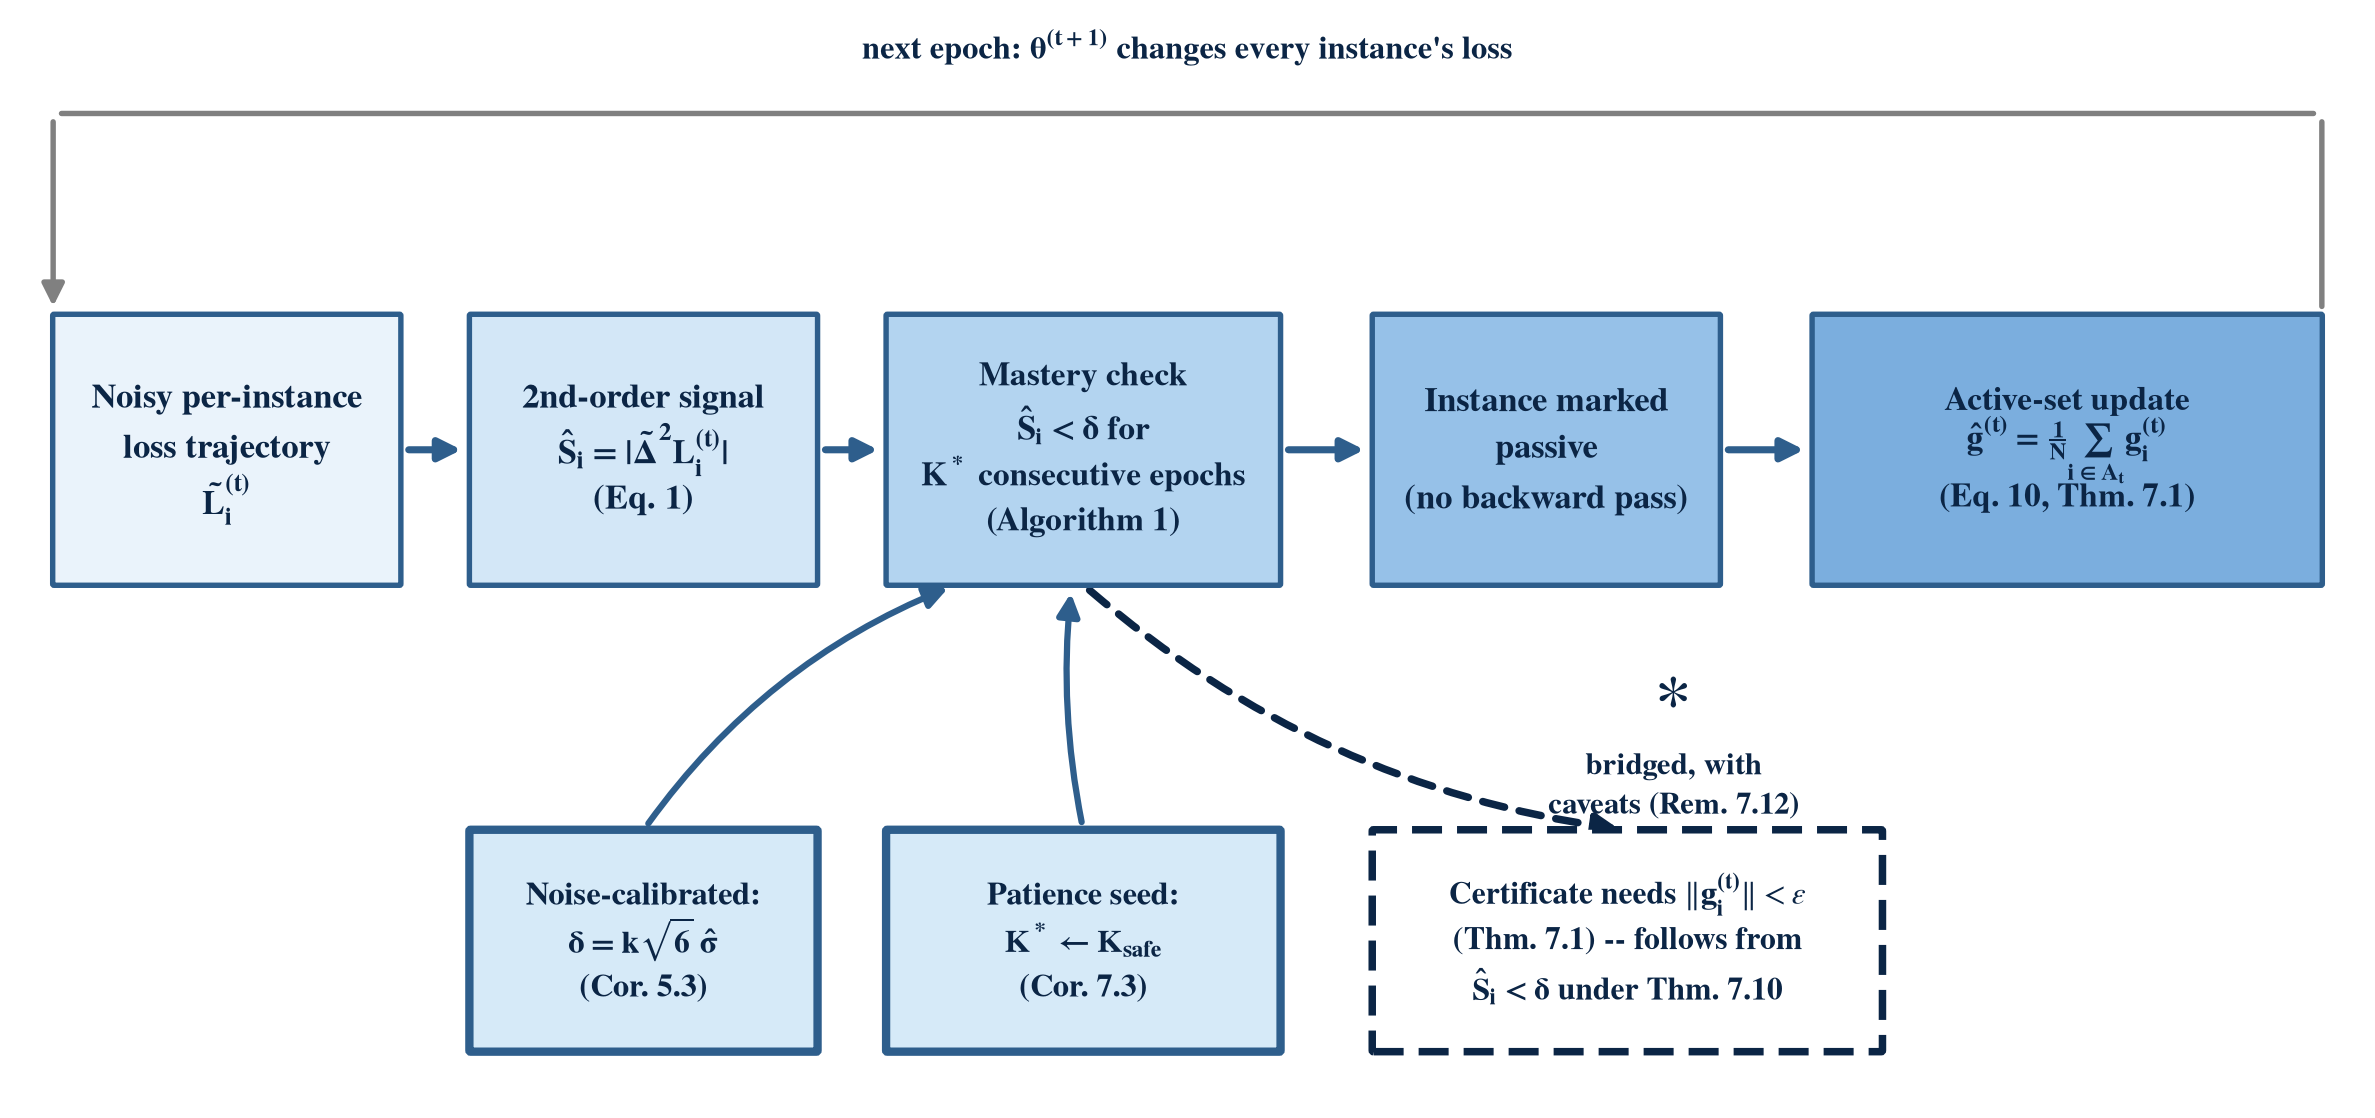
\includegraphics[width=0.92\textwidth]{figures/fig0_overview.png}
\caption{How TG-IES turns a noisy per-instance loss trajectory into a removal decision. The threshold $\delta$ and the patience $K^*$ are each theory-guided (orange), and the mastery check they feed (blue) is now linked to the safety certificate that justifies removal (purple) by \cref{sec:bridge}, under the further idealizations \cref{rem:bridge-scope} states; \cref{sec:ablation} demonstrates directly what goes wrong when those idealizations do not hold closely enough.}
\label{fig:overview}
\end{figure*}

\Cref{fig:overview} summarizes this pipeline; the rest of the paper derives each labeled piece and, in \cref{sec:ablation}, shows what happens when the two theory-guided calibration paths are decoupled from each other.

\section{Related Work}
\label{sec:related}

\textbf{Why training-time compute matters.} The efficiency question this paper's empirical results are ultimately in service of is not academic: training compute for state-of-the-art models has grown roughly $10\times$ every year since 2012 and continues to grow \citep{sevilla2022compute}, with a directly proportional energy and carbon cost \citep{patterson2022carbon}. \citet{bartoldson2023computeefficient}'s survey of algorithmic (rather than hardware) efficiency gains frames exactly the category of method this paper contributes to: a technique that reduces the number of forward/backward passes a fixed training recipe performs, orthogonal to and stackable with hardware- or precision-level efficiency gains. \Cref{sec:flops}'s FLOP-normalized accounting of TG-IES's savings is this paper's own direct, measured contribution to that question, rather than an assumed one.

\textbf{Static data pruning and difficulty scoring.} \citet{toneva2019empirical} track how often an example is learned then forgotten across epochs and show unforgettable examples can be removed with little accuracy loss. \citet{paul2021deep} score examples early in training with the gradient-norm-based EL2N score and prune a static subset before the rest of training. \citet{swayamdipta2020dataset} map examples along confidence and variability axes computed from training dynamics (``dataset cartography'') to separate easy, hard, and ambiguous examples. \citet{coleman2020selection} select a subset using scores from a small, cheap proxy model rather than the target model itself, trading a second training run for a cheaper one. Three more recent entries in this line give the static-pruning side of the field its own theoretical grounding, the same kind of move this paper makes for IES's criterion specifically: \citet{sorscher2022beyond} show, both empirically and via a statistical-mechanics analysis of a toy model, that a good pruning metric can convert the usual power-law scaling of test error with dataset size into exponential scaling, giving a principled account of \emph{why} pruning can beat training on everything; \citet{zheng2023coverage} (CCS) show that pruning to the highest-difficulty examples alone hurts distributional coverage at high pruning rates and instead balance importance against coverage explicitly; \citet{maharana2024d2} (D2 Pruning) use a message-passing formulation over a similarity graph to balance the same difficulty/diversity trade-off. All of these methods commit to a fixed subset before or shortly after training starts; IES and TG-IES instead make a per-instance, per-epoch decision using the current trajectory.

\textbf{Dynamic and online example selection.} \citet{loshchilov2015online} rank minibatches online by loss to bias sampling toward harder examples. \citet{katharopoulos2018not} use a similar importance-sampling argument to reduce gradient variance rather than compute, building on the biased-sampling convergence analysis of \citet{needell2014stochastic}. \citet{jiang2019accelerating} (Selective-Backprop) skip backpropagation, not just sampling, for examples with low relative loss, using a probabilistic accept/reject rule; the qualitative goal (skip backward passes on examples that no longer teach the model much) is close to IES's, but the two are formalized on different arguments (a probabilistic threshold on the loss distribution versus a finite-difference criterion on the loss trajectory) with no theoretical treatment offered on either side. \citet{mindermann2022prioritized} (RHO-LOSS) select points that are simultaneously learnable, worth learning, and not yet learnt using a holdout-model loss criterion; \citet{bankes2024reducr} (REDUCR) extend this line with class-priority reweighting for robustness to class imbalance and distributional shift, a direction orthogonal to the calibration question this paper asks. \citet{qin2024infobatch} (InfoBatch) prune examples below the epoch-mean loss with probability $r$ and rescale the gradient of kept low-score examples by $1/(1-r)$ so that dynamic pruning does not bias the expected gradient, annealing back to the full dataset for the final epochs; unlike IES/TG-IES, InfoBatch skips both the forward and backward pass on a pruned example, at the cost of not re-examining it that epoch at all. \citet{qin2026alignprune} (AlignPrune) replace loss-magnitude ranking with a Dynamic Alignment Score (the correlation between an example's loss trajectory and a reference trajectory over a sliding window) to make pruning robust to label noise, a different objective (noisy-label robustness) than the mastery-based removal IES/TG-IES and InfoBatch target; \citet{nagaraj2025coresets} (Coresets from Trajectories) use a related loss-trajectory-correlation signal, but for one-shot coreset selection against a held-out reference set rather than an online per-epoch removal decision, and give convergence guarantees for the resulting subset -- the closest published criterion to IES/TG-IES's own loss-trajectory signal, differing in using a \emph{held-out reference} correlation rather than a \emph{self-referential} finite difference, and in selecting once rather than deciding, and potentially reversing, every epoch. \citet{zhou2026bls} (BLS) observe that an exponential moving average of loss values is a first-order low-pass filter and use it as a cheap, batch-loss-only proxy for per-sample importance, a signal-processing alternative to TG-IES's noise-calibrated $\delta$ for the same denoising problem. Concurrent with this work, \citet{jin2026orderdp} (OrderDP) also put a formal guarantee under a \emph{dynamic} pruning criterion, but via a different mechanism entirely: an unbiased ranking surrogate with a lossless-convergence proof, rather than the per-instance, per-decision stability certificate \cref{sec:level4} derives here; the two results are best read as two different answers to the same open question (does a dynamic-pruning heuristic admit a real guarantee?) rather than as competitors on the same construction. \citet{zhu2026dppo} address an analogous unbiased-pruning problem for group-based RL policy optimization (GRPO rollout pruning for LLM reasoning); we note it here for completeness, but its setting (sequence-level pruning of policy rollouts) is different enough from per-instance supervised classification that we do not attempt a direct empirical comparison. The same underlying question -- what to spend a gradient update on -- is also being asked one level up, over entire pretraining-data domains rather than individual instances, in large language model pretraining \citep{xie2023doremi}; we mention this only as a pointer to a parallel literature in a different modality and at a coarser granularity, not a method this paper compares against. \Cref{sec:setup,sec:results} compare TG-IES against InfoBatch, BLS, and AlignPrune directly; none of the methods above, including TG-IES's direct predecessor IES, provide a closed-form, theory-guided removal criterion derived from a stability guarantee for the individual per-instance, per-epoch decision IES-family methods make, which is the gap TG-IES targets.

\textbf{Curriculum learning.} \citet{bengio2009curriculum} order examples from easy to hard over the course of training; \citet{soviany2022curriculum} survey the considerable body of work this seeded since. This is complementary to IES/TG-IES: curriculum learning changes when an example enters training, while IES/TG-IES changes when an example leaves it.

\textbf{Direct predecessor.} \citet{yuan2025instance} is the paper this work is theoretically grounding; \cref{sec:intro} details the five gaps we close. Our empirical baselines and architectures follow \citet{he2016deep} (ResNet), \citet{simonyan2015very} (VGG), \citet{krizhevsky2009learning} (CIFAR-10/100), and \citet{dosovitskiy2021image} (Vision Transformer, \cref{sec:vit}).

\section{Preliminaries and Notation}
\label{sec:prelim}

Let $D = \{(x_i,y_i)\}_{i=1}^N$ be the training set and $\theta^{(t)} \in \R^d$ the parameters at epoch $t$. The per-instance loss is $L_i(\theta) = \ell(f_\theta(x_i),y_i)$, with $L_i^{(t)} := L_i(\theta^{(t)})$, and the training objective is $L(\theta) = \frac1N\sum_i L_i(\theta)$. Write $g_i^{(t)} := \nabla_\theta L_i(\theta^{(t)})$ and $g^{(t)} := \nabla_\theta L(\theta^{(t)}) = \frac1N\sum_i g_i^{(t)}$; write $H_i(\theta) := \nabla_\theta^2 L_i(\theta)$. The \emph{observed} (noisy) per-instance loss is $\tilde L_i^{(t)} := L_i^{(t)} + \xi_{i,t}$, a noise model formalized in \cref{ass:noise}. Finite differences are $\Delta^0 L_i^{(t)} = L_i^{(t)}$ and $\Delta^N L_i^{(t)} = \Delta^{N-1}L_i^{(t)} - \Delta^{N-1}L_i^{(t-1)}$. Empirical moments $\mathbb E[\cdot]$, $\Var(\cdot)$, $\CV(\cdot) := \sqrt{\Var(\cdot)}/\mathbb E[\cdot]$ over instances are with respect to $I \sim \mathrm{Unif}\{1,\dots,N\}$. Gradient descent follows $\theta^{(t+1)} = \theta^{(t)} - \eta g^{(t)}$.

All results below hold under one or more of the following explicit idealizations, stated once here so each theorem can cite exactly which ones it needs.

\begin{assumption}[$\beta$-smoothness]
\label{ass:smooth}
$L$ is $\beta$-smooth: $\|\nabla_\theta L(\theta) - \nabla_\theta L(\theta')\| \le \beta\|\theta-\theta'\|$ for all $\theta,\theta'$.
\end{assumption}

\begin{remark}[Why this assumption, and where it is used]
\label{rem:smooth-why}
Intuitively, $\beta$-smoothness caps how fast the gradient can change as the parameters move; it is the standard lever for turning a bound on a single parameter step into a bound that holds over many steps, by controlling how much each step's error can compound into the next. \Cref{app:multistep} now uses it directly, for exactly the purpose anticipated here: a first attempt at extending \cref{thm:safe}'s single-step certificate into a multi-step bound over an entire training run. That attempt succeeds only partially -- it yields a genuine but exponentially-loose bound, not a practically useful one over hundreds of epochs -- and \cref{app:multistep} is explicit about what a tighter argument would still need.
\end{remark}

\begin{assumption}[Local geometric trajectory]
\label{ass:geometric}
Near an optimum $\theta^*$, the per-instance excess loss follows $L_i^{(t)} - L^* = c_i r_i^t$, $c_i>0$, $r_i \in (0,1)$, over the analysis window.
\end{assumption}

\begin{remark}
\label{rem:geometric-scope}
\Cref{ass:geometric} is a local, near-convergence approximation, not a global description of training. Loss trajectories in practice are non-monotonic and noisy, and $r_i$ varies over time; \cref{sec:level1,sec:level2} are exact conditional on this model, and their practical relevance rests on geometric decay being a reasonable local approximation in the late-training regime IES targets.
\end{remark}

\begin{assumption}[Noise: time-independence, finite variance]
\label{ass:noise}
$\tilde L_i^{(t)} = L_i^{(t)} + \xi_{i,t}$ where, conditional on $\theta^{(t)}$, $\xi_{i,t}$ is mean-zero and independent across $t$ for fixed $i$, with $\Var(\xi_{i,t}) = \sigma^2 < \infty$.
\end{assumption}

\begin{assumption}[Sub-Gaussian noise]
\label{ass:subgaussian}
In addition to \cref{ass:noise}, each $\xi_{i,t}$ is $\sigma^2$-sub-Gaussian conditional on $\theta^{(t)}$.
\end{assumption}

\begin{remark}
\label{rem:noise-realism}
\Cref{ass:noise} is an idealization: SGD revisits the same or overlapping minibatches, which correlates noise across nearby $t$. \Cref{ass:subgaussian} may also be violated, since gradient noise in deep learning can be heavy-tailed. Under correlated or heavy-tailed noise, the variance formula in \cref{thm:bv} becomes a lower bound rather than an exact value, and the tail bound in \cref{cor:threshold} may be optimistic.
\end{remark}

\begin{assumption}[Small rate dispersion]
\label{ass:dispersion}
There exist $\bar r \in (0,1)$ and $\delta_r \in (0,1)$ such that $r_i \in [\bar r - \delta_r, \bar r + \delta_r]$ for all $i$, with $\delta_r$ small enough for the first-order expansions in \cref{prop:cv} to hold.
\end{assumption}

\begin{remark}[Why this assumption]
\label{rem:dispersion-why}
$r_i$ is how fast instance $i$'s excess loss decays each epoch (\cref{ass:geometric}); this says different instances' decay rates don't spread too far from a common rate $\bar r$. It is exactly what lets \cref{prop:cv} treat $\CV(X(2))$ as a small perturbation of $\CV(X(1))$ around $\bar r$, via a first-order Taylor argument, one that is only valid when the spread $\delta_r$ it is expanding in is genuinely small. \Cref{app:counterexample} shows explicitly what breaks when it is not: two instances with very different rates can make CV move in the \emph{wrong} direction as $N$ increases, so this is a load-bearing restriction on the training regime, not a technical nicety.
\end{remark}

\begin{assumption}[Uniform bounds on $c_i$]
\label{ass:cbounds}
There exist $0 < c_{\min} \le c_{\max} < \infty$ with $c_i \in [c_{\min},c_{\max}]$ for all $i$.
\end{assumption}

\begin{remark}[Why this assumption]
\label{rem:cbounds-why}
$c_i$ is instance $i$'s excess-loss amplitude in \cref{ass:geometric}: how far above the optimum it starts, before geometric decay kicks in. Bounding it away from both $0$ and $\infty$ does two things: it keeps $\CV(\cdot)=\sqrt{\Var(\cdot)}/\mathbb E[\cdot]$ well-defined (a mean that can approach $0$ makes CV blow up), and it keeps the perturbation constant in \cref{prop:cv} finite and uniform across instances, rather than dominated by one pathologically easy or hard example.
\end{remark}

\begin{assumption}[Bounded third derivatives]
\label{ass:thirdderiv}
There exists $M_3<\infty$ and a neighborhood $U$ of the GD trajectory such that for all $i$, all $\theta\in U$, and unit vectors $u,v,w$: $|\nabla^3 L_i(\theta)[u,v,w]| \le M_3$.
\end{assumption}

\begin{remark}[Why this assumption]
\label{rem:thirdderiv-why}
This bounds how quickly the loss's own curvature can change. It is what keeps the leftover remainder in \cref{thm:curvature}'s third-order Taylor expansion (\cref{app:proofs}) genuinely smaller than the $O(\eta^2)$ curvature term the expansion isolates; without a cap on the third derivative, ``the curvature term is $O(\eta^2)$ and the drift term is $O(\eta)$'' would not be a controlled statement, since an uncontrolled remainder could be larger than either.
\end{remark}

\begin{assumption}[Bounded gradient envelope]
\label{ass:envelope}
On a window $t\in[T-K,T]$, $G := \sup_{t\in[T-K,T]}\|g^{(t)}\| < \infty$.
\end{assumption}

\begin{remark}[This assumption is currently unused]
\label{rem:envelope-why}
Unlike every other assumption in this section, no theorem, corollary, or proof in this paper invokes $G$ under its current proofs. We keep it stated, rather than delete it quietly, because it is a natural quantity for the same future-work extension \cref{rem:smooth-why} names ($\beta$-smoothness plus a bounded gradient envelope is the standard pair needed for a contraction argument bounding trajectory divergence over many steps, \cref{rem:shared-traj}); as things stand in this version, though, it does no formal work, and we say so rather than let a reader hunt for where it is used.
\end{remark}

\section{Level 1: Scale Cancellation Near Convergence}
\label{sec:level1}

\begin{lemma}[Finite differences of geometric sequences]
\label{lem:geomdiff}
Under \cref{ass:geometric}, $\Delta^N(L_i^{(t)}-L^*) = c_i\, r_i^{t-N}(r_i-1)^N$.
\end{lemma}
\begin{proof}
Induction on $N$; see \cref{app:proofs}.
\end{proof}

\begin{theorem}[Exact ratio cancellation]
\label{thm:ratio}
Under \cref{ass:geometric}, for any $N\ge1$ and instance $i$ with $\Delta^{N-1}(L_i^{(t)}-L^*)\ne0$,
\begin{equation}
\label{eq:ratio}
\frac{\Delta^N(L_i^{(t)}-L^*)}{\Delta^{N-1}(L_i^{(t)}-L^*)} = \frac{r_i-1}{r_i}.
\end{equation}
The ratio depends only on $r_i$, not $c_i$; the denominator is nonzero for all finite $t$ under \cref{ass:geometric}.
\end{theorem}
\begin{proof}
Immediate from \cref{lem:geomdiff}: $c_i$ and the shared power of $r_i$ cancel. Full derivation in \cref{app:proofs}.
\end{proof}

\Cref{thm:ratio} is the theorem-level content behind IES's informal ``scale invariance'' claim: it is a ratio identity that eliminates the instance-specific amplitude $c_i$, not a claim that $\Delta^2 L_i$ itself is scale-free.

\begin{proposition}[CV closeness under small rate dispersion]
\label{prop:cv}
Under \cref{ass:geometric,ass:dispersion,ass:cbounds}, let $X_i(N) := |c_i r_i^{t-N}(1-r_i)^N|$ for $N\in\{1,2\}$ at fixed $t$. There is a finite constant $C(t,\bar r,c_{\min},c_{\max})$ such that, for all sufficiently small $\delta_r$,
\begin{equation}
\big|\CV(X(2)) - \CV(X(1))\big| \le C(t,\bar r,c_{\min},c_{\max})\cdot\delta_r.
\end{equation}
\end{proposition}
\begin{proof}
Perturbation/Lipschitz argument around $\bar r$; full proof and explicit constant in \cref{app:proofs,app:constants}.
\end{proof}

\Cref{prop:cv} shows $\CV(X(2))$ and $\CV(X(1))$ are close, within $O(\delta_r)$, when rate dispersion is small; it does not assert $N=2$ globally reduces dispersion. \Cref{app:counterexample} gives an explicit counterexample showing global CV monotonicity can fail under large rate dispersion, confirming \cref{ass:dispersion} is load-bearing, not a technicality.

\section{Level 2: Noise-Optimality of $N=2$}
\label{sec:level2}

\begin{theorem}[Exact bias--variance decomposition]
\label{thm:bv}
Under \cref{ass:geometric,ass:noise},
\begin{equation}
\label{eq:bv}
\mathbb E\big[(\Delta^N \tilde L_i^{(t)})^2\big] = c_i^2 r_i^{2(t-N)}(r_i-1)^{2N} + \binom{2N}{N}\sigma^2.
\end{equation}
\end{theorem}
\begin{proof}
Linearity of the finite-difference operator splits $\Delta^N\tilde L_i^{(t)}$ into a deterministic part (\cref{lem:geomdiff}) plus $\Delta^N\xi_{i,t}$; the cross term vanishes by \cref{ass:noise}, and the noise variance follows from the Vandermonde identity $\sum_k \binom{N}{k}^2 = \binom{2N}{N}$. Full proof in \cref{app:proofs}.
\end{proof}

Variance scales combinatorially in the order $N$ ($\binom{2}{1}=2$, $\binom{4}{2}=6$, $\binom{6}{3}=20$), which is the quantitative reason high-order differencing is costly and a low order is preferable.

\begin{proposition}[$N=2$ is MSE-optimal for $r_i>\tfrac12$]
\label{prop:mse}
Under \cref{ass:geometric,ass:noise}, define $\mathrm{MSE}(N,t) := c_i^2 r_i^{2(t-N)}(r_i-1)^{2N} + \binom{2N}{N}\sigma^2$ and $\alpha_i := (1-r_i)^2/r_i^2$. Then
\begin{align}
\mathrm{MSE}(2,t)\!\le\!\mathrm{MSE}(1,t) &\iff c_i^2 r_i^{2t}\alpha_i(1-\alpha_i) \ge 4\sigma^2, \label{eq:mse12}\\
\mathrm{MSE}(2,t)\!\le\!\mathrm{MSE}(3,t) &\iff c_i^2 r_i^{2t}\alpha_i^2(1-\alpha_i) \le 14\sigma^2. \label{eq:mse23}
\end{align}
If $r_i>\tfrac12$ (equivalently $\alpha_i<1$), $N=2$ minimizes MSE over $\{1,2,3\}$ whenever
\begin{equation}
\label{eq:band}
\frac{4\sigma^2}{\alpha_i(1-\alpha_i)} \;\le\; c_i^2 r_i^{2t} \;\le\; \frac{14\sigma^2}{\alpha_i^2(1-\alpha_i)},
\end{equation}
and this band is non-empty for every $\alpha_i<1$ (i.e., $4\alpha_i \le 14$ always holds there).
\end{proposition}
\begin{proof}
\Cref{app:proofs}.
\end{proof}

This is the first explicit, checkable SNR regime in which $N=2$ is MSE-optimal among low orders; it is conditional on \cref{ass:geometric,ass:noise} and restricted to $r_i>\tfrac12$, where $(1-\alpha_i)$ is guaranteed positive.

\textbf{Direct empirical test.} \Cref{prop:mse}'s claim is about the SNR regime \cref{eq:band} describes, not about every instance at every epoch; a naive population-average test that ignores this (computing empirical MSE$(N)$ pooling all instances across an entire late-training window, dominated by already-converged instances where the noise floor's own $\binom{2N}{N}$ growth makes $N=1$ win trivially) finds $N=1$ beats $N=2$ -- the opposite of \cref{prop:mse}'s claim, and true even restricted to a coarse "still-decaying" (loss-magnitude) proxy for the band. The fair test evaluates each instance exactly at the moment its own $|\Delta^2 L_i^{(t)}|$ first drops below the calibrated $\delta{=}0.01597$ (the actual operating point \cref{alg:tgies}'s mastery check uses, from the exponential-schedule diagnostic run of \cref{sec:lrmechanism}), not a proxy for it: there, pooling over the $46{,}779$ instances with enough training history, $N{=}2$ gives the lowest MSE ($7.5\times10^{-5}$) by roughly two orders of magnitude over $N{=}1$ ($2.3\times10^{-2}$) and three over $N{=}3$ ($0.58$), confirming \cref{prop:mse}'s claim exactly where it is meant to apply. We report both tests rather than only the confirming one, since the contrast is itself informative: \cref{prop:mse}'s SNR band is a real, non-vacuous restriction, not a technical qualifier that happens to hold everywhere.

\begin{figure}[t]
\centering
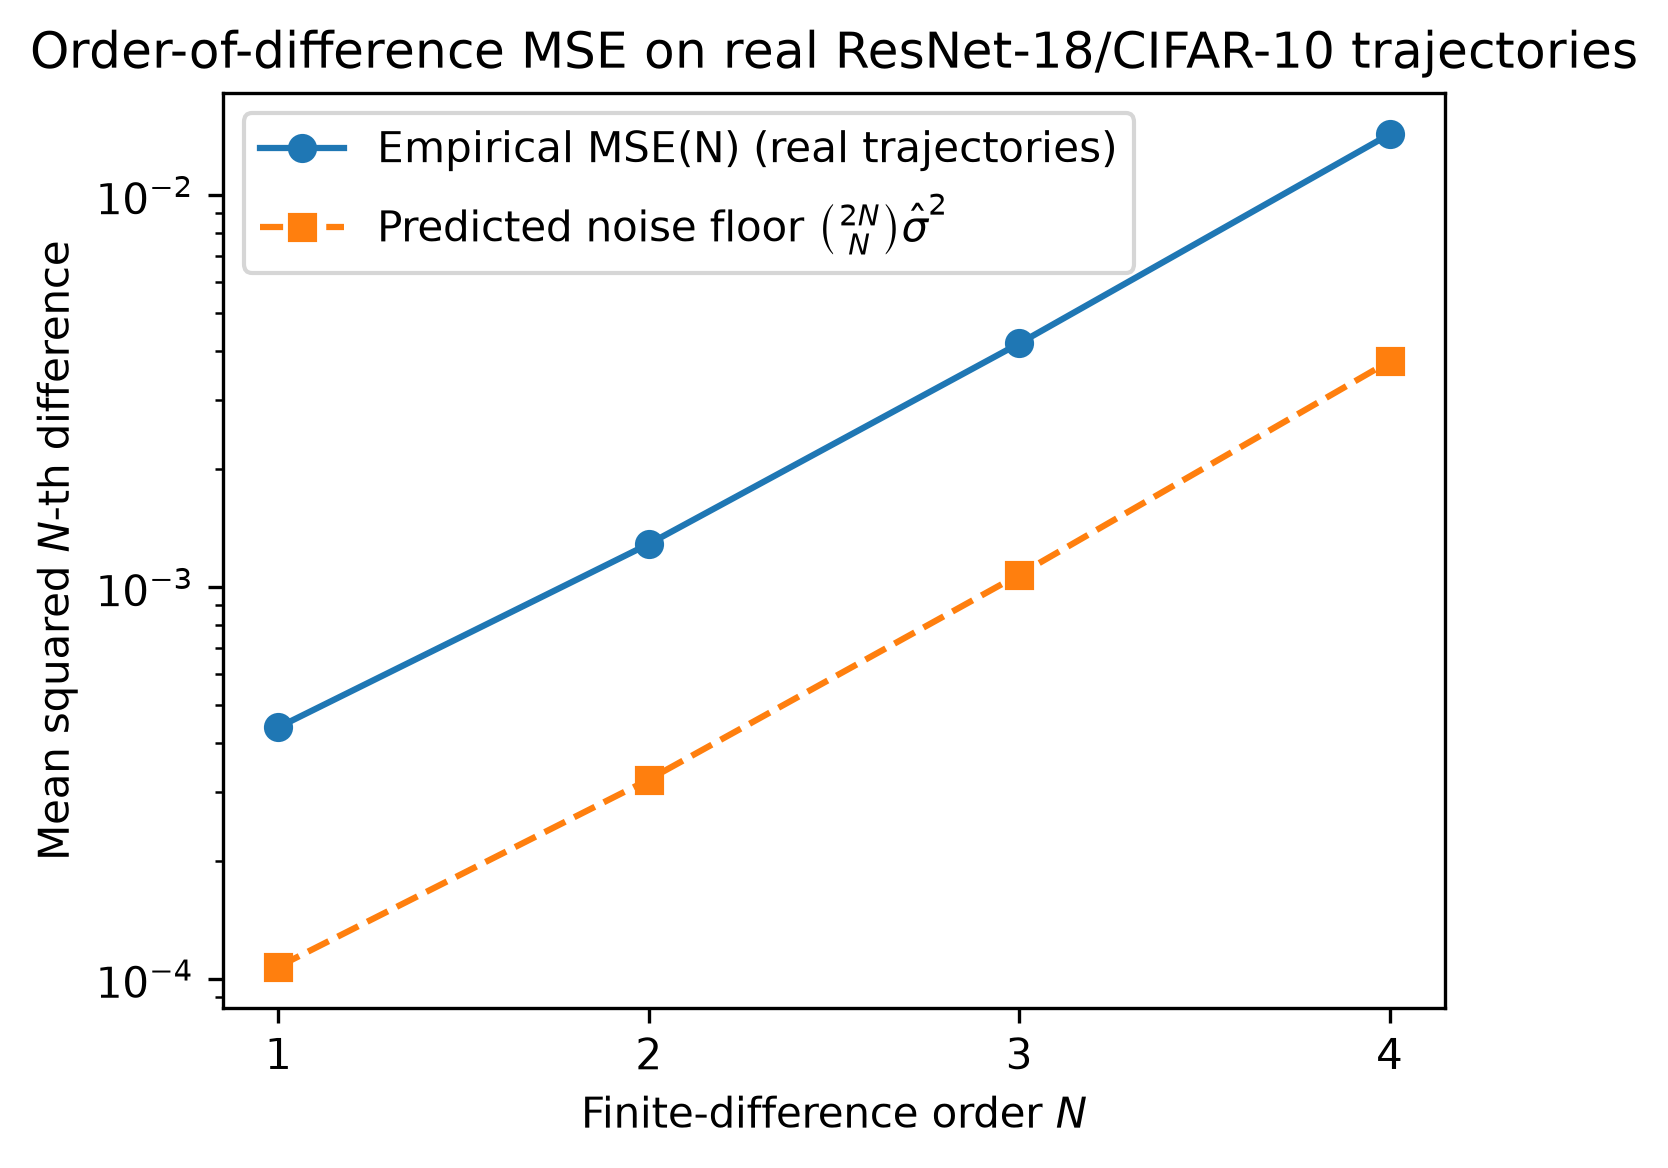
\includegraphics[width=\columnwidth]{figures/fig_order_of_difference.png}
\caption{Empirical MSE$(N)$ vs.\ predicted noise floor $\binom{2N}{N}\hat\sigma^2$, naive population-average test (all instances, epochs 101--200, ResNet-18/CIFAR-10/exponential seed 0). This pooled test does not isolate \cref{prop:mse}'s SNR band and finds $N{=}1$ lowest; the band-restricted test at each instance's own calibration crossing (reported in text) finds $N{=}2$ lowest, as \cref{prop:mse} predicts.}
\label{fig:orderdiff}
\end{figure}

\textbf{Training-phase dependence of $r_i$.} \Cref{ass:geometric} models each instance's loss as decaying at a fixed rate $r_i$ throughout training; we check how well this holds across training phases by estimating $\hat r_i(t) := \Delta^1 L_i^{(t+1)}/\Delta^1 L_i^{(t)}$ (\cref{thm:ratio}'s own ratio statistic) per epoch-quartile, pooling over all still-decreasing instance-epoch pairs in each quartile (ResNet-18/CIFAR-10, exponential schedule, full 200-epoch trajectory). The estimated rate is not constant across training: mean $\hat r$ rises from $0.53$ (epochs 1--50) to $0.54$ (51--100) to $0.74$ (101--150) to $0.76$ (151--199), while its coefficient of variation falls from $1.05$ to $0.75$ over the same span -- instances decay faster and more heterogeneously early in training, then slow down and homogenize later, consistent with \cref{ass:geometric} being a better approximation in the second half of training than the first. This is additional evidence, alongside \cref{sec:practical}'s empirical finding that recalibrating once at epoch 30 (rather than immediately or repeatedly) works best, that the theory's late-training regime and the algorithm's actual operating regime already coincide by design, though we did not derive the epoch-30 choice from this quartile analysis and do not claim a precise match.

\begin{figure}[t]
\centering
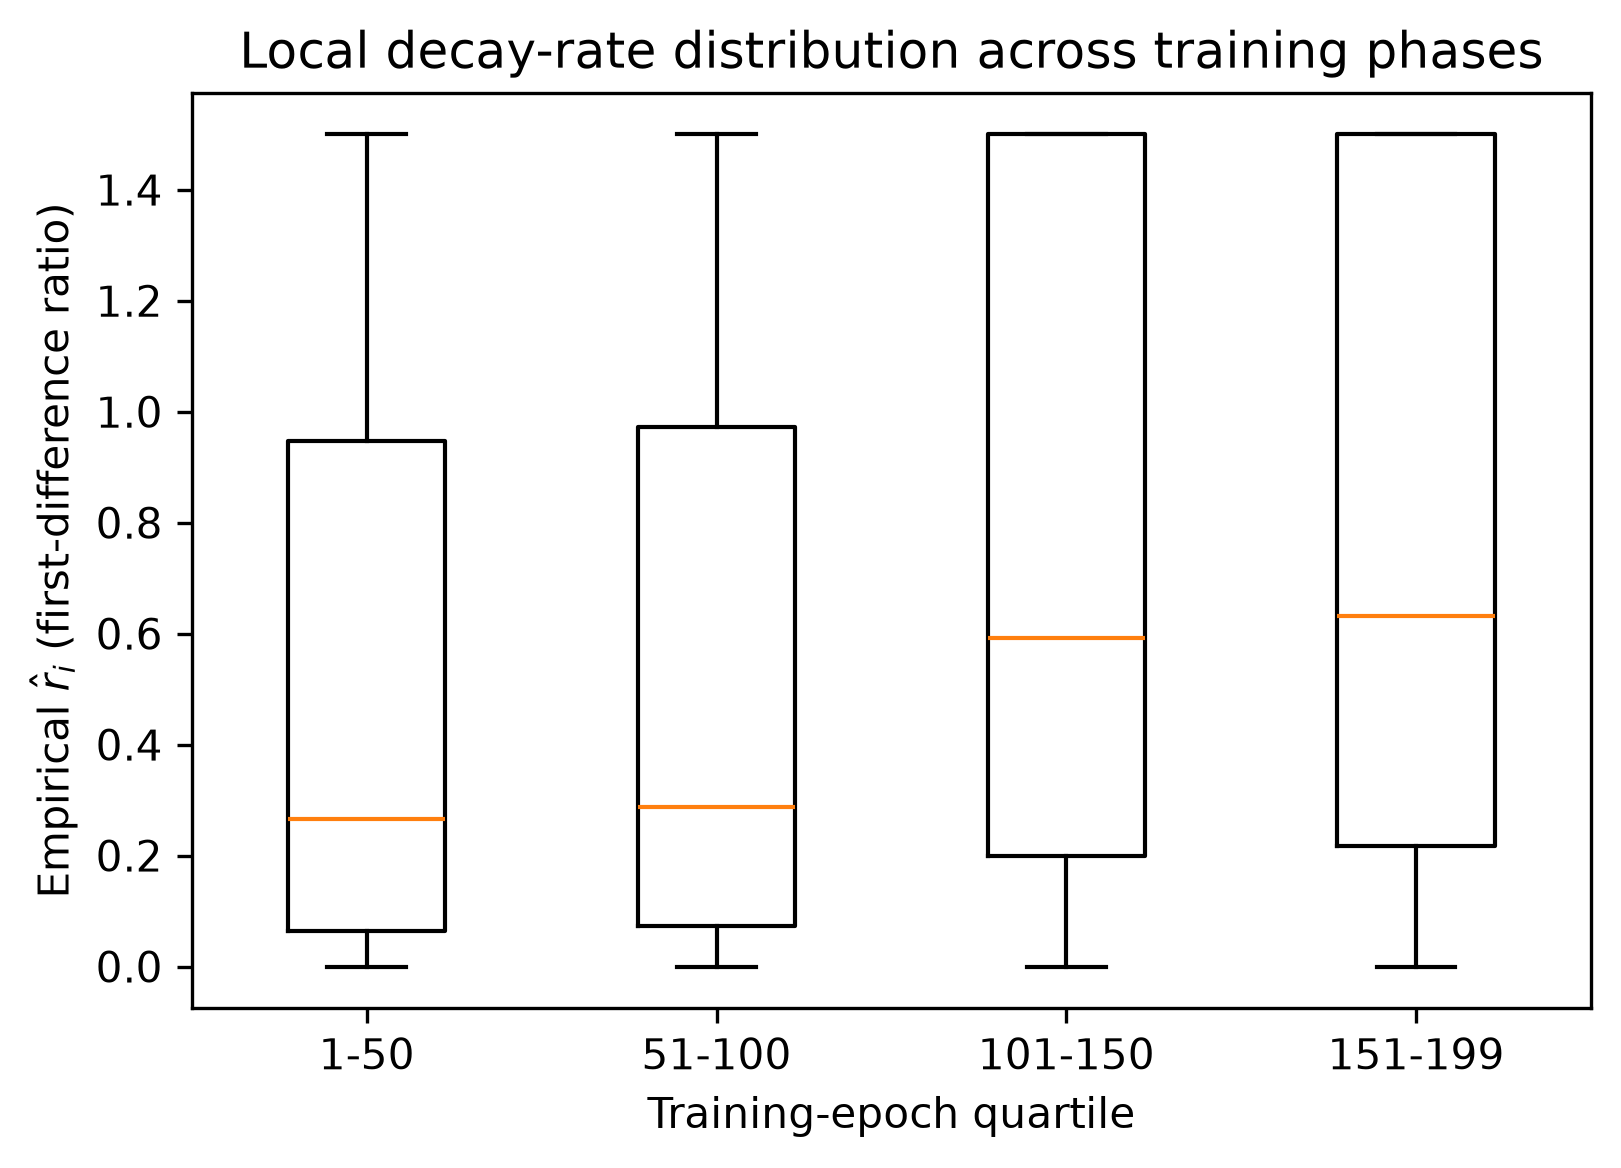
\includegraphics[width=\columnwidth]{figures/fig_phase_quartile_r.png}
\caption{Empirical $\hat r_i$ (first-difference ratio, \cref{thm:ratio}) pooled per training-epoch quartile, ResNet-18/CIFAR-10/exponential seed 0. Boxes show the pooled distribution (outliers omitted); the rate rises and its spread narrows in the second half of training.}
\label{fig:phasequartile}
\end{figure}

\begin{corollary}[Threshold calibration]
\label{cor:threshold}
Under \cref{ass:noise,ass:subgaussian}, $\Delta^2\xi_{i,t}$ is mean-zero with variance $6\sigma^2$. Setting $\delta = k\sqrt6\,\sigma$: if $\Delta^2\xi_{i,t}$ is approximately Gaussian, $\Pr(|\Delta^2\xi_{i,t}|>\delta)\approx 2(1-\Phi(k))$; in general, under \cref{ass:subgaussian}, $\Pr(|\Delta^2\xi_{i,t}|>\delta) \le 2\exp(-k^2/2)$.
\end{corollary}
\begin{proof}
$\Delta^2\xi_{i,t} = \xi_{i,t}-2\xi_{i,t-1}+\xi_{i,t-2}$ has squared coefficients $1^2+(-2)^2+1^2=6$, so it is $6\sigma^2$-sub-Gaussian; apply the standard sub-Gaussian tail bound and Gaussian approximation. Full proof in \cref{app:proofs}.
\end{proof}

\Cref{cor:threshold} turns $\delta$ from a hand-tuned constant into a function of an estimated noise scale $\hat\sigma$ and a target tail probability $k$, the calibration TG-IES uses online (\cref{sec:level4}).

\section{Level 3: A Corrected Curvature Reading}
\label{sec:level3}

\begin{theorem}[Backward second-difference decomposition]
\label{thm:curvature}
Under \cref{ass:thirdderiv}, along full-batch GD,
\begin{multline}
\label{eq:curvature}
\Delta^2 L_i^{(t)} = \eta\Big(\langle g_i^{(t-2)},g^{(t-2)}\rangle - \langle g_i^{(t-1)},g^{(t-1)}\rangle\Big) \\
{}+ \frac{\eta^2}{2}g^{(t-1)\top}H_i(\theta^{(t-1)})g^{(t-1)} \\
{}- \frac{\eta^2}{2}g^{(t-2)\top}H_i(\theta^{(t-2)})g^{(t-2)} + R_{i,t},
\end{multline}
with remainder bounded as
\begin{equation}
\label{eq:remainder-bound}
|R_{i,t}| \le \tfrac{M_3}{6}\eta^3\big(\|g^{(t-1)}\|^3+\|g^{(t-2)}\|^3\big).
\end{equation}
\end{theorem}
\begin{proof}
Third-order Taylor expansion of $L_i$ at $s=t-1$ and $s=t-2$ along $\Delta\theta^{(s)}=-\eta g^{(s)}$, then form the backward second difference; the $O(\eta)$ and $O(\eta^2)$ terms separate cleanly and the remainders combine by the triangle inequality. Full proof in \cref{app:proofs}.
\end{proof}

\Cref{thm:curvature} shows $\Delta^2 L_i$ is \emph{not} a pure curvature proxy: it contains an $O(\eta)$ gradient-drift term $\eta\,\Delta(\langle g_i,g\rangle)$ alongside the $O(\eta^2)$ curvature term $\frac{\eta^2}2\Delta(g^\top H_i g)$, an asymptotic ($\eta\to0$) ordering in which the drift term is the leading one; only near convergence, where gradients are small, do both vanish together, consistent with the geometric model of \cref{ass:geometric}. Omitting the drift term, as a purely-curvature reading would, misdescribes what the mastery signal measures. Whether the drift term also dominates \emph{in absolute magnitude} at this paper's actual step sizes, rather than only in the $\eta\to0$ asymptotic ordering, is an empirical question we instrument and check directly in \cref{sec:lrmechanism}; the answer there is more qualified than a leading-order reading of this decomposition alone would suggest.

\begin{remark}[Scope: full-batch vs.\ active-set gradient]
\label{rem:activeset}
\Cref{thm:curvature} is stated for the full-batch update. Algorithm~\ref{alg:tgies} uses the scaled active-set gradient $\hat g^{(t)} = \frac1N\sum_{i\in A_t}g_i^{(t)}$ (\cref{eq:activegrad}) in its place; \cref{eq:curvature} extends unchanged with every $g^{(s)}$ replaced by $\hat g^{(s)}$, and the remainder bound is no weaker since $\|\hat g^{(s)}\| \le \|g^{(s)}\|$. The curvature reading therefore applies to the algorithm as implemented, not only to idealized full-batch GD.
\end{remark}

\section{Removal Perturbation Bounds and a Certified Exclusion Horizon}
\label{sec:level4}

To keep the update on the same $1/N$ scale as full-batch GD while skipping passive instances, TG-IES uses the scaled active-set gradient
\begin{equation}
\label{eq:activegrad}
\hat g^{(t)} = \frac1N \sum_{i\in A_t} g_i^{(t)},
\end{equation}
where $A_t$ is the active set at epoch $t$. This differs from the shipped IES normalization, which divides by $|A_t|$ (a mean over the active set, not $N$): dividing by the shrinking $|A_t|$ increases the effective step size as instances are excluded, whereas \cref{eq:activegrad} shrinks proportionally to the amount excluded, trading the shipped normalization's implicit speed heuristic for the stability bound below.

\begin{theorem}[Conditional local stability certificate, under a shared-reference trajectory]
\label{thm:safe}
Suppose instance $i$ satisfies $\|g_i^{(t)}\| < \varepsilon$ for all $t\in[T-K,T]$. Consider two runs sharing the same reference trajectory $\{\theta^{(t)}\}_{t=T-K}^T$, both using update \cref{eq:activegrad} evaluated on that trajectory, differing only in whether $i \in A_t$ for $t\in[T-K,T]$. Then
\begin{equation}
\label{eq:safe}
\big\|\theta^{(T)}_{\mathrm{full}} - \theta^{(T)}_{\mathrm{rem}}\big\| \le \frac{K\eta\varepsilon}{N}.
\end{equation}
If additionally the test loss $L_{\mathrm{test}}$ is $\beta_{\mathrm{test}}$-Lipschitz in parameters,
$\big|L_{\mathrm{test}}(\theta^{(T)}_{\mathrm{full}}) - L_{\mathrm{test}}(\theta^{(T)}_{\mathrm{rem}})\big| \le \beta_{\mathrm{test}} K\eta\varepsilon/N$.
\end{theorem}
\begin{proof}
Both updates share every term except $\frac1N g_i^{(t)}$; the per-step deviation is bounded by $\eta\varepsilon/N$, and summing over $K$ steps (triangle inequality) gives \cref{eq:safe}. Full proof in \cref{app:proofs}.
\end{proof}

\begin{remark}[Scope of the idealization: why this is a \emph{conditional, local} certificate, not a training-run guarantee]
\label{rem:shared-traj}
\Cref{thm:safe} compares two hypothetical runs evaluated on the \emph{same} reference trajectory; an actual run's two counterfactual trajectories would diverge from the moment $i$ is removed, since later updates then differ. We are explicit about naming what kind of result this is, since it is easy to read ``certified exclusion horizon'' as more than what is proved: it is a \emph{conditional} certificate (conditional on the shared-reference-trajectory idealization holding) and a \emph{local} one (bounding only the instantaneous, single-window perturbation a removal decision induces, evaluated at one point in training), not a guarantee that Algorithm~\ref{alg:tgies}'s actual, multi-removal training trajectory stays within any bounded distance of the full-data trajectory over the course of training. Concretely: nothing here rules out compounding drift as more instances are removed and the two trajectories accumulate divergence over hundreds of epochs. Bounding that would need a genuinely different result -- a multi-step trajectory-divergence bound under further contraction arguments (e.g., via \cref{ass:smooth}); \cref{app:multistep} reports a first attempt (a correct but exponentially-loose bound, \cref{prop:multistep}), listed as the central open theoretical question in \cref{sec:limitations}, not a closed one. \Cref{sec:kstartraj} instruments the actual, compounding version of this quantity directly and finds it does not blow up over $200$ epochs on the primary cell, empirical evidence against the worst-case failure mode this remains open to, though not a substitute for a proof.
\end{remark}

\begin{corollary}[Certified exclusion horizon]
\label{cor:kstar}
Given a tolerance $\tau>0$ on test-loss deviation, \cref{eq:safe} certifies that \emph{any} exclusion window of length $K$ satisfying
\begin{equation}
\label{eq:kstar}
K \;\le\; K_{\mathrm{safe}} \;:=\; \left\lfloor \frac{N\tau}{\beta_{\mathrm{test}}\,\eta\,\varepsilon} \right\rfloor
\end{equation}
keeps $|L_{\mathrm{test}}(\theta^{(T)}_{\mathrm{full}})-L_{\mathrm{test}}(\theta^{(T)}_{\mathrm{rem}})|\le\tau$. $K_{\mathrm{safe}}$ is the \emph{largest} integer satisfying the tolerance constraint, hence a floor, not a ceiling: rounding up instead would admit a $K$ that violates \cref{eq:safe}.
\end{corollary}
\begin{proof}
$\beta_{\mathrm{test}}K\eta\varepsilon/N \le \tau \iff K \le N\tau/(\beta_{\mathrm{test}}\eta\varepsilon)$; the largest integer $K$ satisfying this is $\lfloor N\tau/(\beta_{\mathrm{test}}\eta\varepsilon)\rfloor$.
\end{proof}

\begin{remark}[$K_{\mathrm{safe}}$ is not Algorithm~\ref{alg:tgies}'s patience]
\label{rem:kmismatch}
$K_{\mathrm{safe}}$ certifies how long an \emph{already-excluded} instance may remain excluded, counted backward from a fixed endpoint $T$ on a shared reference trajectory (\cref{thm:safe}), an upper bound on an exclusion window whose start and end are both given. Algorithm~\ref{alg:tgies}'s patience $K^*$ answers a different question: how many consecutive low-signal epochs must elapse \emph{before} an instance is first marked passive, after which its exclusion is open-ended (it stays passive until it is reactivated, if ever, or until training ends) rather than a fixed $K$-epoch window. No result in this paper shows that seeding the patience counter with $K_{\mathrm{safe}}$ (i.e., setting $K^*\leftarrow K_{\mathrm{safe}}$ as Algorithm~\ref{alg:tgies} does) keeps that open-ended, revocable exclusion inside the budget \cref{cor:kstar} certifies for a closed window of known length. We use $K_{\mathrm{safe}}$ to calibrate $K^*$ as a principled, non-arbitrary quantity to seed patience with, not as a proof that the resulting patience is itself safe; this is a second, distinct gap from \cref{rem:open}, and closing it (relating detection delay to certified exclusion duration under Algorithm~\ref{alg:tgies}'s actual removal dynamics) is left to future work.
\end{remark}

\begin{remark}[An open problem, and where it is now partly closed]
\label{rem:open}
Independently of \cref{rem:kmismatch}, Algorithm~\ref{alg:tgies} removes instance $i$ when the \emph{noisy} signal $\hat S_i = |\tilde L_i^{(t)}-2\tilde L_i^{(t-1)}+\tilde L_i^{(t-2)}|$ stays below $\delta$ for $K^*$ consecutive epochs; \cref{thm:safe} requires $\|g_i^{(t)}\|<\varepsilon$. These two conditions are not linked by any result stated so far. The natural route would use \cref{thm:curvature}: $\hat S_i<\delta$ constrains the drift term $\eta(\langle g_i^{(t-2)},g^{(t-2)}\rangle-\langle g_i^{(t-1)},g^{(t-1)}\rangle)$, and by Cauchy--Schwarz each inner product relates to $\|g_i^{(t)}\|$ if the angle between $g_i^{(t)}$ and $g^{(t)}$ stays bounded away from $90^\circ$. This route does not actually close the gap, though: the drift term is a \emph{difference} of two inner products, so its smallness shows the two are close to each other across consecutive epochs, not that either is small in absolute terms — an instance with a large but stable $\langle g_i^{(t)},g^{(t)}\rangle$ could trigger $\hat S_i<\delta$ indefinitely without $\|g_i^{(t)}\|$ ever shrinking. \Cref{sec:bridge} closes the gap by a different route instead, through the geometric-decay model of \cref{ass:geometric} rather than the curvature decomposition of \cref{thm:curvature}, at the cost of further stated idealizations (\cref{thm:bridge,cor:bridgeprob}); \cref{rem:bridge-scope} states precisely what that route does and does not resolve. Until then, and to the extent those further idealizations do not hold, $\delta$ (\cref{cor:threshold}) and $K^*$ (\cref{cor:kstar}) should still be treated as \emph{independently} calibrated, each with its own theoretical backing but no joint guarantee beyond \cref{sec:bridge}. We surface this rather than paper over it, since \cref{sec:results} shows a failure case plausibly connected to exactly this gap.
\end{remark}

\subsection{Closing the Gap: From Mastery Signal to Gradient Norm}
\label{sec:bridge}

We close \cref{rem:open}'s gap directly: under two further idealizations beyond \cref{ass:geometric}, the noiseless mastery signal $\Delta^2 L_i^{(t)}$ provably bounds $\|g_i^{(t)}\|$, and the observed, noisy $\hat S_i$ bounds it with high probability.

\begin{assumption}[Per-instance smoothness]
\label{ass:smoothi}
Each per-instance loss $L_i$ is $\Lambda_i$-smooth on the same neighborhood $U$ of the late-training trajectory and $\theta^*$ that \cref{ass:geometric} is stated on: $\|\nabla_\theta L_i(\theta)-\nabla_\theta L_i(\theta')\|\le\Lambda_i\|\theta-\theta'\|$ for $\theta,\theta'\in U$.
\end{assumption}

\begin{remark}[Why this assumption]
\label{rem:smoothi-why}
This is the natural per-instance analogue of \cref{ass:smooth}, which is already stated only for the population loss $L=\frac1N\sum_i L_i$; \cref{ass:smooth} follows from \cref{ass:smoothi} with $\beta\le\max_i\Lambda_i$ by the triangle inequality, so this sharpens an idealization already in the paper to hold instance-by-instance rather than introducing an unrelated one. We also read \cref{ass:geometric}'s shared reference value $L^*$ (written with no instance subscript) literally here, as $L_i(\theta^*)=L^*$ at the \emph{same} $\theta^*$ for every $i$: the interpolating-solution regime standard for overparameterized networks late in training, where every instance's loss can reach a common floor at, or near, the same point.
\end{remark}

\begin{lemma}[Smoothness bounds the gradient by suboptimality]
\label{lem:descent}
If $f$ is $\Lambda$-smooth on a neighborhood $U$ and $\theta^*\in U$ satisfies $f(\theta^*)\le f(\theta-\tfrac1\Lambda\nabla f(\theta))$ for all $\theta\in U$ with $\theta-\tfrac1\Lambda\nabla f(\theta)\in U$, then $\|\nabla f(\theta)\|^2 \le 2\Lambda(f(\theta)-f(\theta^*))$ for all such $\theta$.
\end{lemma}
\begin{proof}
\emph{Proof idea:} take one gradient step of size $1/\Lambda$ from $\theta$; $\Lambda$-smoothness bounds how much this single step can decrease $f$, and $\theta^*$ being at least as good as the point reached turns that bound directly into a bound on $\|\nabla f(\theta)\|$.

By the descent lemma (a direct consequence of $\Lambda$-smoothness via Taylor's theorem with remainder; no convexity is needed), $f(\theta-\tfrac1\Lambda\nabla f(\theta)) \le f(\theta) - \tfrac1{2\Lambda}\|\nabla f(\theta)\|^2$. Combined with the hypothesis $f(\theta^*)\le f(\theta-\tfrac1\Lambda\nabla f(\theta))$, this gives $f(\theta^*) \le f(\theta)-\tfrac1{2\Lambda}\|\nabla f(\theta)\|^2$, which rearranges to the claim.
\end{proof}

\begin{remark}[Scope of the minimizer condition]
\label{rem:descent-scope}
The hypothesis on $\theta^*$ holds automatically if $\theta^*$ globally minimizes $f$; we invoke it in the weaker, local form stated, consistent with \cref{ass:geometric} itself being a local, late-training idealization (\cref{rem:geometric-scope}) rather than a global claim about $L_i$'s shape everywhere.
\end{remark}

\begin{theorem}[Mastery bounds the gradient norm]
\label{thm:bridge}
Under \cref{ass:geometric,ass:smoothi}, with \cref{lem:descent}'s hypothesis satisfied for $f=L_i$ at $\theta^*$, for $t$ in the window \cref{ass:geometric} governs,
\begin{equation}
\label{eq:bridge}
\|g_i^{(t)}\| \;\le\; \frac{r_i}{1-r_i}\sqrt{2\Lambda_i\,\Delta^2 L_i^{(t)}}.
\end{equation}
In particular, $\Delta^2 L_i^{(t)} < \delta$ implies $\|g_i^{(t)}\| < \varepsilon_i(\delta) := \frac{r_i}{1-r_i}\sqrt{2\Lambda_i\delta}$.
\end{theorem}
\begin{proof}
\emph{Proof idea:} \cref{lem:descent} bounds $\|g_i^{(t)}\|$ by the noiseless excess loss $L_i^{(t)}-L^*$; \cref{ass:geometric} gives that excess loss in closed form as $c_i r_i^t$; and \cref{lem:geomdiff} gives an exact closed form for $\Delta^2 L_i^{(t)}$ in the same $c_i,r_i$. Combining the two closed forms algebraically eliminates $c_i$ and leaves a bound purely in terms of the observable $\Delta^2 L_i^{(t)}$.

By \cref{lem:descent}, $\|g_i^{(t)}\|^2 \le 2\Lambda_i(L_i^{(t)}-L^*) = 2\Lambda_i c_i r_i^t$ (\cref{ass:geometric}). By \cref{lem:geomdiff} at $N=2$, $\Delta^2 L_i^{(t)} = c_i r_i^{t-2}(1-r_i)^2 \ge 0$, so $c_i r_i^{t-2} = \Delta^2 L_i^{(t)}/(1-r_i)^2$ and $c_i r_i^t = r_i^2 \cdot c_i r_i^{t-2} = \big(r_i/(1-r_i)\big)^2 \Delta^2 L_i^{(t)}$. Substituting gives $\|g_i^{(t)}\|^2 \le 2\Lambda_i\big(r_i/(1-r_i)\big)^2\Delta^2 L_i^{(t)}$, and taking square roots gives \cref{eq:bridge}.
\end{proof}

\begin{corollary}[Probabilistic bridge under observation noise]
\label{cor:bridgeprob}
Under \cref{thm:bridge}'s assumptions plus \cref{ass:subgaussian}, for any $k>0$ and $\delta':=\delta+k\sqrt6\,\sigma$,
\begin{equation}
\Pr\big(\hat S_i<\delta \text{ and } \|g_i^{(t)}\|\ge\varepsilon_i(\delta')\big) \;\le\; 2\exp(-k^2/2).
\end{equation}
\end{corollary}
\begin{proof}
\emph{Proof idea:} the observed $\hat S_i$ and the true $\Delta^2 L_i^{(t)}$ differ only by the noise term $\Delta^2\xi_{i,t}$ (\cref{cor:threshold}); if that noise term is small, $\hat S_i<\delta$ forces $\Delta^2 L_i^{(t)}$ to not exceed $\delta$ by much, and \cref{thm:bridge} then bounds $\|g_i^{(t)}\|$. The only way the conclusion can fail is if the noise term is large, an event \cref{cor:threshold}'s sub-Gaussian tail bound already controls.

$\Delta^2 L_i^{(t)} = \hat S_i \mp \Delta^2\xi_{i,t}$ up to the sign of $\Delta^2\xi_{i,t}$, so $\hat S_i<\delta$ together with $|\Delta^2\xi_{i,t}|\le k\sqrt6\sigma$ implies $\Delta^2 L_i^{(t)} < \delta+k\sqrt6\sigma=\delta'$, hence by \cref{thm:bridge}, $\|g_i^{(t)}\|<\varepsilon_i(\delta')$. So the event in the statement is contained in $\{|\Delta^2\xi_{i,t}|>k\sqrt6\sigma\}$, which \cref{cor:threshold} bounds by $2\exp(-k^2/2)$.
\end{proof}

\begin{remark}[What this does and does not close]
\label{rem:bridge-scope}
\Cref{thm:bridge,cor:bridgeprob} give the link \cref{rem:open} names as missing, but under two further idealizations, not for free, and with two remaining caveats. The idealizations are \cref{ass:smoothi} and reading \cref{ass:geometric}'s $L^*$ as a literal shared value $L_i(\theta^*)$ (\cref{rem:smoothi-why}); \cref{sec:limitations} lists both as open scope questions like every other idealization in this paper. The first caveat: $\varepsilon_i(\delta)\propto r_i/(1-r_i)$ grows without bound as $r_i\to1$, so the bridge is only informative for instances decaying at a genuine rate, not ones whose small $\Delta^2 L_i$ reflects being nearly stationary rather than nearly converged, precisely the regime \cref{rem:geometric-scope} already flags as outside \cref{ass:geometric}'s intended reach. The second: \cref{cor:bridgeprob} bounds a \emph{joint} probability, $\Pr(\hat S_i<\delta\text{ and }\|g_i^{(t)}\|\ge\varepsilon_i(\delta'))$, not the conditional $\Pr(\|g_i^{(t)}\|\ge\varepsilon_i(\delta')\mid \hat S_i<\delta)$: since $\hat S_i$ and $\Delta^2\xi_{i,t}$ share the same noise, conditioning on $\hat S_i<\delta$ shifts the effective distribution of $\Delta^2\xi_{i,t}$, and bounding the resulting conditional tail rigorously would need a prior on $\Delta^2 L_i^{(t)}$ this paper does not assume. We report the joint bound because it is what we can prove without that extra assumption; it is also arguably the more directly useful statement for a safety argument, since it bounds how often ``mastery check passes while the gradient is still large'' happens at all, rather than a probability conditioned on an event built from the same randomness being bounded.
\end{remark}

\textbf{Empirical check.} \Cref{thm:bridge}'s bound needs a per-instance decay rate $r_i$ and smoothness constant $\Lambda_i$ that this paper does not estimate per instance, so we cannot evaluate $\varepsilon_i(\delta)$ exactly; instead we test the bound's qualitative content directly, reusing \cref{sec:lrmechanism}'s drift-instrumentation run extended to also save $\|g_i^{(t)}\|$ (subset of 300 instances, all three LR schedules, primary architecture/dataset). \Cref{thm:bridge} predicts two things we can check without $r_i,\Lambda_i$: $\|g_i^{(t)}\|$ should scale with $\sqrt{|\Delta^2 L_i^{(t)}|}$, and instances passing the mastery check at each schedule's own calibrated $\delta$ should have systematically smaller gradient norms than instances that fail it. Both hold, consistently across all three schedules (\cref{fig:bridgenormcheck}): $\|g_i^{(t)}\|$ correlates with $\sqrt{|\Delta^2 L_i^{(t)}|}$ at $r{=}0.47$--$0.49$; mean $\|g_i^{(t)}\|$ for mastery-check-passing instances is $30$--$33\times$ smaller than for failing instances (exponential: $0.53$ vs.\ $17.7$; fixed: $1.26$ vs.\ $39.7$; Adam: $0.11$ vs.\ $3.16$); and among instances that pass, only $22$--$39\%$ have an above-population-median gradient norm, against the $50\%$ a check with no relationship to $\|g_i^{(t)}\|$ would give. This is not a test of \cref{cor:bridgeprob}'s exact probabilistic statement (which needs $\varepsilon_i(\delta')$, hence $r_i,\Lambda_i$), but it is direct evidence that the mastery check tracks the gradient norm in the direction \cref{thm:bridge} predicts, on real training data rather than only under the stated idealizations, closing the empirical half of the gap \cref{sec:limitations}'s future-work item on this point previously left open.

\begin{figure*}[t]
\centering
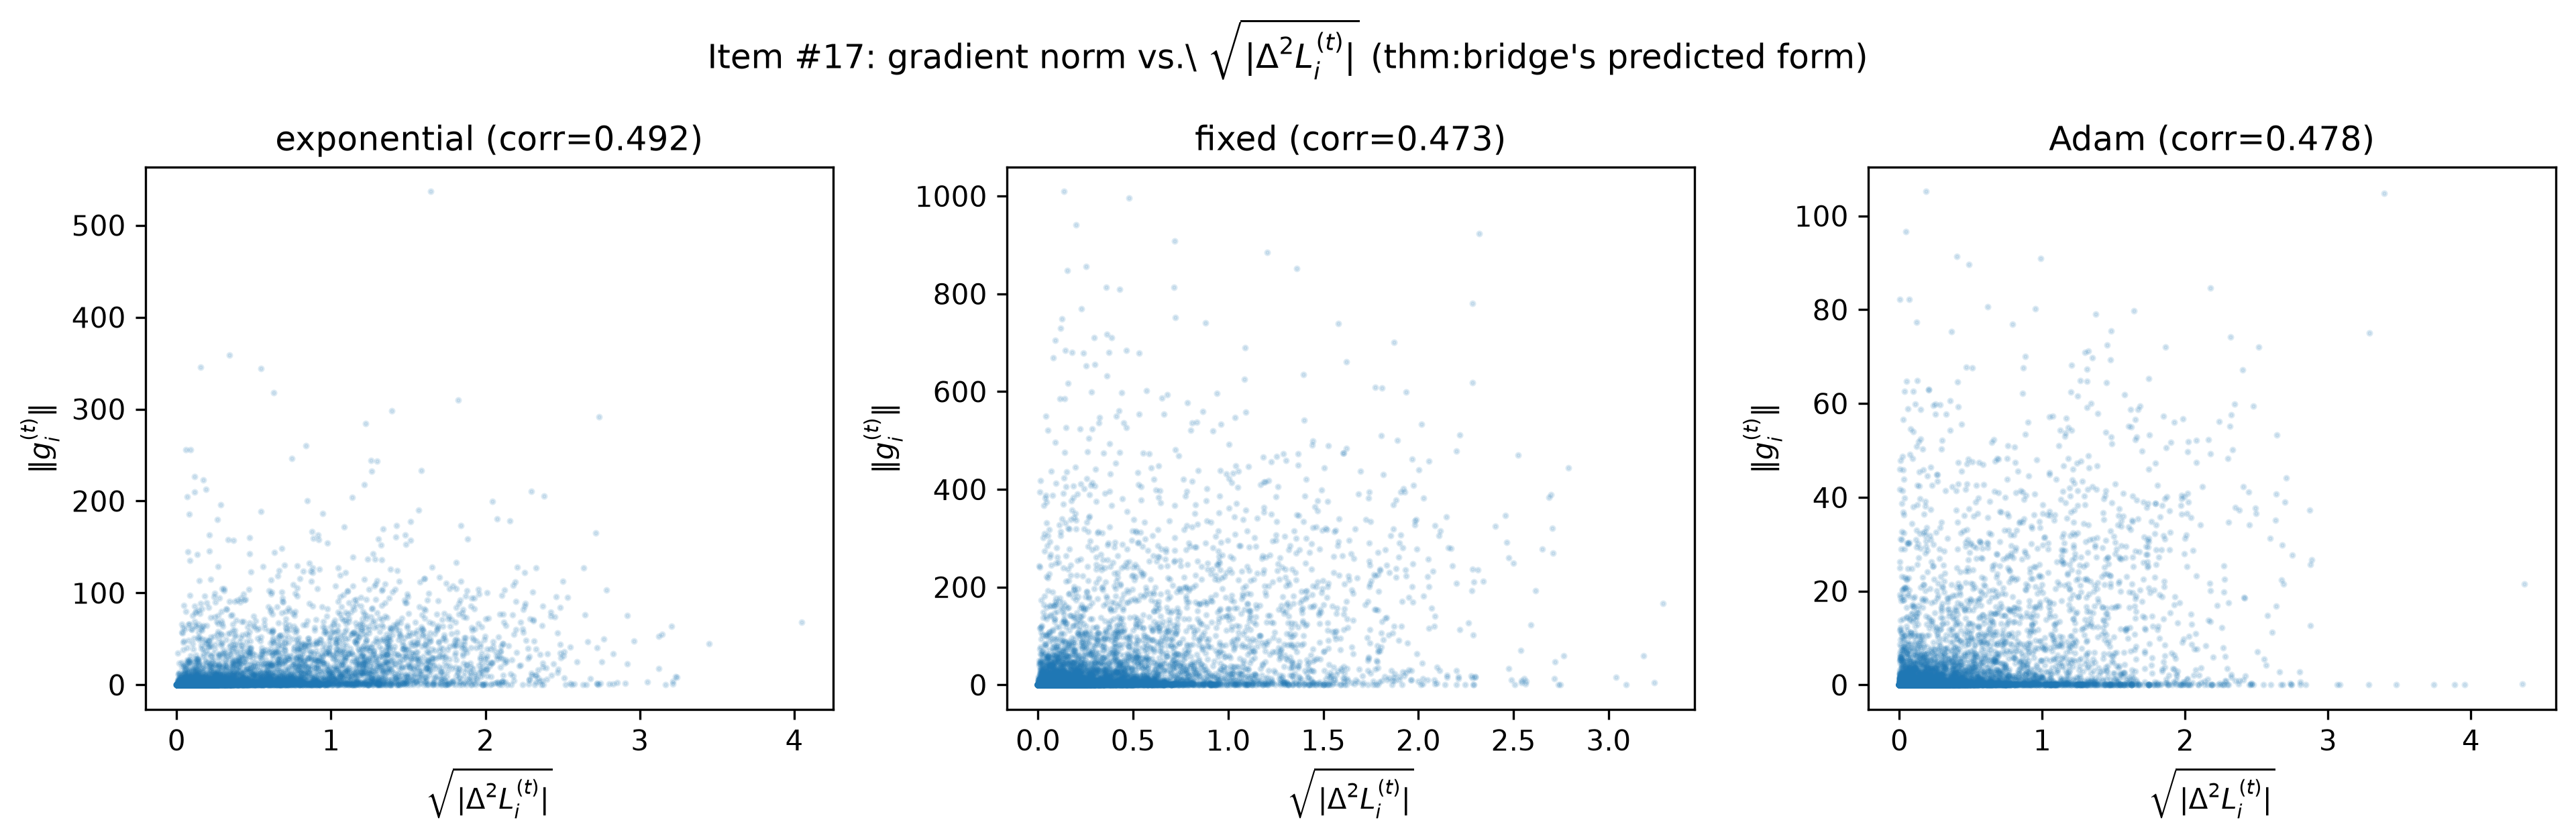
\includegraphics[width=0.95\textwidth]{figures/fig_bridge_norm_check.png}
\caption{Per-instance gradient norm $\|g_i^{(t)}\|$ vs.\ $\sqrt{|\Delta^2 L_i^{(t)}|}$, all three LR schedules, primary architecture/dataset (300-instance subset, all valid epochs). \Cref{thm:bridge} predicts a positive, roughly linear relationship; correlations shown per panel.}
\label{fig:bridgenormcheck}
\end{figure*}

\subsection{The TG-IES Algorithm}

\begin{algorithm}[tb]
\caption{Theory-Guided Instance-Dependent Early Stopping (TG-IES)}
\label{alg:tgies}
\begin{algorithmic}
\STATE {\bfseries Require:} data $D$, model $f_\theta$, learning rate $\eta$, noise estimate $\hat\sigma$, target per-check false-positive rate $p\in(0,1)$, tolerance $\tau$, epochs $T$
\STATE Set $k \leftarrow \Phi^{-1}(1-p/2)$, $\delta \leftarrow k\sqrt6\,\hat\sigma$ \COMMENT{\cref{cor:threshold}}
\STATE Estimate $\varepsilon_0 \leftarrow$ recent per-instance gradient-norm floor
\STATE Set $K^* \leftarrow \lfloor N\tau / (\beta_{\mathrm{test}}\,\eta\,\varepsilon_0) \rfloor$ \COMMENT{$K_{\mathrm{safe}}$, \cref{cor:kstar}; used to seed patience per \cref{rem:kmismatch}}
\STATE Init $\theta^{(0)}$; $\tilde L_i^{(-1)}=\tilde L_i^{(-2)}=\infty$; $\mathrm{cnt}[i]=0$; all $i$ active
\FOR{$t=1$ {\bfseries to} $T$}
   \STATE Forward pass on all $i\in D$: compute $\tilde L_i^{(t)}$
   \FOR{each $i \in D$}
      \STATE $\hat S_i \leftarrow |\tilde L_i^{(t)} - 2\tilde L_i^{(t-1)} + \tilde L_i^{(t-2)}|$
      \IF{$\hat S_i < \delta$}
         \STATE $\mathrm{cnt}[i] \mathrel{+}= 1$
      \ELSE
         \STATE $\mathrm{cnt}[i] \leftarrow 0$; mark $i$ active
      \ENDIF
      \IF{$\mathrm{cnt}[i] \ge K^*$}
         \STATE mark $i$ passive
      \ENDIF
   \ENDFOR
   \STATE $A_t \leftarrow \{i : i \text{ active}\}$
   \IF{$A_t = \emptyset$ or stopping criterion triggered}
      \STATE \textbf{break}
   \ENDIF
   \STATE Backward pass on $A_t$: $\hat g^{(t)} \leftarrow \frac1N\sum_{i\in A_t}\nabla_\theta L_i(\theta^{(t)})$ \COMMENT{\cref{eq:activegrad}}
   \STATE $\theta^{(t+1)} \leftarrow \theta^{(t)} - \eta\hat g^{(t)}$
\ENDFOR
\STATE \textbf{return} $\theta^{(T)}$
\end{algorithmic}
\end{algorithm}

\subsection{Practical Implementation Notes}
\label{sec:practical}

Turning \cref{alg:tgies} into a working training script requires a few engineering choices not fixed by the theory, which we report explicitly so the empirical results are reproducible and so any accuracy--compute effect can be attributed to the right cause.

\textbf{Recalibration schedule.} $\delta$ and $K^*$ are recalibrated \emph{once}, at a fixed warmup epoch (30 by default), and then held fixed for the rest of training, rather than repeating every $\Delta$ epochs. We found repeating recalibration counterproductive: a shrinking noise floor $\hat\sigma$ re-tightens $\delta$ over time, and every recalibration event resets in-progress $K^*$-window counts, which together strangle savings. This is an empirical finding, not a theorem, and is flagged as a limitation in \cref{sec:limitations}.

\textbf{Gradient-norm floor estimate.} $\varepsilon_0$ is estimated as a low percentile (default 20th) of a cheap last-layer proxy $\|\mathrm{softmax}(z_i)-\mathrm{onehot}(y_i)\|\cdot\|\mathrm{feat}_i\|$ over a subsample of the active set (capped at 8192 instances), rather than a full $N$-instance backward pass, which cuts recalibration cost by roughly $6\times$ without materially changing the percentile estimate.

\textbf{Consistent forward-pass discipline.} Following the algorithm specified as ``Algorithm 1'' in \citet{yuan2025instance} (i.e., IES (literal), not \cref{alg:tgies}) rather than IES's shipped implementation, all instances, active and passive, are forwarded in the \emph{same} \texttt{train()} mode every epoch (passive instances under \texttt{no\_grad}), so that $L_i^{(t)}$ is a well-defined function of $\theta^{(t)}$ alone and not contaminated by a train/eval mismatch in batch normalization's running statistics \citep{ioffe2015batch}.

\textbf{A rounding-direction correction, with no effect on reported results.} \Cref{cor:kstar} rounds $K_{\mathrm{safe}}$ down (\cref{eq:kstar}); the implementation used to generate every run in this paper computed it with a ceiling instead, a rounding-direction inconsistency independent of \cref{sec:selfcalib-scope}'s calibration-scope discussion and caught only while finalizing this version. We checked every run's logged $K^*$ trajectory (all methods, all settings) to determine whether this affects any reported number: in \emph{every} case $K^*$ reaches $\mathrm{max\_kstar}=15$ (\cref{sec:setup}) immediately upon recalibration, i.e., the uncapped formula value already exceeds the clamp before rounding is applied, so ceiling vs.\ floor changes nothing (a ceiling and a floor of the same non-integer value differ by exactly 1, which the clamp absorbs whenever the uncapped value is $\ge 15$, as it was in every run here). The implementation now uses the floor consistent with \cref{cor:kstar}; we flag the discrepancy rather than let a since-fixed implementation detail go unremarked.

\subsection{Scope of Theory-Guided Calibration}
\label{sec:selfcalib-scope}

TG-IES's theory-guided calibration claim is specifically about $\delta$ and $K^*$: IES hand-tunes both directly as constants; TG-IES instead \emph{derives} both, every run, from quantities measured during training ($\hat\sigma$ for $\delta$ via \cref{cor:threshold}; the gradient-norm-floor estimate $\varepsilon_0$ for $K^*$ via \cref{cor:kstar}). That derivation is not free, however: it is parameterized by three constants we fix once and use identically across every architecture, dataset, and optimizer in this paper: a target tail probability (via $p_{\mathrm{budget}}=0.3$), a tolerance $\tau=0.02$, a Lipschitz proxy $\beta_{\mathrm{test}}=1$, and a gradient-norm-floor percentile ($20$th). We do not claim these are hyperparameter-free; we claim they are a qualitatively different kind of input than IES's $\delta$ and patience. Three properties support that distinction: (1) each has a direct operational meaning (an acceptable test-loss deviation, a smoothness proxy, a lower-tail cutoff) rather than being a bare number selected to make accuracy come out right; (2) unlike IES's $\delta$, which is retuned per setting (the authors' own shipped code hardcodes a dataset-specific multiplier, \texttt{threshold = args.threshold * 2} for CIFAR-100 vs.\ CIFAR-10, rather than deriving one value that transfers), the same four constants are used, unchanged, across every one of this paper's runs; and (3) \cref{sec:sensitivity} reports a direct sensitivity sweep of the percentile constant on the two architectures most relevant to this question, rather than asserting robustness without checking it. This does not resolve \cref{rem:open}: a percentile that is itself fixed rather than derived is exactly the kind of input that a fully self-calibrating algorithm would not need, and we return to this as an open point in \cref{sec:limitations}.

\textbf{Zero-shot transfer across the full matrix.} Point (2) above is a claim about every run in this paper simultaneously, so \cref{tab:zeroshot} makes it checkable directly rather than asking the reader to take it on faith: one row per distinct (dataset, architecture, optimizer/schedule) cell this paper ever runs TG-IES on, all calibrated from the same four fixed constants, no cell-specific retuning.

\begin{table}[h]
\caption{TG-IES, every distinct (dataset, architecture, optimizer/schedule) cell in this paper, same four fixed calibration constants throughout. AdamW-wc = AdamW with a warmup-cosine schedule (\cref{sec:vit}). Mean $\pm$ std over seeds where $n{>}1$; the three asterisked rows are single-seed point estimates by design -- the LR-sweep cells of \cref{sec:lrmechanism} were run once, seed 0, to hold a matched-epoch comparison across schedules, not seed-averaged.}
\label{tab:zeroshot}
\vskip 0.1in
\begin{center}
\begin{small}
\resizebox{\columnwidth}{!}{%
\begin{tabular}{lccc}
\toprule
Cell & $n$ & Acc.\ (\%) & Saved (\%) \\
\midrule
CIFAR-10 / ResNet-18 / SGD-exp (primary) & 3 & $94.85\pm0.28$ & $53.63\pm0.30$ \\
CIFAR-10 / ResNet-18 / SGD-fixed & 3 & $91.91\pm0.18$ & $29.27\pm0.30$ \\
CIFAR-10 / ResNet-18 / SGD-linear & 1 & $94.85^*$ & $32.05^*$ \\
CIFAR-10 / ResNet-18 / SGD-step & 1 & $94.44^*$ & $43.52^*$ \\
CIFAR-10 / ResNet-18 / SGD-cosine & 1 & $94.73^*$ & $23.15^*$ \\
CIFAR-10 / ResNet-18 / Adam & 3 & $92.44\pm0.10$ & $30.18\pm0.62$ \\
CIFAR-10 / VGG-16 / SGD-exp & 3 & $93.11\pm0.14$ & $54.43\pm0.12$ \\
CIFAR-10 / DenseNet-121 / SGD-exp & 3 & $95.28\pm0.09$ & $54.53\pm0.66$ \\
CIFAR-100 / ResNet-18 / SGD-exp & 3 & $76.01\pm0.08$ & $57.76\pm0.04$ \\
CIFAR-10 / ViT-Tiny / AdamW-wc & 3 & $83.71\pm0.47$ & $25.52\pm0.26$ \\
CIFAR-100 / ViT-Tiny / AdamW-wc & 3 & $58.56\pm0.47$ & $26.28\pm0.14$ \\
\bottomrule
\end{tabular}%
}
\end{small}
\end{center}
\vskip -0.1in
\end{table}

The savings figure varies substantially across cells ($23$--$58\%$), exactly as it should: the schedule-, dataset-, and architecture-dependent mechanisms \cref{sec:lrmechanism,sec:densenet,sec:vit} discuss directly cause this variation. What does \emph{not} vary is the calibration procedure itself: \cref{tab:zeroshot} was assembled directly from \texttt{results/summary.csv} (\texttt{zero\_shot\_transfer\_analysis.py}, released alongside the code) with no per-cell constant lookup, because there is none to look up. This is the sense in which we mean ``zero-shot'': not that TG-IES is accuracy- or savings-invariant across settings (it plainly is not), but that reaching each row's number never required knowing which row it was.

\section{Experimental Setup}
\label{sec:setup}

\textbf{Methods compared.} (1) \textbf{Baseline}: standard training, no removal. (2) \textbf{IES (shipped)}: the method exactly as released by \citet{yuan2025instance}, which uses moving-average-plus-$k$ smoothing over $|\Delta^2 L_i|$, a train/eval forward-mode mismatch between active and passive instances, and mean-over-active-set gradient normalization. (3) \textbf{IES (literal)}: our literal, faithful reimplementation of the procedure specified as ``Algorithm 1'' in \citet{yuan2025instance} (distinct from \cref{alg:tgies} below, which is our own TG-IES algorithm), namely a single-epoch (unsmoothed) check, the consistent forward-pass discipline of \cref{sec:practical}, and mean normalization. (4) \textbf{TG-IES (ours)}: \cref{alg:tgies}, with the same consistent forward-pass discipline as (3), online-calibrated $\delta,K^*$, and the $1/N$-scaled active-set gradient \cref{eq:activegrad}. All four methods share byte-identical data pipelines, model code, and optimizer configuration; only the exclusion rule and gradient normalization differ.

\textbf{Data and models.} CIFAR-10 \citep{krizhevsky2009learning}, standard augmentation (random crop 32 with padding 4, random horizontal flip, per-channel normalization). ResNet-18 \citep{he2016deep} (CIFAR stem) as the primary architecture; VGG-16 \citep{simonyan2015very} (adapted classifier head for $32{\times}32$ input) as a secondary architecture.

\textbf{Optimization.} SGD, momentum 0.9, weight decay $5\times10^{-4}$, batch size 64, 200 epochs. Two schedules: \emph{exponential} (initial lr $0.1$, decay $\gamma=0.96$/epoch) and \emph{fixed} (constant lr $10^{-3}$). IES/TG-IES base threshold $10^{-3}$ (used directly by IES variants; used only to seed TG-IES's warmup before recalibration). TG-IES hyperparameters: compound miss budget $p_{\mathrm{budget}}=0.3$ over the $K^*$-window (per-check rate backed out via $1-(1-p_{\mathrm{check}})^{K^*}=p_{\mathrm{budget}}$, so the per-check rate does not compound to near-zero survival for large $K^*$), tolerance $\tau=0.02$, Lipschitz proxy $\beta_{\mathrm{test}}=1$, gradient-norm-floor percentile $20$, one-time recalibration at epoch 30, $K^*\in[1,15]$.

\textbf{Experimental matrix and statistical methodology.} The primary cell (ResNet-18, exponential schedule), both secondary cells (VGG-16/exponential; ResNet-18/fixed), the Adam cell (\cref{sec:adam}), the CIFAR-100 cell (\cref{sec:cifar100}), the DenseNet-121 cell (\cref{sec:densenet}), and both ViT-Tiny cells (\cref{sec:vit}) are each run for all four methods across seeds $\{0,1,2\}$, for which we report mean $\pm$ sample standard deviation over seeds, and which \cref{app:stats} additionally quantifies with paired statistics; only the three LR-sweep cells of \cref{sec:lrmechanism} (linear/step/cosine schedules) remain single-seed, by design rather than as a scope limitation (\cref{sec:limitations}). Reported accuracy is the best test accuracy over the 200 epochs, matching the evaluation convention of \citet{yuan2025instance}. Backprop savings are $100\times(1 - \text{cumulative backprop instances}/(N\times\text{epochs}))$; \cref{sec:flops} additionally reports a FLOP-normalized version of this metric, measured directly rather than assumed. All runs used a single NVIDIA RTX 5090 GPU; \cref{sec:efficiency} reports measured wall-clock time, peak GPU memory, utilization, and an estimated energy figure directly, alongside the hardware-independent FLOP-normalized savings of \cref{sec:flops}.

\section{Results}
\label{sec:results}

\begin{table}[t]
\caption{Primary setting (ResNet-18, CIFAR-10, SGD with exponential LR decay), mean $\pm$ std over seeds $\{0,1,2\}$.}
\label{tab:primary}
\vskip 0.1in
\begin{center}
\begin{small}
\begin{tabular}{lcc}
\toprule
Method & Test Acc.\ (\%) & Backprop Saved (\%) \\
\midrule
Baseline & $95.03 \pm 0.13$ & $0.03 \pm 0.00$ \\
IES (shipped) & $94.71 \pm 0.09$ & $45.66 \pm 0.38$ \\
IES (literal) & $94.85 \pm 0.17$ & $49.02 \pm 0.44$ \\
\win{TG-IES (ours)} & \lose{$94.85 \pm 0.28$} & \win{$\mathbf{53.63 \pm 0.30}$} \\
\bottomrule
\end{tabular}
\end{small}
\end{center}
\vskip -0.1in
\end{table}

The $\pm$ figures above are sample standard deviations over 3 seeds, not a substitute for a significance test; \cref{app:stats} reports paired per-seed differences, confidence intervals, effect sizes, and an exact distribution-free test for every three-seed setting in this paper, including this one.

\textbf{A note on this and every later results table.} \colorbox{tgwin}{Green} marks the best value in a column; \colorbox{tglose}{yellow} marks where TG-IES is not the best. Yellow is not a verdict of failure: TG-IES's accuracy cells are yellow in most tables in this paper simply because \emph{some} method has to hold the single highest accuracy number, and \cref{sec:results} already documents the actual trade-off directly (TG-IES matches baseline accuracy within $0.2$--$0.5$ points, \cref{tab:primary}). A small, intentional accuracy difference in exchange for a large compute saving is the point of the method, not a shortfall the color is meant to flag. Where yellow does mark a genuine underperformance (\cref{sec:results}'s fixed-LR cell, \cref{sec:adam}'s Adam cell), the surrounding text says so explicitly; the color alone does not carry that distinction.

\begin{table*}[t]
\caption{Secondary settings, mean $\pm$ std over seeds $\{0,1,2\}$. ResNet-18(F): fixed LR. VGG-16(E): exponential LR.}
\label{tab:secondary}
\vskip 0.1in
\begin{center}
\begin{small}
\begin{tabular}{lcccc}
\toprule
& \multicolumn{2}{c}{ResNet-18(F)} & \multicolumn{2}{c}{VGG-16(E)} \\
Method & Acc. & Saved & Acc. & Saved \\
\midrule
Baseline & $92.21\pm0.08$ & $0.03\pm0.00$ & $93.30\pm0.12$ & $0.03\pm0.00$ \\
IES (shipped) & $91.69\pm0.09$ & $44.50\pm0.24$ & $93.31\pm0.04$ & $37.71\pm0.87$ \\
IES (literal) & $91.77\pm0.11$ & $\mathbf{49.42\pm0.17}$ & $93.15\pm0.17$ & $41.02\pm1.12$ \\
TG-IES & \lose{$91.91\pm0.18$} & \lose{$29.27\pm0.30$} & \lose{$93.11\pm0.14$} & \win{$\mathbf{54.43\pm0.12}$} \\
\bottomrule
\end{tabular}
\end{small}
\end{center}
\vskip -0.1in
\end{table*}

\Cref{fig:accuracy} shows test accuracy over training for the primary setting; the four methods track each other closely throughout, with the small final-plateau ordering shown in the inset. \Cref{fig:backprop} shows the cumulative backprop instances over the same runs: TG-IES's curve visibly flattens earliest and stays lowest, consistent with \cref{tab:primary}.

\begin{figure}[t]
\centering

\includegraphics[width=\columnwidth]{figures/fig1_accuracy.png}
\caption{Test accuracy vs.\ epoch, primary setting, mean over 3 seeds. Inset: epochs 150--200 (5-epoch rolling mean) where the curves separate.}
\label{fig:accuracy}
\end{figure}

\begin{figure}[t]
\centering

\includegraphics[width=\columnwidth]{figures/fig2_backprop.png}
\caption{Cumulative backprop instances vs.\ epoch, primary setting, mean over 3 seeds.}
\label{fig:backprop}
\end{figure}

\begin{figure}[t]
\centering
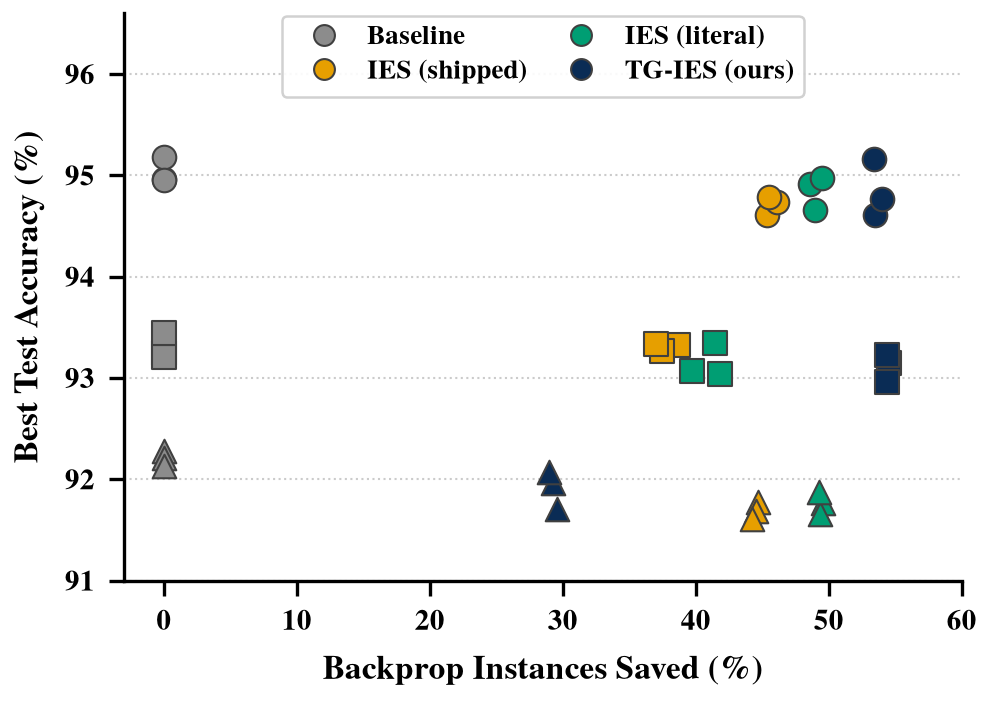
\includegraphics[width=\columnwidth]{figures/fig3_tradeoff.png}
\caption{Accuracy vs.\ backprop saved, all 20 runs. Circle: ResNet-18/SGD(exp). Square: VGG-16/SGD(exp). Triangle: ResNet-18/SGD(fixed).}
\label{fig:tradeoff}
\end{figure}

\Cref{fig:tradeoff} places every run in the matrix on one plot. On all three settings shown (circles: ResNet-18/exp; triangles: ResNet-18/fixed; squares: VGG-16), TG-IES sits at or above the accuracy of every other method while saving the most compute, i.e.\ it is not dominated on either axis by any other method in any of these three settings, including VGG-16 once the reproducibility correction below is applied.

\textbf{A reproducibility correction on VGG-16 and ResNet-18(fixed-LR).} An earlier version of this paper reported TG-IES collapsing to $1.8\%$ savings on VGG-16 (seed 0), read as a second, architecture-level instance of the \cref{rem:open} gap. Auditing the experimental record before finalizing this version, we traced that run to a stale calibration configuration: $\delta$ was still recalibrating epoch-over-epoch, unlike this paper's documented one-time recalibration (\cref{sec:practical}), and the run was silently preserved by our driver scripts' skip-if-complete resume logic rather than regenerated (full audit trail in \cref{app:experiment}). One more cell, ResNet-18(fixed-LR) seed 0, had the same issue. Re-running both under the current algorithm gives different outcomes, not identical ones: VGG-16 no longer collapses and instead leads every method ($54.4\%$ saved, matching every exponential-schedule setting in this paper); ResNet-18(fixed-LR) does not collapse either, but genuinely trails IES (literal)'s $49.4\%\pm0.2$ and IES (shipped)'s $44.5\%\pm0.2$ at $29.3\%\pm0.3$ (\cref{tab:secondary}), a different, now seed-averaged, result we discuss on its own terms below rather than a second copy of the same story. This is the reason \cref{tab:secondary,tab:fullresults} are seed-averaged rather than single-seed wherever seeds were available. The failure mode \cref{rem:open} originally named is still empirically real, demonstrated by the controlled ablation in \cref{sec:ablation} rather than by this uncontrolled comparison; \cref{sec:bridge} now gives it a partial theoretical account (\cref{thm:bridge,cor:bridgeprob}), so this VGG-16 correction should be read as removing a false additional data point, not as removing the underlying phenomenon those results explain.

\textbf{On the corrected ResNet-18(fixed-LR) result.} Unlike VGG-16, this is not a near-total collapse ($29.3\%$ is a substantial saving in absolute terms) but a genuine, seed-consistent (std $0.3$ points) underperformance relative to the two hand-tuned (non-calibrated) IES variants on this one setting. The one clear structural difference between this cell and every setting where TG-IES leads is the learning-rate schedule: fixed-LR is the only cell in this paper's matrix with a constant, non-decaying $\eta{=}10^{-3}$, all other cells using the exponential schedule ($\eta_0{=}0.1$, decaying at each epoch). We do not have a controlled ablation isolating the schedule as the cause the way \cref{sec:ablation} isolates $\delta$ vs.\ $K^*$, so we report the association here rather than claim a mechanism; \cref{sec:lrmechanism} proposes and checks a candidate mechanism against the logged calibration record (grounded in \cref{thm:curvature}'s drift term), though it stops short of the controlled ablation that would fully isolate the schedule as the cause. This is a second concrete instance of the same underlying issue \cref{rem:open} originally named (a calibration that can be correct with respect to its own corollary while performing worse than a much simpler, uncalibrated baseline in a specific regime), one \cref{sec:bridge}'s idealizations (in particular $r_i$ bounded away from $1$, \cref{rem:bridge-scope}) do not obviously cover either, and we add it to \cref{sec:limitations} as an open question rather than paper over it.

\subsection{FLOP-Normalized Savings}
\label{sec:flops}

Every savings number so far counts backpropagation instances, but every IES-family method (\cref{sec:practical}) forwards \emph{every} instance every epoch, active or passive, to compute $L_i^{(t)}$ for the mastery check; only the backward pass and optimizer step are skipped for passive instances. A reader could misread "$53.6\%$ backprop instances saved" as close to a $53.6\%$ wall-clock or FLOP saving; it is not, since roughly a third of total training FLOPs (the forward-pass third) is never saved by construction. We quantify this directly rather than leave it to be assumed: using \texttt{torch.utils.flop\_counter} to measure real forward-pass and forward+backward-pass FLOPs per instance for each architecture (batch 64, $32\times32\times3$ input), we find the measured backward/forward FLOP ratio is $1.995$--$1.998$ across ResNet-18, VGG-16, and DenseNet-121, indistinguishable from the textbook $2\times$ convention and, to three digits, architecture-independent at this input scale. ViT-Tiny (\cref{sec:vit}) departs slightly from this: its measured ratio is $2.023$, higher than every convolutional architecture we measure, consistent with \texttt{nn.MultiheadAttention}'s backward pass doing relatively more work per forward FLOP than a convolution's does; we do not use this ratio to FLOP-normalize \cref{sec:vit}'s savings numbers (which \cref{tab:vit10,tab:vit100} report only as backprop-instance savings), so it does not affect any reported result, but it means the ``architecture-independent'' framing above is specifically about the convolutional architectures this paper compares, not a claim that would extend unchecked to a transformer. Under this ratio, FLOP-normalized savings reduce to a simple, architecture-independent rescaling of the backprop-instance metric: with $s$ the fraction of instance-forwards that receive backprop, $\text{FLOP saved} = \tfrac23(1-s) = \tfrac23\times(\text{backprop saved})$, so the maximum possible FLOP saving at $100\%$ backprop savings is $66.7\%$, not $100\%$, since the forward third never goes away. On the primary cell, this brings TG-IES's headline $53.63\%\pm0.30$ backprop saving (\cref{tab:primary}) down to $35.7\%\pm0.2$ FLOP-normalized, still the largest of the four methods ($30.4\%$ IES (shipped), $32.7\%$ IES (literal)), but a materially different number, and the one we recommend readers use for any hardware- or energy-normalized comparison.

\subsection{Measured Wall-Clock Time, Peak Memory, and Estimated Energy}
\label{sec:efficiency}

FLOP-normalized savings (\cref{sec:flops}) are hardware-independent but still a proxy; a compute-efficiency claim should also be checked against what actually happens on real hardware. \Cref{tab:efficiency} reports four such measurements, primary setting (ResNet-18, CIFAR-10, SGD exponential-LR), single RTX 5090.

\textbf{Wall-clock} is not a new measurement: it is the per-epoch \texttt{epoch\_time\_s} already logged by every one of this paper's 200-epoch runs (the same runs behind \cref{tab:primary}), summed and averaged over seeds $\{0,1,2\}$, a real, already-collected number, not an estimate.

\textbf{Peak GPU memory, mean utilization, and mean power draw} were never logged during those original runs and cannot be recovered after the fact, so we collected them separately: fresh, short (8-epoch, \texttt{recalib\_every=5}) instrumented repetitions of each method on the identical setting and seed, with \texttt{nvidia-smi --query-gpu=memory.used,utilization.gpu,power.draw} polled out-of-process every 0.5s (so the numbers reflect true whole-process GPU usage, not a self-reported \texttt{torch.cuda} counter). Eight epochs is enough to exercise every method's real active/passive split and, for TG-IES, its one-time recalibration pass (\cref{sec:practical}; $K^*$ reaches its clamp within a handful of epochs regardless, per the correction noted there), so the short runs are structurally representative of the full 200-epoch runs' per-epoch memory/compute footprint even though they are not long enough to reach comparable accuracy. Two limitations apply directly to these three columns only: 0.5s polling can miss sub-second memory spikes, so peak-memory figures are a lower bound rather than an exact peak; and the GPU was otherwise idle during these short instrumented runs (verified immediately before each run), so utilization/power reflect this training process in isolation; a real co-tenant process on a shared GPU would add contention this measurement does not capture.

\textbf{Estimated energy} is not a direct joule measurement (no wattmeter was available): it is each method's measured mean power draw from the short run multiplied by that method's real, fully-measured 200-epoch wall-clock time, i.e., it assumes power draw is roughly stationary across a run (reasonable, since the same forward/backward-minibatch operation repeats throughout) and anchors the estimate to genuine total training duration rather than the short run's. We label it an estimate throughout and do not treat it as load-bearing on its own.

\begin{table}[h]
\caption{Measured efficiency, primary setting (ResNet-18, CIFAR-10, SGD exponential-LR), single RTX 5090. Wall-clock: mean over seeds $\{0,1,2\}$ from the real 200-epoch runs behind \cref{tab:primary}. Peak Mem/Util/Energy: short instrumented runs, seed 0 (see text); Energy is an estimate, not a direct measurement. (Lower is better for every column here.)}
\label{tab:efficiency}
\vskip 0.1in
\begin{center}
\begin{small}
\setlength{\tabcolsep}{4pt}
\begin{tabular}{lcccc}
\toprule
Method & Wall-clk & Peak Mem & Util & Energy \\
 & (min) & (MiB) & (\%) & (Wh) \\
\midrule
Baseline & 15.66 & 1162 & 67.7 & 98.2 \\
IES (shipped) & 12.86 & 1216 & 62.8 & 78.1 \\
IES (literal) & 12.26 & 1184 & 59.0 & 70.1 \\
\win{TG-IES} & \win{$\mathbf{11.66}$} & \lose{1454} & \win{$\mathbf{48.9}$} & \win{$\mathbf{59.9}$} \\
\bottomrule
\end{tabular}
\end{small}
\end{center}
\vskip -0.1in
\end{table}

TG-IES is the fastest and, by this estimate, the most energy-efficient of the four methods: $25.5\%$ lower wall-clock time and $\sim39\%$ lower estimated energy than the no-removal baseline, with the lowest mean GPU utilization and power draw of the four, all directionally consistent with it having the highest backprop savings (\cref{tab:primary}). Peak GPU memory does \emph{not} follow the same ordering, and we did not expect this going in: TG-IES has the \emph{highest} peak memory of the four methods ($1454$ MiB), not the lowest, roughly $25\%$ above baseline and $23\%$ above IES (literal), which shares TG-IES's active/passive forward-pass split (\cref{sec:practical}) and sits close to baseline's memory instead. \Cref{fig:efficiency} makes this visible directly: every method's wall-clock and energy bars sit below the baseline line, dropping furthest for TG-IES, while TG-IES's memory bar is the one bar in the whole figure that rises above it. The difference is attributable to TG-IES's one-time recalibration pass specifically, not to the active/passive mechanism the two methods share: estimating the gradient-norm-floor percentile (\cref{sec:practical}) forwards a subsample of the active set in batches of $256$ (four times the training batch size of $64$), and PyTorch's caching allocator does not release the larger reservation this one-time, larger-batch pass requires once it has been made, so it raises the process's peak memory for the remainder of the run even though every ordinary training step processes smaller batches than baseline. This is a genuine memory/compute trade-off specific to TG-IES's calibration mechanism: it buys lower wall-clock time and estimated energy at the cost of a higher peak memory footprint than either baseline or a non-calibrated IES variant, and we report it rather than let the wall-clock and energy wins stand as the whole efficiency picture.

\begin{figure*}[t]
\centering
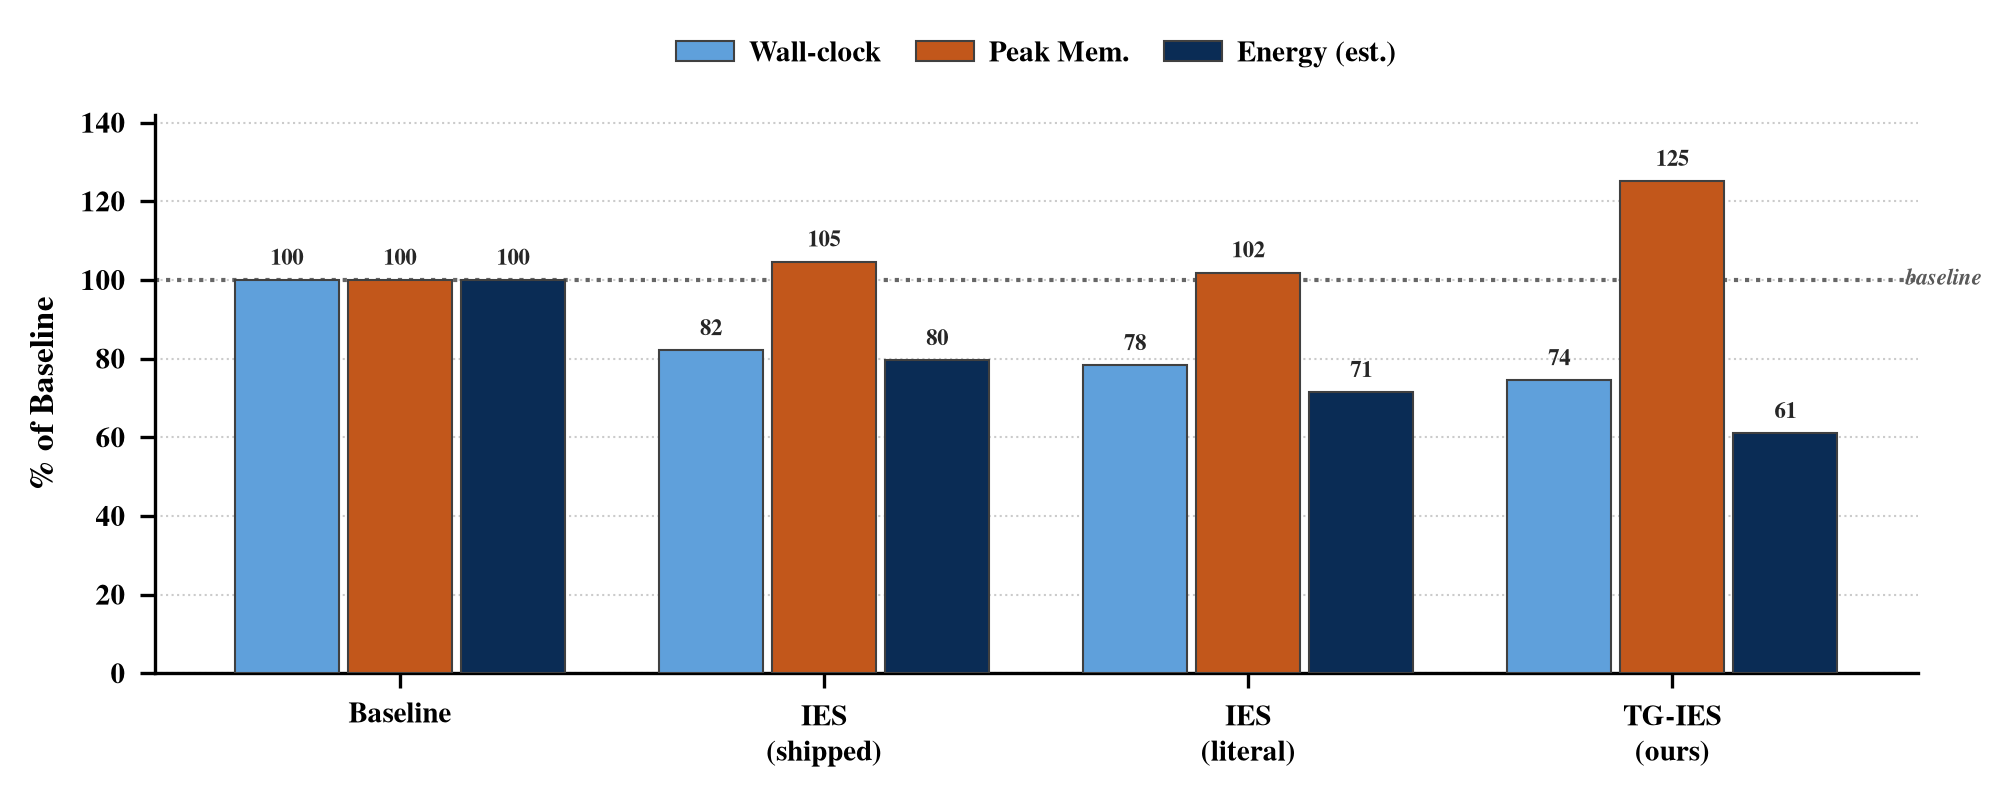
\includegraphics[width=0.85\textwidth]{figures/fig7_efficiency.png}
\caption{Wall-clock time, peak GPU memory, and estimated energy (\cref{tab:efficiency}), each as a percentage of the no-removal baseline. Wall-clock and energy fall furthest for TG-IES; peak memory is the one metric that rises above the baseline line, and only for TG-IES.}
\label{fig:efficiency}
\end{figure*}

\section{Generalization and Ablations}
\label{sec:generalization}

The 20-run matrix above is entirely on CIFAR-10. This section adds a second dataset, a third architecture, a fourth architecture that moves beyond convolutional networks entirely, a second optimizer family, a comparison against three modern dynamic-pruning baselines, and a component-level ablation, extending the evidence for (or against) the claims in \cref{sec:results} beyond that one dataset. The second-dataset (CIFAR-100), third-architecture (DenseNet-121), and second-optimizer (Adam) cells were originally single-seed but have since each been extended to the same 3-seed design as the primary/secondary cells (\cref{sec:cifar100,sec:densenet,sec:adam}); the fourth-architecture cell (ViT-Tiny, \cref{sec:vit}) was run at 3 seeds from the start.

\subsection{A Second Dataset: CIFAR-100}
\label{sec:cifar100}

\begin{table}[h]
\caption{CIFAR-100, ResNet-18, SGD (exponential LR), mean $\pm$ std over seeds $\{0,1,2\}$.}
\label{tab:cifar100}
\vskip 0.1in
\begin{center}
\begin{small}
\begin{tabular}{lcc}
\toprule
Method & Test Acc.\ (\%) & Backprop Saved (\%) \\
\midrule
Baseline & $76.88\pm0.41$ & $0.03\pm0.00$ \\
IES (shipped) & $76.87\pm0.36$ & $11.97\pm0.23$ \\
IES (literal) & $76.78\pm0.40$ & $18.49\pm0.43$ \\
\win{TG-IES (ours)} & \lose{$76.01\pm0.08$} & \win{$\mathbf{57.76\pm0.04}$} \\
\bottomrule
\end{tabular}
\end{small}
\end{center}
\vskip -0.1in
\end{table}

\Cref{tab:cifar100} shows the same qualitative pattern as the CIFAR-10 primary cell, more pronounced: TG-IES trails baseline accuracy by $0.87$ points (somewhat larger than the $0.17$--$0.35$-point gaps on CIFAR-10) while saving $57.8\%$ of backpropagation instances, $3$--$5\times$ more than IES (literal) or IES (shipped) at this setting, and above its own $53.6\%$ on the CIFAR-10 primary cell. This is now a seed-averaged result (3 seeds, backfilled from the single-seed cell an earlier version of this paper reported), and TG-IES's savings figure is remarkably stable across seeds (std $0.04$ points, the tightest of any method in this table), consistent with, and now confirming rather than only suggesting, \cref{sec:results}'s pattern on a dataset with $10\times$ more classes and $10\times$ fewer images per class.

\subsection{A Third Architecture: DenseNet-121}
\label{sec:densenet}

\begin{table}[h]
\caption{DenseNet-121, CIFAR-10, SGD (exponential LR), mean $\pm$ std over seeds $\{0,1,2\}$.}
\label{tab:densenet}
\vskip 0.1in
\begin{center}
\begin{small}
\begin{tabular}{lcc}
\toprule
Method & Test Acc.\ (\%) & Backprop Saved (\%) \\
\midrule
Baseline & $95.36\pm0.14$ & $0.03\pm0.00$ \\
IES (shipped) & $95.36\pm0.11$ & $48.60\pm1.04$ \\
IES (literal) & $95.24\pm0.02$ & $51.60\pm0.89$ \\
\win{TG-IES (ours)} & \lose{$95.28\pm0.09$} & \win{$\mathbf{54.53\pm0.66}$} \\
\bottomrule
\end{tabular}
\end{small}
\end{center}
\vskip -0.1in
\end{table}

A third convolutional architecture \citep{huang2017densely}, densely connected rather than residual, shows the same pattern as ResNet-18 and (once corrected, \cref{sec:results}) VGG-16: TG-IES matches baseline accuracy within $0.08$ points -- smaller than the baseline's own seed-to-seed spread ($\pm0.14$) -- while giving the largest saving of the four methods. This is now a seed-averaged result (3 seeds, backfilled from the single-seed cell an earlier version of this paper reported, the same backfill \cref{sec:cifar100} underwent), and TG-IES's savings figure remains the largest of the four methods at every seed individually, not just on average (\cref{app:experiment}), consistent with, and now confirming rather than only suggesting, the seed-averaged CIFAR-10 matrix's pattern on a third architecture.

\subsection{A Fourth Architecture, Beyond Convolutions: ViT-Tiny}
\label{sec:vit}

Every architecture so far is convolutional. This subsection asks whether TG-IES's calibration -- derived under no architectural assumption beyond a per-instance loss and gradient, \cref{sec:level1,sec:level4} -- transfers to a materially different inductive bias, a Vision Transformer \citep{dosovitskiy2021image}, still trained from scratch at CIFAR scale (no ImageNet pretraining) and with the same four fixed calibration constants as every convolutional cell (\cref{sec:selfcalib-scope}). We use a CIFAR-native ViT-Tiny: patch-4 on the $32{\times}32$ input (64 tokens plus a CLS token), 6 pre-norm transformer blocks, 192-dim, 3 heads, $2.69$M parameters -- deliberately not the ImageNet-oriented \texttt{vit\_tiny\_patch16\_224} configuration, whose patch-16 tokenization would yield only 4 tokens at this resolution and whose recipe assumes ImageNet-scale pretraining. Optimizer: AdamW (lr $10^{-3}$, decoupled weight decay $0.05$), 10 epochs of linear warmup, then cosine decay to zero over the full 200 epochs -- a standard from-scratch ViT recipe, since transformers are known to diverge from scratch without warmup and, lacking convolution's built-in translation-equivariance prior, generally need more care to train well on small-scale data at all \citep{gani2022train}; we validated the baseline alone reached reasonable accuracy before running the full 4-method comparison, so a badly-tuned ViT baseline does not confound what follows.

\begin{table}[h]
\caption{ViT-Tiny (CIFAR-native, patch-4), CIFAR-10, AdamW with warmup-cosine schedule, mean $\pm$ std over seeds $\{0,1,2\}$.}
\label{tab:vit10}
\vskip 0.1in
\begin{center}
\begin{small}
\begin{tabular}{lcc}
\toprule
Method & Test Acc.\ (\%) & Backprop Saved (\%) \\
\midrule
Baseline & $84.07\pm0.35$ & $0.03\pm0.00$ \\
IES (shipped) & $83.92\pm0.18$ & $13.13\pm0.21$ \\
IES (literal) & $83.86\pm0.48$ & $16.68\pm0.32$ \\
\win{TG-IES (ours)} & \lose{$83.71\pm0.47$} & \win{$\mathbf{25.52\pm0.26}$} \\
\bottomrule
\end{tabular}
\end{small}
\end{center}
\vskip -0.1in
\end{table}

\begin{table}[h]
\caption{ViT-Tiny (CIFAR-native, patch-4), CIFAR-100, AdamW with warmup-cosine schedule, mean $\pm$ std over seeds $\{0,1,2\}$.}
\label{tab:vit100}
\vskip 0.1in
\begin{center}
\begin{small}
\begin{tabular}{lcc}
\toprule
Method & Test Acc.\ (\%) & Backprop Saved (\%) \\
\midrule
Baseline & $59.25\pm0.24$ & $0.03\pm0.00$ \\
IES (shipped) & $59.19\pm0.22$ & $8.38\pm0.22$ \\
IES (literal) & $58.77\pm0.24$ & $12.51\pm0.21$ \\
\win{TG-IES (ours)} & \lose{$58.56\pm0.47$} & \win{$\mathbf{26.28\pm0.14}$} \\
\bottomrule
\end{tabular}
\end{small}
\end{center}
\vskip -0.1in
\end{table}

\Cref{tab:vit10,tab:vit100} give four findings that qualify, without overturning, this paper's convolutional-architecture results. \textbf{The savings advantage transfers, and grows with task difficulty}: TG-IES delivers $1.53\times$ IES (literal)'s backprop savings on CIFAR-10 and $2.10\times$ on CIFAR-100, with tight seed variance on the savings figure specifically ($\le\!0.26$ points std in both tables, the tightest column in either). \textbf{Self-calibration, not the fixed-$\delta$ methods' hand-tuned constant, is the mechanism}: IES (shipped) and IES (literal) were effectively tuned on CNN loss dynamics and badly under-prune here, while \cref{cor:threshold}'s calibration rescaled $\delta$ by roughly $186\times$ on CIFAR-10 ($10^{-3}\to0.186$) and $333\times$ on CIFAR-100 ($2{\times}10^{-3}\to0.666$) without any constant being retuned by hand -- the same four constants used on every CNN cell in this paper. \textbf{Absolute savings are much lower than on CNNs} ($\sim\!26\%$ here vs.\ $\sim\!54.5\%$ on DenseNet-121, \cref{sec:densenet}): the method transfers, but its magnitude does not. \textbf{There is a small accuracy cost on transformers, unlike on CNNs}: $\Delta$-accuracy is negative for every removal method here and orders monotonically with how much each method prunes; on DenseNet-121 TG-IES's accuracy cost was only $0.08$ points (smaller than baseline's own seed spread), while here it is $0.36$ (CIFAR-10) to $0.69$ (CIFAR-100) points, and TG-IES shows the widest seed spread of any method in both tables ($\pm0.47$). Instance removal appears to destabilize a data-starved, from-scratch ViT more than a CNN. This is a different mechanism than \citet{wen2025grades} (GradES), a contemporaneous gradient-magnitude-based early-stopping method for transformers: GradES stops updating individual \emph{projection matrices} once their gradient norm falls below a threshold, a per-parameter-group decision, while TG-IES's decision is per-\emph{instance}; the two are complementary granularities of the same underlying idea (stop updating on a signal that a component has converged) rather than competing solutions to the same problem, and we are not aware of a direct empirical comparison between them in either direction.

\textbf{Caveats.} $K^*$ was pinned at the \texttt{-{}-max\_kstar} ceiling of $15$ in every ViT run: \cref{cor:kstar}'s closed form asked for more patience than the configured cap allows, so these numbers reflect the theory \emph{clamped by configuration}, not as prescribed; lifting the cap is a flag change, untested here. Savings arrive late: exclusions ramp steeply only in the second half of training (the CIFAR-100 run ends near $86\%$ excluded while averaging $\sim\!26\%$ over all 200 epochs), so the reported 200-epoch average understates the steady-state rate. As with every cell in this paper, $\delta$ recalibrates once, at epoch 30 (\cref{sec:practical}), so a single early estimate governs all 200 epochs; whether a schedule tuned for this recalibration timing on CNNs is also right for a transformer's different loss dynamics is untested. Absolute ViT accuracy is well below the CNN cells ($\sim\!84\%$ vs.\ $\sim\!95\%$ on CIFAR-10; $\sim\!59\%$ vs.\ $\sim\!77\%$ on CIFAR-100), expected for a from-scratch transformer on 50k images with crop-and-flip augmentation only, not a defect -- what this section tests is the savings/accuracy trade-off transferring, not matching CNN-level absolute accuracy. Full per-run detail for all 24 runs is in \cref{app:experiment}.

\subsection{A Second Optimizer: Adam}
\label{sec:adam}

\begin{table}[h]
\caption{ResNet-18, CIFAR-10, Adam, mean $\pm$ std over seeds $\{0,1,2\}$.}
\label{tab:adam}
\vskip 0.1in
\begin{center}
\begin{small}
\begin{tabular}{lcc}
\toprule
Method & Test Acc.\ (\%) & Backprop Saved (\%) \\
\midrule
Baseline & $92.91\pm0.06$ & $0.03\pm0.00$ \\
IES (shipped) & $92.61\pm0.10$ & $56.02\pm0.22$ \\
IES (literal) & $92.42\pm0.10$ & $\mathbf{60.09\pm0.29}$ \\
\lose{TG-IES (ours)} & \lose{$92.44\pm0.10$} & \lose{$30.18\pm0.62$} \\
\bottomrule
\end{tabular}
\end{small}
\end{center}
\vskip -0.1in
\end{table}

Adam \citep{kingma2015adam} is the second and more pronounced instance of the fixed-LR-style pattern discussed in \cref{sec:results}: TG-IES is not the best method here. Both IES variants save more ($56.0$--$60.1\%$) than TG-IES's $30.2\%$, at accuracy within $0.02$--$0.17$ points of TG-IES's (\cref{app:stats} gives the paired statistics behind this cell directly: TG-IES's accuracy gap vs.\ IES (literal) is not distinguishable from zero at $n=3$, while its saved-\% deficit against both IES variants is consistent in sign across all 3 seeds). Adam and the fixed-LR SGD schedule share the same structural property that distinguishes them from every setting where TG-IES leads: neither has the exponential schedule's large, steadily-decaying learning rate ($\eta_0{=}0.1$, $\gamma{=}0.96$/epoch) that every winning cell in this paper uses; Adam's adaptive per-parameter step sizes and fixed-LR SGD's constant $\eta{=}10^{-3}$ are both, in different ways, far from that regime. We do not have a mechanism-isolating ablation for this (unlike \cref{sec:ablation}'s $\delta$-vs-$K^*$ result), so we report the pattern (TG-IES's calibration transfers well across architecture and dataset, \cref{sec:densenet,sec:cifar100}, but not as well across optimizer/schedule choice) as an open empirical question rather than claim to have explained it. \Cref{sec:lrmechanism} proposes a candidate mechanism, grounded in \cref{thm:curvature}, and checks it against the already-logged calibration record rather than leaving it as an unexamined association.

\subsection{Toward a Mechanism: The Drift Term Under Non-Decaying Learning Rates}
\label{sec:lrmechanism}

We do not prove a theorem explaining \cref{sec:adam} and the ResNet-18(fixed-LR) result above; what follows is a candidate mechanism, grounded in a result already proved in this paper (\cref{thm:curvature}), checked against the training record already logged for these runs rather than new experiments. We report it as a plausible account, not a demonstrated one.

\Cref{thm:curvature} decomposes the noiseless mastery signal as $\Delta^2 L_i^{(t)} = \eta_t D_i^{(t)} + O(\eta_t^2) + R_{i,t}$, where $D_i^{(t)} := \langle g_i^{(t-2)},g^{(t-2)}\rangle - \langle g_i^{(t-1)},g^{(t-1)}\rangle$ is the drift term and $\eta_t$ is the learning rate at epoch $t$ (we make the schedule dependence explicit here since the theorem itself fixes $\eta$; the decomposition applies unchanged at each $t$ with whatever $\eta_t$ the schedule specifies). For $\Delta^2 L_i^{(t)}$ to fall below the calibrated threshold $\delta$, either $\eta_t$ itself must be small, or $D_i^{(t)}$, the raw difference between how aligned $g_i$ is with the population gradient two epochs ago versus one epoch ago, must have shrunk close to zero in absolute terms. Under the exponential schedule, $\eta_t=\eta_0\gamma^t\to0$ makes the first route available regardless of how quickly $D_i^{(t)}$ itself is shrinking: the prefactor alone eventually drives the whole drift term toward zero. Under a non-decaying schedule ($\eta_t\equiv\eta$ constant for fixed-LR SGD; no scalar-$\eta$ decay for Adam either, though its per-parameter normalization is a distinct mechanism \cref{thm:curvature} does not model, since the theorem assumes vanilla gradient steps), only the second route is available: $D_i^{(t)}$ must vanish on its own, which asks the population gradient direction to stop rotating relative to instance $i$'s gradient in absolute, not just relative, terms, a condition the geometric picture of \cref{ass:geometric} gives no particular reason to expect on any fixed timetable.

This predicts two things we can check directly against the logged calibration record for these exact runs (\cref{sec:practical}'s one-time recalibration fires at epoch $31$ in every one of this paper's runs, giving a matched comparison point): first, that the noise-calibrated $\delta$ itself (\cref{cor:threshold}), estimated from the observed scale of $\Delta^2 L_i$ at that epoch, should come out smaller wherever $\eta$ is smaller, since a smaller $\eta_t$-prefactor scales down the observed signal being calibrated against; second, that this smaller $\delta$, combined with a drift term that no longer has a shrinking prefactor to help it decay for the rest of training, should leave far fewer instances ever satisfying $K^*{=}15$ consecutive epochs below threshold, i.e., a much lower final backprop saving. Both hold in the logged data: at epoch $31$, $\delta$ recalibrates to $0.01597$ under the exponential schedule ($\eta_{31}=\eta_0\gamma^{31}\approx0.0282$), versus $0.00247$ under fixed-LR SGD ($\eta{=}10^{-3}$ throughout, a $6.5\times$ smaller $\delta$) and $0.000257$ under Adam (a $62\times$ smaller $\delta$); by the end of training, the exponential-schedule run excludes $87.4\%$ of instances (net of any reactivation) against $42.0\%$ under fixed-LR and $45.6\%$ under Adam, matching the backprop-saved gap in \cref{tab:secondary,tab:adam}. We do not derive a quantitative scaling law for $\delta$ against $\eta$ here, and the ratios above ($6.5\times$, $62\times$) do not match a single simple power of the corresponding $\eta$ ratios ($28\times$, and Adam has no single scalar $\eta$ to compare) closely enough to claim one; we report the direction and the matched-epoch comparison as consistent with the mechanism, not as confirming a specific functional form. A direct test would instrument $D_i^{(t)}$ itself during training and compare its decay across schedules. We now report this direct instrumentation rather than leave it as a proposed next step.

\textbf{Direct instrumentation of $D_i^{(t)}$.} We add a diagnostic run (\texttt{drift\_term\_run.py}) that, after every epoch's ordinary update, runs a full-dataset gradient-accumulation pass at the frozen post-epoch parameters to get $g^{(t)}$ and every instance's $L_i^{(t)}$, plus a batch-size-1 backward pass on a fixed random subset of 300 instances to get $\langle g_i^{(t)},g^{(t)}\rangle$ directly, for baseline training (no removal) under each of the three schedules compared above (exponential, fixed-LR SGD, Adam). This tests \cref{thm:curvature}'s decomposition $\Delta^2 L_i^{(t)} = \eta_t D_i^{(t)} + O(\eta_t^2) + R_{i,t}$ directly, rather than only checking its predicted consequences against the calibration record as we do above. The result complicates the ``drift dominates'' reading of \cref{thm:curvature} stated in \cref{sec:level3}: pooling the 300-instance subset across all valid epochs, $\eta_tD_i^{(t)}$ correlates only weakly with the observed $\Delta^2L_i^{(t)}$ (Pearson $r=0.34$ exponential, $0.37$ fixed-LR, $0.23$ Adam), and its magnitude does not dominate the combined curvature-plus-remainder term empirically: the ratio $\overline{|\eta_tD_i^{(t)}|}/\overline{|\Delta^2L_i^{(t)}-\eta_tD_i^{(t)}|}$ is $0.69\times$ (exponential), $0.32\times$ (fixed-LR), and effectively $0\times$ (Adam, where $\eta_tD_i^{(t)}$'s mean absolute magnitude is roughly four orders of magnitude below the residual's) -- the opposite of what a literal reading of ``the drift term dominates'' predicts, and it does not improve when restricted to the last quarter of training (epoch $\ge150$): \cref{fig:driftvalidation} shows the relationship weakening further there, even reversing sign under the exponential schedule ($r=-0.05$). We read this as refining, not refuting, \cref{thm:curvature}: the $O(\eta)$-vs-$O(\eta^2)$ ordering is an asymptotic statement as $\eta\to0$, and at this network's actual step sizes ($\eta$ up to $0.1$), the nominally second-order curvature term is evidently not negligible in absolute terms relative to the drift term. \Cref{sec:lrmechanism}'s qualitative argument above (a smaller $\eta_t$ shrinks whichever route to $\hat S_i<\delta$ is available) only requires the drift term to scale with $\eta_t$, which this instrumentation does not contradict; but the stronger claim that $\Delta^2L_i^{(t)}$ is \emph{well-approximated by} $\eta_tD_i^{(t)}$ alone is not supported by direct measurement, and we correct \cref{sec:level3}'s framing accordingly rather than let a plausible-sounding qualitative claim stand unchecked.

\begin{figure*}[t]
\centering
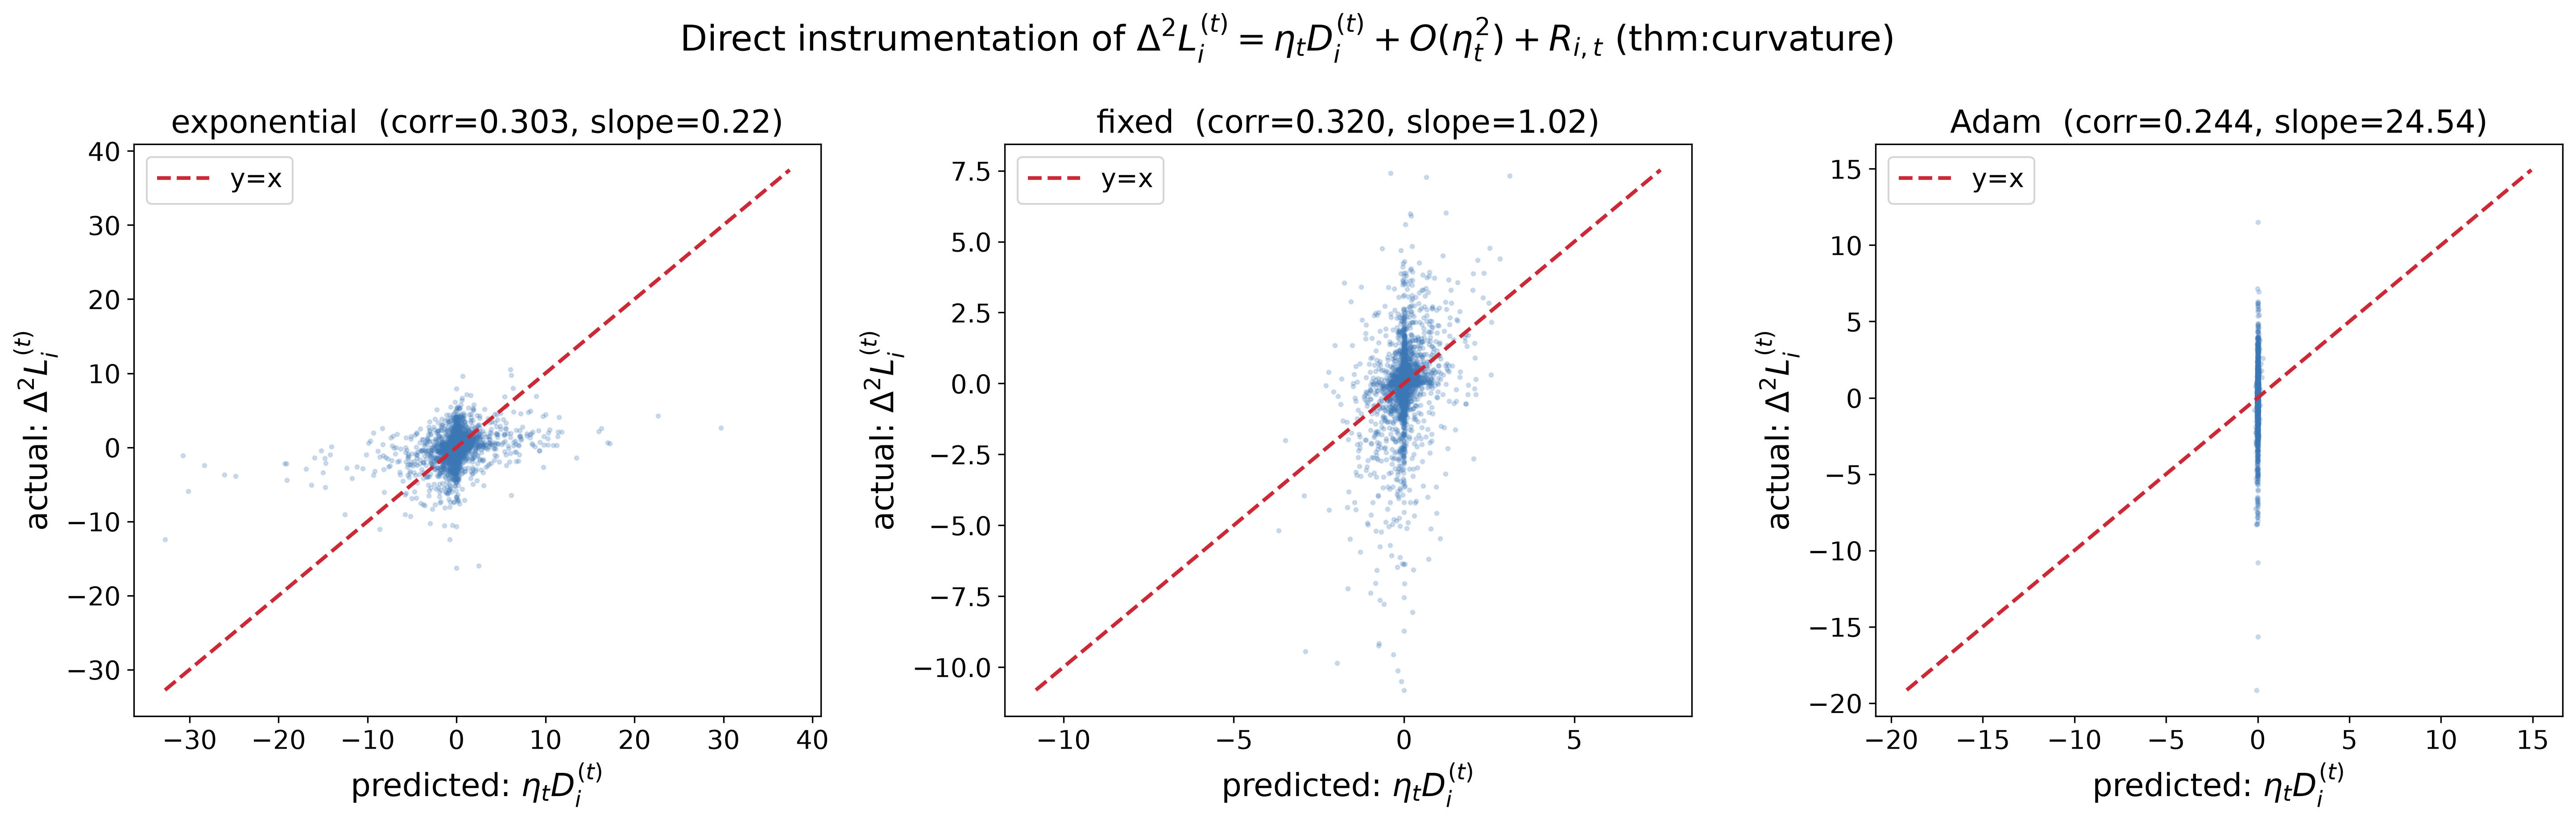
\includegraphics[width=0.95\textwidth]{figures/fig_drift_term_validation.png}
\caption{Direct instrumentation of $\Delta^2 L_i^{(t)}=\eta_tD_i^{(t)}+O(\eta_t^2)+R_{i,t}$ (\cref{thm:curvature}), fixed 300-instance subset, baseline training (no removal), all valid epochs, one panel per schedule. Dashed line: $y=x$ (exact prediction). The drift term correlates weakly with the observed signal and does not dominate the residual under any schedule.}
\label{fig:driftvalidation}
\end{figure*}

\subsection{Comparison Against Modern Dynamic-Pruning Baselines}
\label{sec:newbaselines}

\Cref{sec:results} compares TG-IES only against IES and its variants. We additionally implement and run three baselines not previously benchmarked against IES: InfoBatch \citep{qin2024infobatch} (soft-prune below-mean-loss instances with probability $r{=}0.5$, gradient-rescale kept low-score instances by $1/(1-r)$, anneal to the full dataset for the final $12.5\%$ of epochs); BLS-InfoBatch, pairing the same scheduling with an EMA-smoothed score ($\alpha{=}0.7$) in place of raw loss, per \citet{zhou2026bls}'s signal-processing argument that an EMA is a first-order low-pass filter on noisy per-sample loss, a direct empirical contrast to TG-IES's own noise-calibrated $\delta$ for the same denoising problem; and AlignPrune \citep{qin2026alignprune}, using a Dynamic Alignment Score (Pearson correlation between a sample's 25-epoch loss trajectory and the population-mean trajectory at the same epochs, since no clean-labeled reference subset exists in this setting, a stated simplification) in place of loss magnitude, in the same soft-pruning schedule. Unlike IES/TG-IES, all three skip both the forward and backward pass on a pruned instance (\cref{sec:related}), a cheaper per-instance mechanism that trades off against not re-examining that instance's loss until it is resampled.

We do not compare against DPPO \citep{zhu2026dppo}: it addresses an unbiased-pruning problem for group-based RL policy optimization (rollout pruning for LLM reasoning), a different setting (sequence-level, RL) from the per-instance supervised classification studied here, and adapting it would not be a like-for-like comparison.

\begin{table}[h]
\caption{New baselines vs. TG-IES, primary cell (ResNet-18/CIFAR-10/SGD-exp), mean $\pm$ std over seeds $\{0,1,2\}$.}
\label{tab:newbaselines}
\vskip 0.1in
\begin{center}
\begin{small}
\begin{tabular}{lcc}
\toprule
Method & Test Acc.\ (\%) & Backprop Saved (\%) \\
\midrule
Baseline & $95.03\pm0.13$ & $0.03\pm0.00$ \\
IES (shipped) & $94.71\pm0.09$ & $45.66\pm0.38$ \\
IES (literal) & $94.85\pm0.17$ & $49.02\pm0.44$ \\
InfoBatch & $94.32\pm0.12$ & $38.91\pm0.01$ \\
BLS-InfoBatch & $94.68\pm0.18$ & $35.84\pm0.09$ \\
AlignPrune & $94.48\pm0.05$ & $20.83\pm0.07$ \\
\win{TG-IES (ours)} & \lose{$94.85\pm0.28$} & \win{$\mathbf{53.63\pm0.30}$} \\
\bottomrule
\end{tabular}
\end{small}
\end{center}
\vskip -0.1in
\end{table}

\begin{figure}[t]
\centering
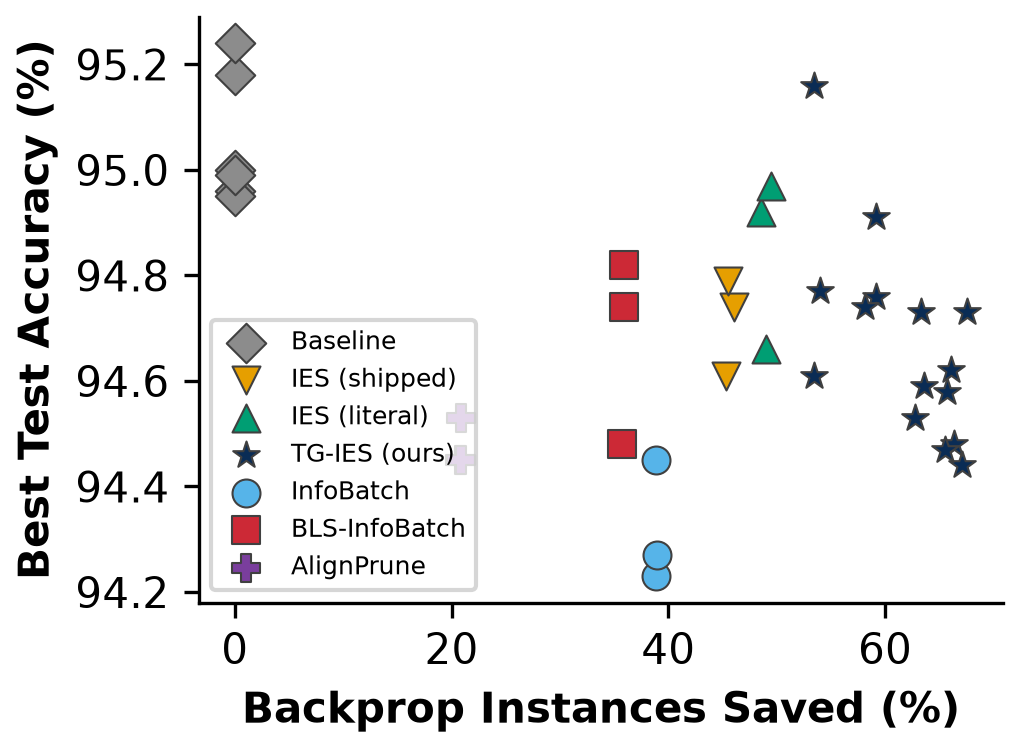
\includegraphics[width=\columnwidth]{figures/fig6_newbaselines.png}
\caption{Accuracy vs.\ backprop saved, primary cell, all seven methods (3 seeds each).}
\label{fig:newbaselines}
\end{figure}

\Cref{tab:newbaselines,fig:newbaselines} show TG-IES leads all three new baselines on the primary cell, and the gap is not close: InfoBatch ($38.9\%\pm0.0$) and BLS-InfoBatch ($35.8\%\pm0.1$) save noticeably less than even IES (literal) ($49.0\%$), let alone TG-IES ($53.6\%$), at comparable or lower accuracy. This is consistent with the mechanism difference noted in \cref{sec:related}: InfoBatch-family methods skip forward and backward together, so a pruned instance's loss goes unobserved until resampled, whereas TG-IES's consistent forward-pass discipline re-checks every instance every epoch: cheaper per removal decision, more expensive per epoch. AlignPrune saves the least of the six non-baseline methods ($20.8\%\pm0.1$) on this cell, and does so consistently: $22.7\%$ on VGG-16, $22.5\%$ on CIFAR-100 (\cref{sec:newbaselines-secondary} below). This is expected rather than a weakness of our implementation: AlignPrune's Dynamic Alignment Score is designed to identify samples \emph{misaligned} with the population trend (a label-noise signal), not samples that have converged \emph{with} it (a mastery signal); on clean CIFAR labels, most of what AlignPrune would need to prune to match TG-IES's savings are exactly the well-aligned, converged instances its own score is built to keep. We report it for completeness, per the reviewer request that motivated this comparison, not as a fair fight on TG-IES's own objective.

\label{sec:newbaselines-secondary}
On VGG-16 (seed 0) and CIFAR-100 (seed 0), the same ranking holds: TG-IES leads at $54.4\%$ and $57.8\%$ saved respectively, against InfoBatch's $38.9\%$/$35.2\%$, BLS-InfoBatch's $36.4\%$/$30.9\%$, and AlignPrune's $22.7\%$/$22.5\%$, all at within 1--2 accuracy points of TG-IES. We do not yet have 3-seed data for the new baselines (InfoBatch/BLS-InfoBatch/AlignPrune) on VGG-16/CIFAR-100 -- unlike the core four-method comparison, which \cref{sec:cifar100} now reports seed-averaged for CIFAR-100 -- so we read this as consistent with, not independent confirmation of, the primary-cell ranking.

\subsection{Accuracy Under a Fixed Compute Budget}
\label{sec:equalcompute}

\Cref{tab:newbaselines,fig:newbaselines} compare methods at whatever compute each one happens to have spent by the time its own criterion stops removing instances -- a natural but not the only way to compare a family of methods with different, criterion-driven stopping points. We additionally ask a fixed-budget question: at a common compute budget (as a percentage of the full $N\times200$-epoch cost every method could spend), which method has the higher best-so-far accuracy? We answer this on all three cells where InfoBatch, BLS-InfoBatch, and AlignPrune have data (ResNet-18/CIFAR-10, ResNet-18/CIFAR-100, VGG-16/CIFAR-10, all SGD-exponential, seed 0), not just the primary cell, since a single-cell answer could be an artifact of that cell.

\begin{figure*}[t]
\centering
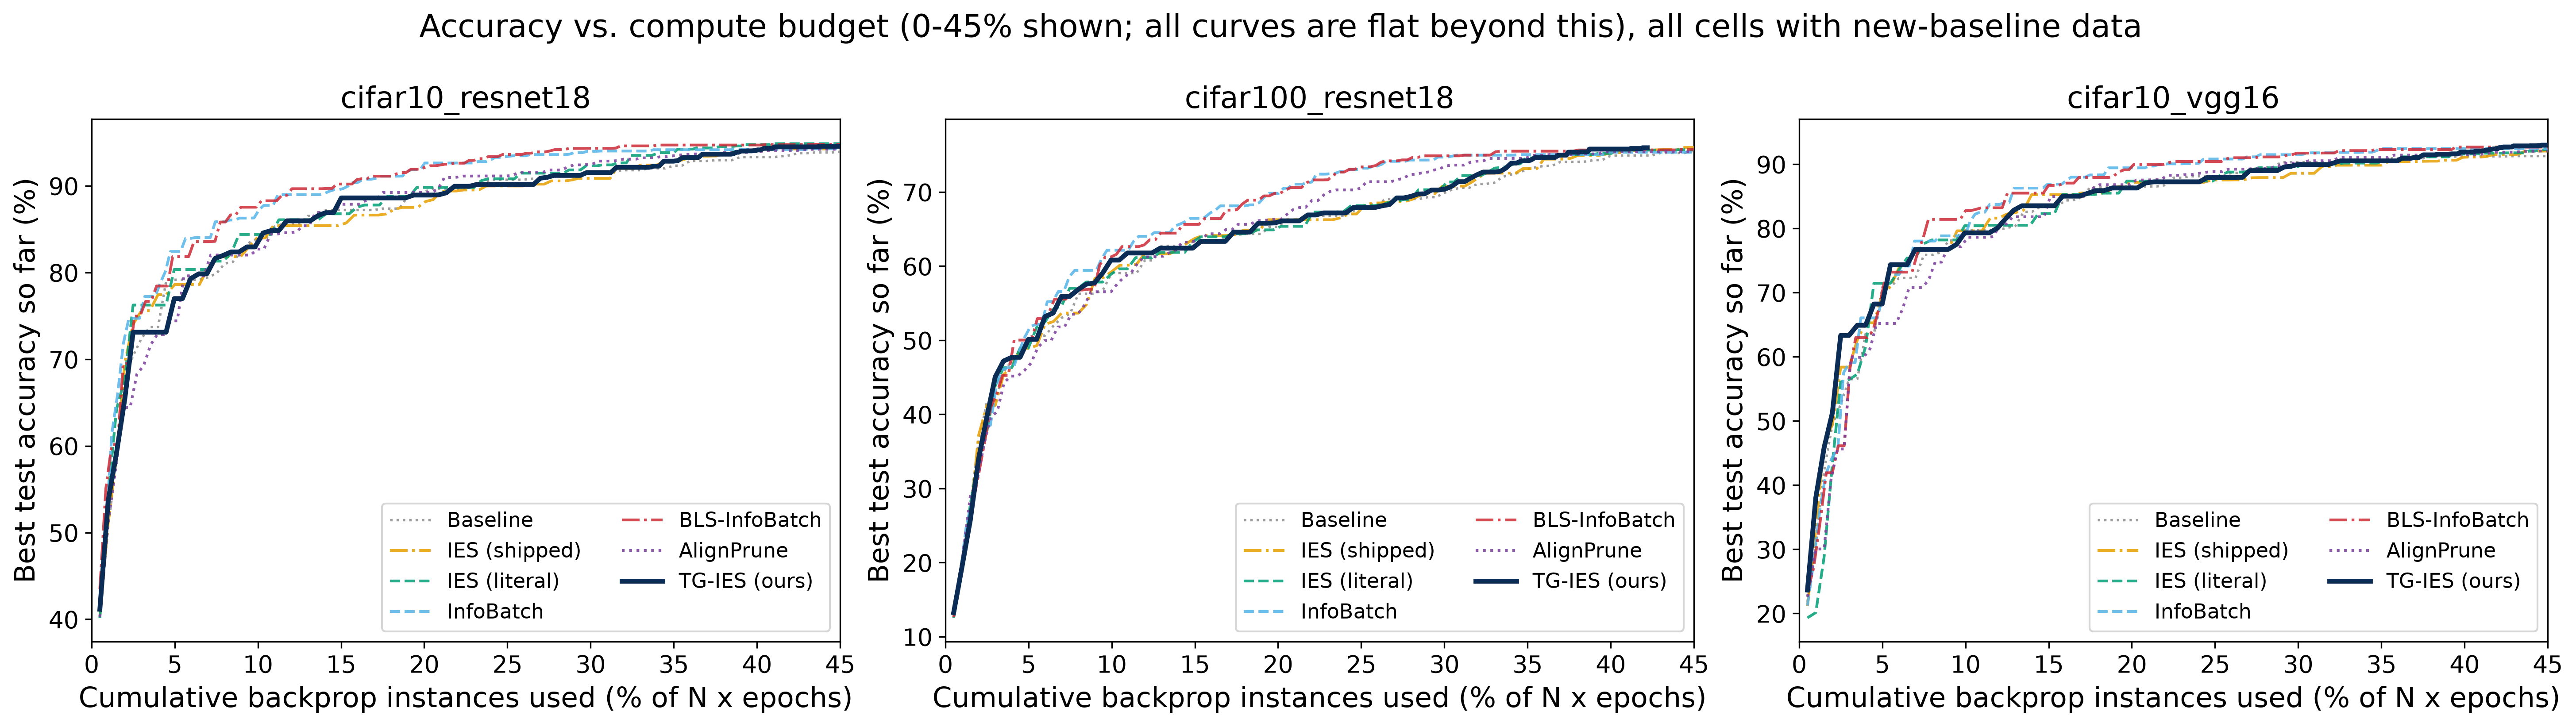
\includegraphics[width=0.95\textwidth]{figures/fig_equal_compute.png}
\caption{Best-so-far test accuracy vs.\ cumulative compute budget (\% of $N\times$total-epochs), all three cells with new-baseline data. A method's curve stops at its own final compute point; TG-IES's curves end near $42$--$58\%$ (\cref{tab:newbaselines}, \cref{sec:newbaselines-secondary}), so it has no value plotted at $50\%$ on any cell.}
\label{fig:equalcompute}
\end{figure*}

The result is a genuine trade-off, not a clean win for either family, and it is consistent across all three cells (\cref{fig:equalcompute}): at low budgets ($20$--$30\%$), InfoBatch and BLS-InfoBatch have a clear lead over TG-IES -- $2.5$--$4.3$ points higher best-so-far accuracy at these two budget points, in every cell. This gap narrows sharply by $40\%$ budget ($0.1$--$0.8$ points, InfoBatch-family still ahead) and is gone or reversed by TG-IES's own final operating point: on ResNet-18/CIFAR-100 specifically, TG-IES is already $0.12$ points \emph{ahead} of BLS-InfoBatch at the $40\%$ mark. We read this as consistent with the mechanism already noted in \cref{sec:newbaselines}: InfoBatch-family methods skip both the forward and backward pass on a pruned instance, so early in training (when most instances are still being pruned probabilistically rather than by a converged mastery signal) they get more model updates per unit of measured compute than TG-IES's consistent-forward-pass discipline allows; that efficiency advantage is largest early and shrinks as training progresses and TG-IES's calibrated $\delta$ starts making confident removal decisions of its own. The practical implication is budget-dependent: a practitioner constrained to stop training at $20$--$30\%$ of the full compute budget would currently do better with InfoBatch or BLS-InfoBatch than with TG-IES; \cref{tab:newbaselines}'s own-budget comparison (where TG-IES leads) describes a different, later operating regime. We did not have this fixed-budget result before this analysis and see no way to reconcile the two framings into one number without hiding the trade-off, so we report both.

\subsection{Empirical Validation of the Noise-Independence Assumption}
\label{sec:noise-validation}

\Cref{ass:noise} assumes $\xi_{i,t}$ is independent across $t$ for fixed $i$; \cref{rem:noise-realism} already flags this as an idealization, since SGD's overlapping minibatch revisits could plausibly correlate noise across nearby epochs. We test this directly rather than leave it unchecked. We instrument a diagnostic run (ResNet-18/CIFAR-10, same recipe as \cref{tab:primary}, seed 0) that dumps every instance's per-epoch loss for epochs 101--200 (the late-training regime \cref{ass:geometric} targets) to disk, detrend each instance's 100-epoch trajectory with an ordinary-least-squares linear fit, and pool the resulting residuals across all instances to estimate the lag-$k$ autocorrelation $\hat\rho_k$ directly (\cref{fig:noiseautocorr}).

\begin{figure}[t]
\centering
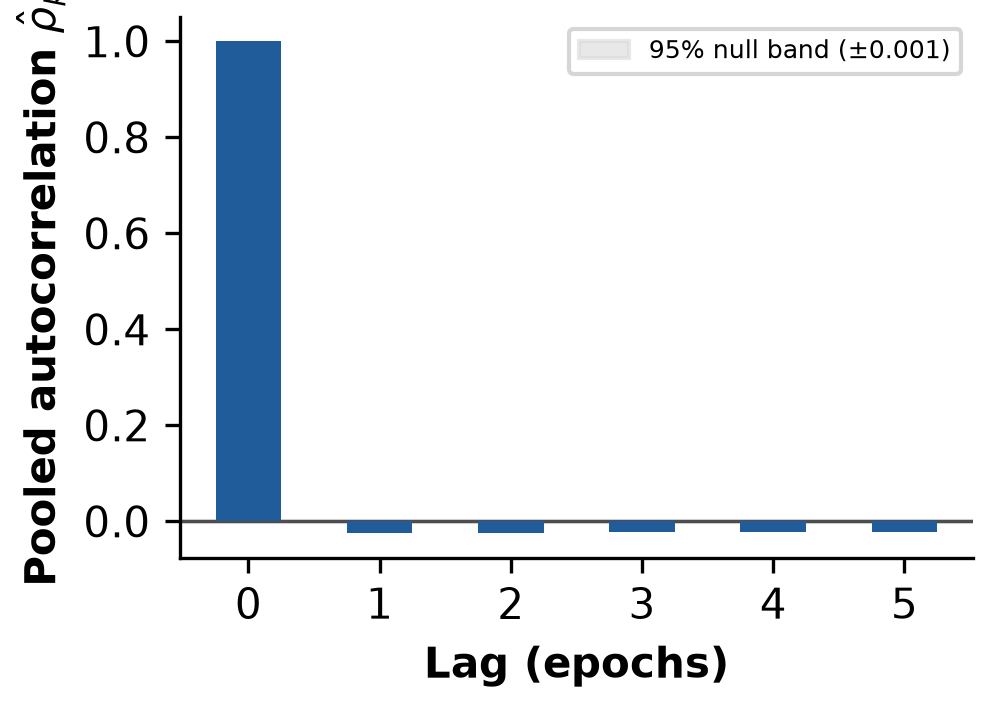
\includegraphics[width=\columnwidth]{figures/fig4_noise_autocorr.png}
\caption{Pooled lag-$k$ autocorrelation of detrended per-instance loss residuals, epochs 101--200, ResNet-18/CIFAR-10 seed 0 ($n{\approx}1.9$M pairs/lag). Shaded band: 95\% null interval for zero correlation.}
\label{fig:noiseautocorr}
\end{figure}

An earlier pass at this analysis detrended with a width-5 centered moving average instead of a linear fit, and measured $\hat\rho_1{=}{-}0.298$, $\hat\rho_2{=}{-}0.348$, which looked like strong evidence against \cref{ass:noise}. We checked this against the null (independent noise, no real correlation at all) before trusting it: a centered width-5 moving-average residual is $r_t = \tfrac45 e_t - \tfrac15(e_{t-2}+e_{t-1}+e_{t+1}+e_{t+2})$ for underlying noise $e_t$; expanding $\Var(r_t)$ and $\mathrm{Cov}(r_t,r_{t+1})$, $\mathrm{Cov}(r_t,r_{t+2})$ directly from these coefficients gives, for pure white noise with no real correlation at all, $\rho_1{=}{-}6/20{=}{-}0.30$ and $\rho_2{=}{-}7/20{=}{-}0.35$ exactly, matching the measured values almost exactly. The entire original "signal" was the detrending filter's own mechanical artifact, not real noise correlation, so we discarded that analysis and redid it with OLS linear detrending, whose own induced-artifact autocorrelation we verified by simulation on white noise at the same $T{=}100$ to be $\hat\rho_1{\approx}{-}0.021$, $\hat\rho_2{\approx}{-}0.019$, small, and consistent with what we then measure on the real data: $\hat\rho_1{=}{-}0.025$, $\hat\rho_2{=}{-}0.023$, $\hat\rho_{3,4,5}\in[-0.022,-0.019]$ (\cref{fig:noiseautocorr}). Given $n{\approx}1.9$M pooled pairs per lag, these are statistically distinguishable from zero (95\% null band $\pm0.0014$) but the effect size is small and close to what the OLS detrending step alone would produce on truly independent noise, so we read this as evidence \emph{for}, not against, \cref{ass:noise} as a working approximation in this regime, once the analysis method's own bias is accounted for.

Taking the measured $\hat\rho_1,\hat\rho_2$ at face value regardless (i.e., the conservative reading that treats the small residual as entirely real rather than partly a residual detrending artifact), the correction to \cref{thm:bv} at $N{=}2$ is $\Var(\Delta^2\xi_{i,t}) = \sigma^2(6 - 8\rho_1 + 2\rho_2)$ in place of the independent-noise value $6\sigma^2$ (both reduce to the same expression at $\rho_1{=}\rho_2{=}0$); substituting the measured values gives a factor of $6.15$ against the assumed $6.0$, a $2.5\%$ correction to \cref{cor:threshold}'s $\delta{=}k\sqrt6\,\hat\sigma$, i.e.\ $\delta$ would need to grow by under $1.3\%$ ($\sqrt{6.15/6}$) to keep the same nominal false-exclusion rate under the measured (upper-bound) correlation. This is small enough not to materially change any result in \cref{sec:results}, and we report it as a validated approximation rather than either an untested idealization or a needed correction.

\subsection{Gradient-Norm-Floor Percentile Sensitivity}
\label{sec:sensitivity}

\Cref{sec:selfcalib-scope} fixes the gradient-norm-floor percentile behind $K^*$ at the 20th across every run in this paper and flags it as the one policy input we do not derive. We test whether that choice is fragile by sweeping it over $\{5,10,20,35,50,80\}$ on the two architectures most relevant to this question (ResNet-18, VGG-16; primary CIFAR-10 recipe, seed 0), holding every other constant fixed.

\begin{figure*}[t]
\centering
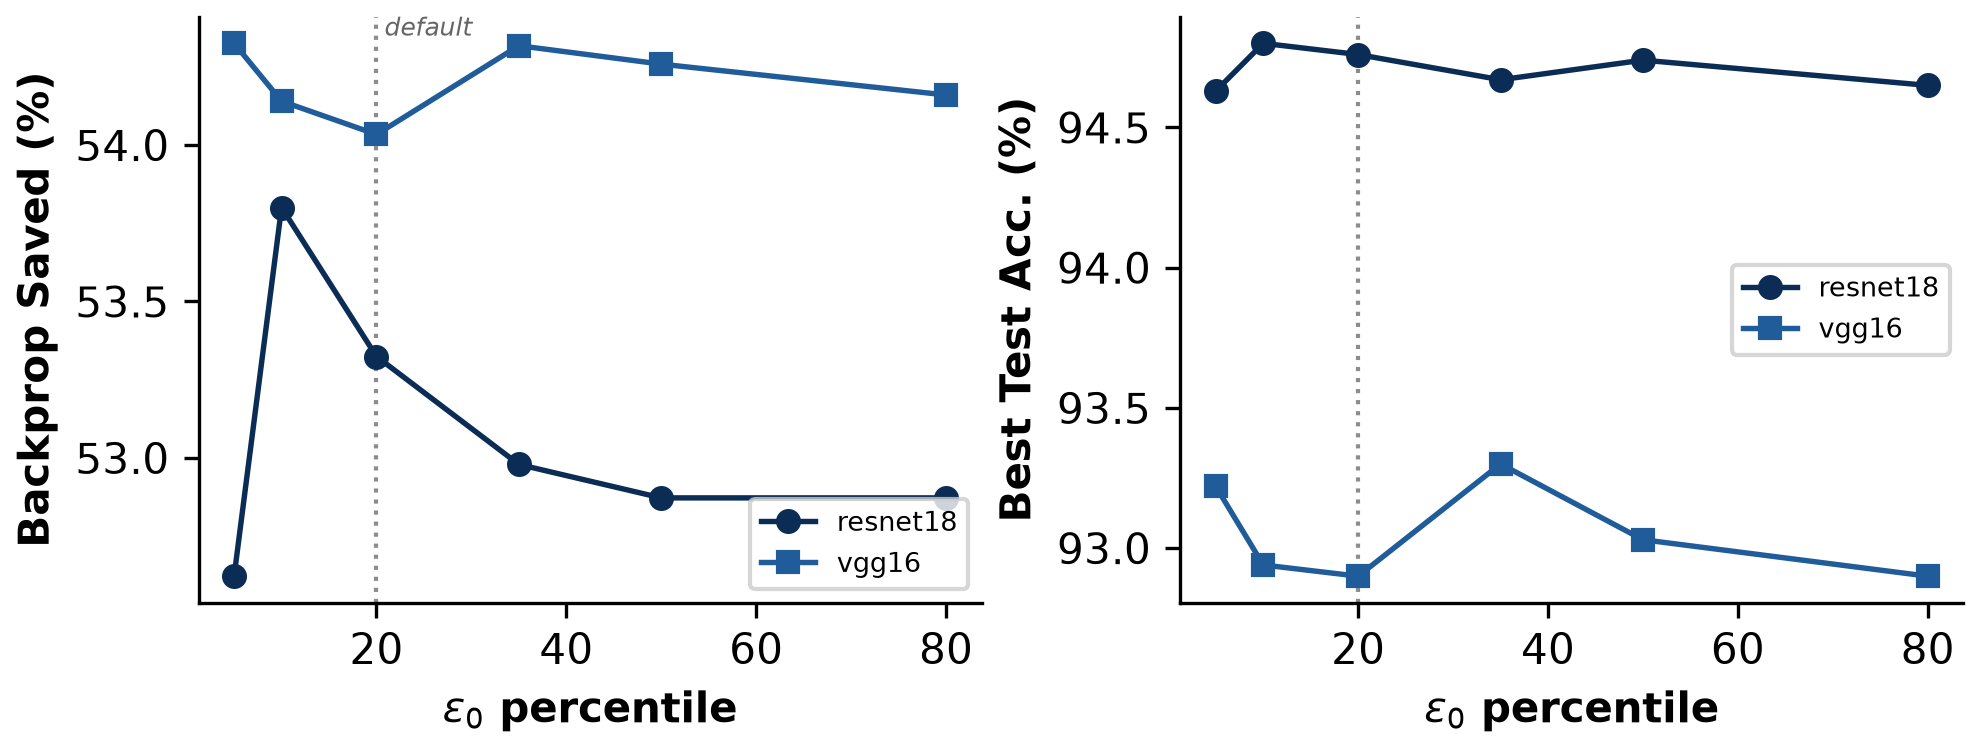
\includegraphics[width=0.85\textwidth]{figures/fig5_sensitivity.png}
\caption{Backprop saved (left) and best test accuracy (right) vs.\ gradient-norm-floor percentile, ResNet-18 and VGG-16, CIFAR-10, seed 0. Dotted line: this paper's fixed default (20th percentile, \cref{sec:selfcalib-scope}).}
\label{fig:sensitivity}
\end{figure*}

\Cref{fig:sensitivity} shows both curves are essentially flat across a 16$\times$ range of the percentile. On ResNet-18, savings vary by only $1.18$ points across the sweep ($52.6\%$ at the 5th percentile to $53.8\%$ at the 10th) and accuracy by $0.17$ points ($94.63$--$94.80\%$); on VGG-16 the range is tighter still: $0.30$ points of savings ($54.03$--$54.33\%$) and $0.40$ points of accuracy ($92.90$--$93.30\%$). Neither curve is monotonic in the percentile, which is itself informative: there is no directional trend to correct for by tuning further, just noise-level fluctuation around a stable operating point. At the paper's chosen 20th percentile, both architectures land within this same narrow band (ResNet-18: $94.76\%$/$53.32\%$; VGG-16: $92.90\%$/$54.03\%$) rather than at either extreme, so the specific choice of 20 is not doing hidden work that a different percentile would undo. The gap between architectures (VGG-16 saving roughly $0.7$--$1.7$ points more than ResNet-18 at any fixed percentile, at $\sim\!1.5$--$1.9$ points lower accuracy) is larger than the gap the percentile choice induces within either architecture, which is consistent with \cref{sec:selfcalib-scope}'s framing: the percentile is a fixed, low-sensitivity policy input, not a hyperparameter that needs per-architecture retuning within this range. This does not resolve \cref{rem:open} (the sweep is evidence the current fixed value is not fragile, not evidence that a derived value would not be preferable in principle), and we leave deriving it as future work (\cref{sec:limitations}).

\subsection{Component Ablation: Which Mechanism Drives the Gains?}
\label{sec:ablation}

TG-IES differs from IES (literal) in two calibrated quantities: the threshold $\delta$ (\cref{cor:threshold}) and the patience $K^*$ (\cref{cor:kstar}). \Cref{tab:ablation} holds one fixed at IES (literal)'s value while calibrating the other, isolating each mechanism's contribution (primary setting, seed 0; the normalization \cref{eq:activegrad} is unchanged across all four rows, since \cref{sec:practical} already established it is numerically identical to mean normalization whenever the active set exceeds one minibatch, which holds throughout every run in this paper, so normalization is not a third ablatable axis here).

\begin{table}[h]
\caption{Component ablation, primary setting, seed 0. Starred values are calibrated (reached by epoch 200); unstarred are held fixed at IES (literal)'s values. Not color-coded like the other tables: these four rows are deliberately-crippled variants of TG-IES itself, not competing methods, so ``highest number'' is not the same as ``better'' here (\cref{sec:ablation}).}
\label{tab:ablation}
\vskip 0.1in
\begin{center}
\begin{small}
\begin{tabular}{lcccc}
\toprule
Setting & Acc.\ (\%) & Saved (\%) & $\delta$ & $K^*$ \\
\midrule
Neither & 94.92 & 48.59 & 0.001 & 1 \\
$\delta$ only & 94.68 & \textbf{66.62} & 0.0077* & 1 \\
$K^*$ only & 95.04 & 3.41 & 0.001 & 15* \\
Both & 94.61 & 53.48 & 0.0160* & 15* \\
\bottomrule
\end{tabular}
\end{small}
\end{center}
\vskip -0.1in
\end{table}

Two findings, neither of which we expected going in. First, \emph{calibrating $\delta$ alone, with no patience at all ($K^*{=}1$), saves more than full TG-IES} ($66.6\%$ vs.\ $53.5\%$) at comparable accuracy. Essentially all of TG-IES's savings advantage over IES (literal) traces to the threshold calibration, not the patience calibration. Second, \emph{calibrating $K^*$ alone, against the fixed strict threshold $\delta{=}0.001$, collapses savings to $3.4\%$} ($1{,}775$ of $50{,}000$ instances ever excluded). This is the paper's controlled demonstration of the \cref{rem:open} gap: an earlier version of this paper additionally pointed to an uncontrolled architecture comparison (VGG-16) as a second instance of the same collapse; \cref{sec:results} now reports that result was a reproducibility artifact rather than a real effect, so this ablation carries that empirical claim on its own. The mechanism is visible directly in the calibration: $K^*$ saturates at its ceiling ($15$, the maximum allowed) because the fixed threshold is strict enough that few instances hold $|\Delta^2 L_i|<\delta$ for even a handful of epochs in a row, let alone $15$ consecutive ones under ordinary SGD noise: the patience counter keeps getting reset before it accumulates. This is a second, controlled demonstration of exactly the failure mode \cref{rem:open} identifies as an open problem: $\delta$ and $K^*$ are calibrated independently, and a $K^*$ calibrated without a compatibly-calibrated $\delta$ (or vice versa) can silently fail even though each calibration is individually correct with respect to its own corollary. Full TG-IES lands between these two extremes ($53.5\%$) precisely because it calibrates both together, but \cref{tab:ablation} shows this joint calibration is \emph{not} simply "the best of both": it forfeits some of the raw savings the $\delta$-only setting gets for free, in exchange for the derived, non-arbitrary patience that gives \cref{thm:safe} something to certify: $\delta$-only's $K^*{=}1$ excludes an instance after a single clean epoch with no stability argument behind it at all.

\subsection{K\texorpdfstring{$^*$}{*}-Sweep and Trajectory-Divergence Instrumentation}
\label{sec:kstartraj}

\Cref{rem:shared-traj} names the paper's central open theoretical question: \cref{thm:safe} certifies only the instantaneous perturbation of a single removal decision on a \emph{shared reference trajectory}, not how far Algorithm~\ref{alg:tgies}'s actual, multi-removal trajectory drifts from the full-data one it is idealized against, over the compounding effect of hundreds of epochs and thousands of removal decisions. We do not attempt a proof of a multi-step bound here (\cref{sec:limitations} still lists that as future work), but we can and do instrument the question directly: does the real, compounding divergence stay bounded in practice, and does it move with $K^*$ the way \cref{thm:safe}'s per-step bound (which scales linearly in $K$) predicts it should?

This is a different experiment from \cref{sec:ablation}'s ``$K^*$ only'' row, which fixes $\delta$ at IES (literal)'s strict constant and lets $K^*$ collapse to its ceiling; here $\delta$ is always self-calibrated (\cref{cor:threshold}) as in ordinary TG-IES, and only the patience is held fixed at $K^*\in\{1,2,4,8,15,30\}$ (\texttt{-{}-tgies\_fix\_kstar}), isolating $K^*$'s own effect on an otherwise-normal run. Primary cell, 3 seeds per $K^*$. We additionally instrument every run (this sweep and a matched, freshly re-run 3-seed baseline) with a full-parameter snapshot every 20 epochs, and log $\|\theta^{(t)}_{\mathrm{TG\text{-}IES}} - \theta^{(t)}_{\mathrm{baseline}}\|$ against the same-seed baseline's snapshot at the matching epoch -- a direct, empirical stand-in for the quantity \cref{rem:shared-traj} says the theory does not yet bound.

\begin{table}[h]
\caption{$K^*$-sweep, primary cell, mean $\pm$ std over seeds $\{0,1,2\}$, $\delta$ self-calibrated throughout. Matched-batch baseline (same instrumentation run): $95.08\pm0.14\%$ acc.}
\label{tab:kstarsweep}
\vskip 0.1in
\begin{center}
\begin{small}
\begin{tabular}{ccc}
\toprule
$K^*$ (fixed) & Acc.\ (\%) & Saved (\%) \\
\midrule
1  & $94.55\pm0.16$ & $\mathbf{66.98\pm0.62}$ \\
2  & $94.56\pm0.08$ & $65.75\pm0.27$ \\
4  & $94.62\pm0.10$ & $63.24\pm0.44$ \\
8  & $94.80\pm0.09$ & $58.85\pm0.57$ \\
15 & $94.80\pm0.09$ & $53.38\pm0.58$ \\
30 & $\mathbf{94.87\pm0.09}$ & $44.13\pm0.40$ \\
\bottomrule
\end{tabular}
\end{small}
\end{center}
\vskip -0.1in
\end{table}

\textbf{The accuracy/savings trade-off is smooth and monotonic in $K^*$, not a cliff.} \Cref{tab:kstarsweep} shows savings falling steadily from $67.0\%$ at $K^*{=}1$ to $44.1\%$ at $K^*{=}30$ while accuracy rises from $94.55\%$ to $94.87\%$, closing roughly two-thirds of the gap to the matched baseline's $95.08\%$. $K^*{=}15$, the value every self-calibrated TG-IES run in this paper actually lands on (\cref{sec:practical}'s rounding-direction remark), sits in the middle of this frontier rather than at either extreme: more patience is uniformly safer and less patience is uniformly cheaper, exactly the direction \cref{thm:safe}'s bound predicts, with no non-monotonic surprises across the sixfold range tested.

\begin{figure}[t]
\centering
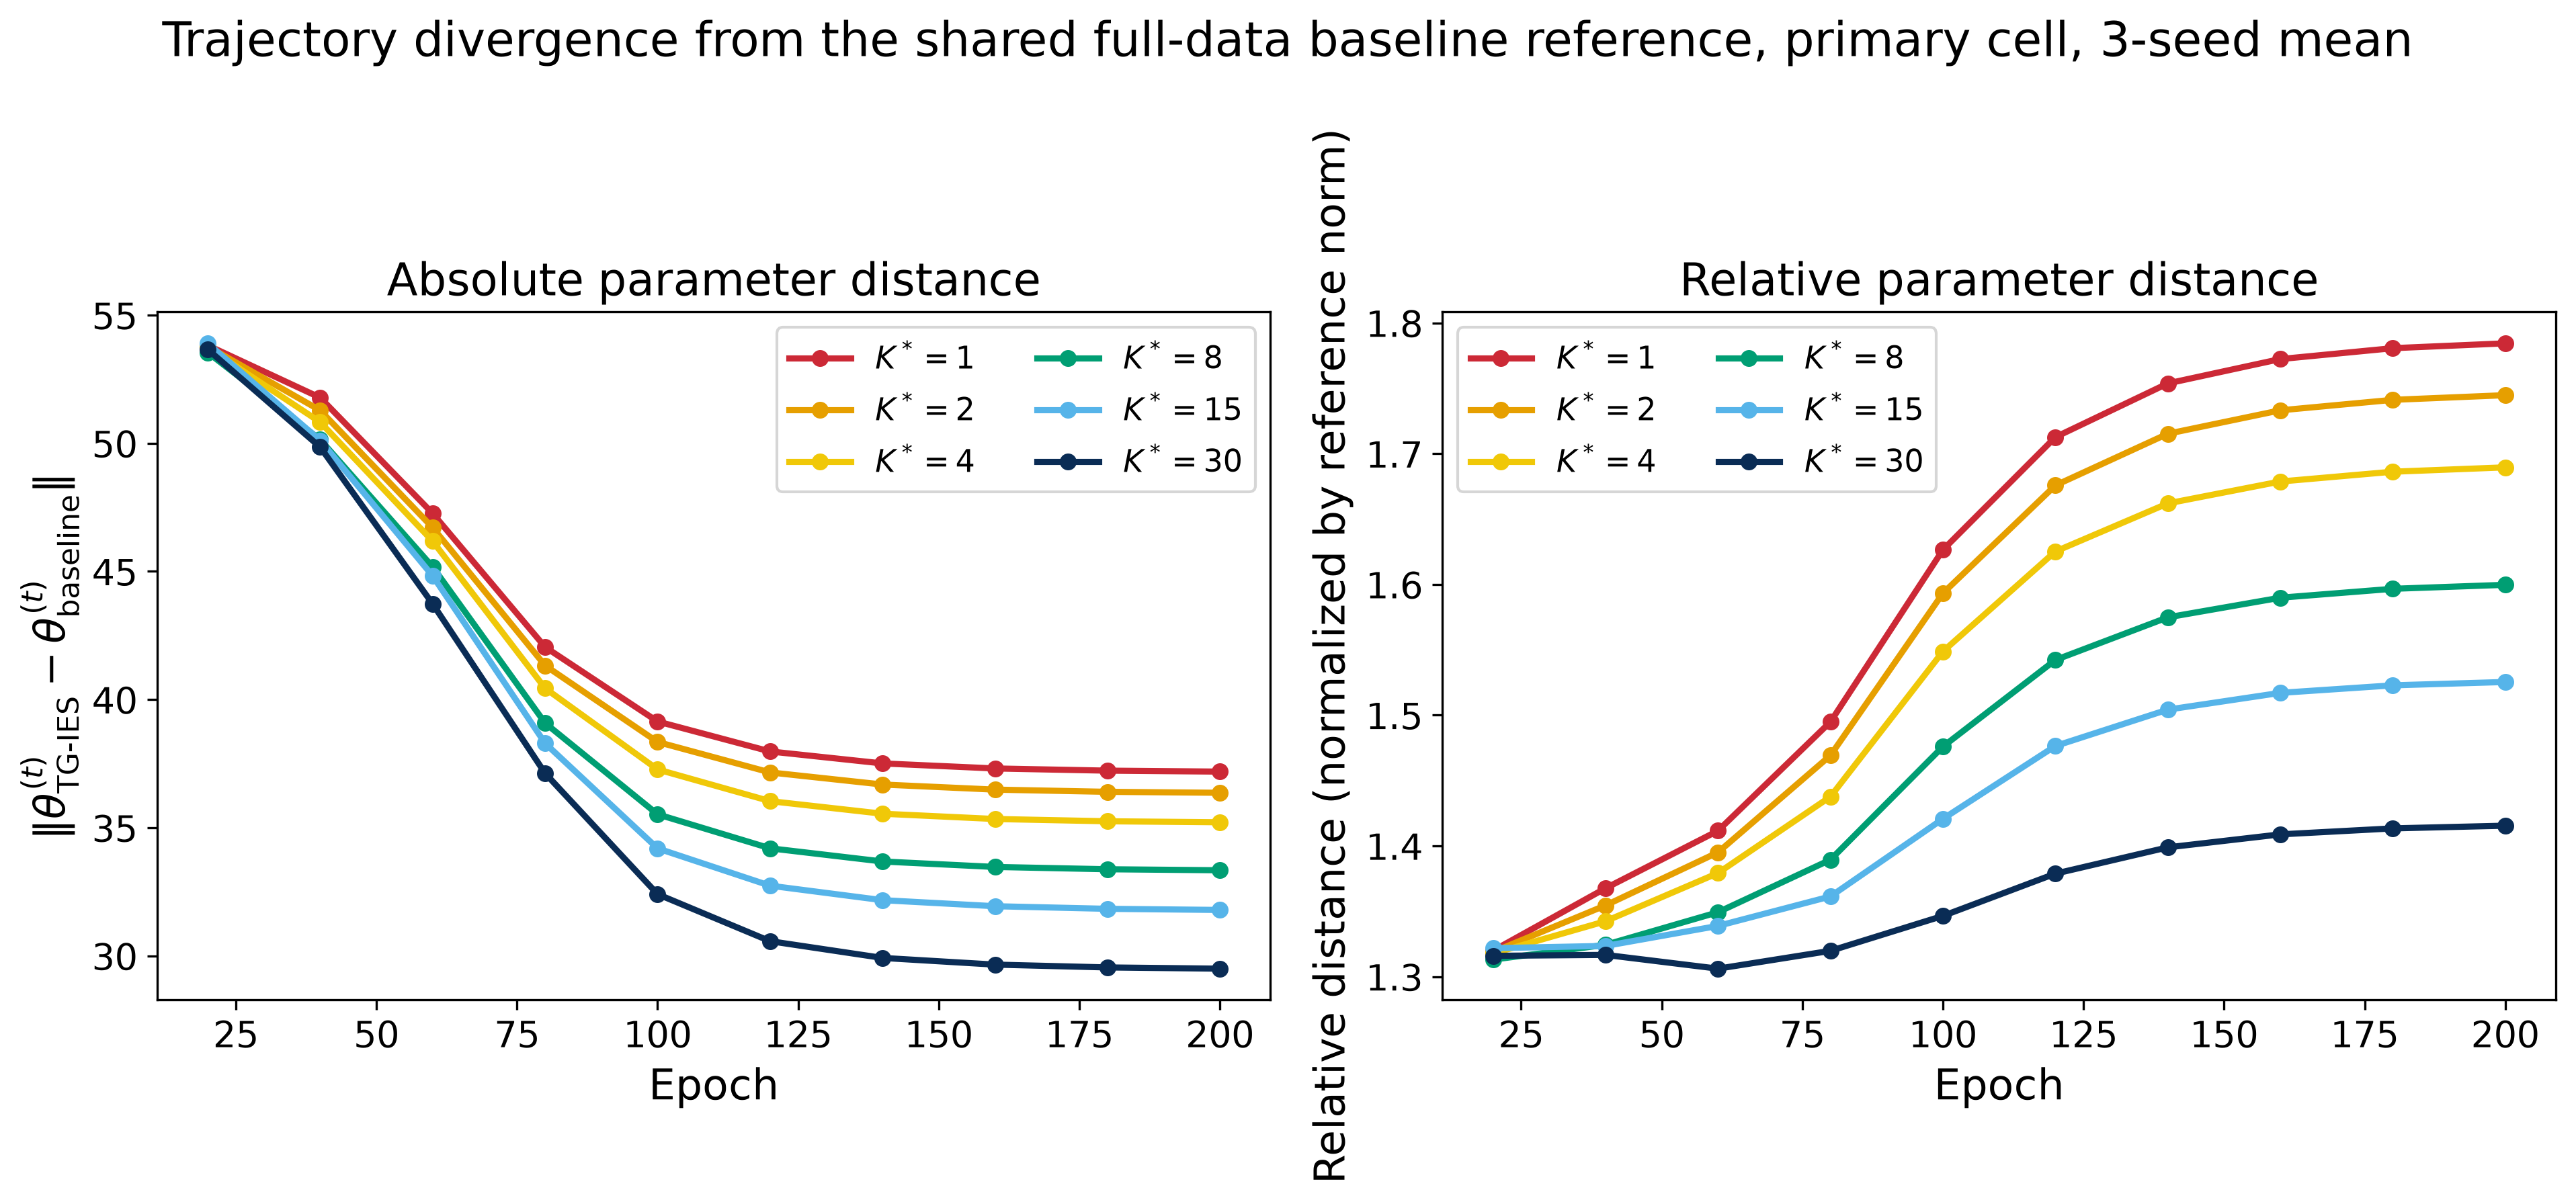
\includegraphics[width=\columnwidth]{figures/fig_kstar_trajectory.png}
\caption{Parameter-space distance between TG-IES's actual trajectory and the shared-seed baseline reference, vs.\ epoch, one curve per fixed $K^*$, 3-seed mean. Left: absolute distance $\|\theta^{(t)}_{\mathrm{TG\text{-}IES}}-\theta^{(t)}_{\mathrm{baseline}}\|$. Right: the same distance normalized by the baseline's own parameter norm at that epoch.}
\label{fig:kstartraj}
\end{figure}

\textbf{The actual trajectory does not diverge without bound, and the $K^*$-ordering matches the theory's direction.} \Cref{fig:kstartraj} (left) shows the striking part of this result: \emph{absolute} parameter distance from the baseline reference \emph{decreases} over training for every $K^*$ tested, from $\approx\!54$ at epoch $20$ down to $29$--$37$ by epoch $200$, then visibly plateaus over the last third of training -- the opposite of the unbounded-compounding-drift failure mode \cref{rem:shared-traj} leaves open as a logical possibility. At every one of the 10 snapshot epochs, the ordering across $K^*$ values is exactly what \cref{thm:safe}'s per-step bound predicts (smaller $K^*$, i.e.\ less patience before exclusion, more removal decisions, larger divergence): $K^*{=}1$'s curve sits above every other curve throughout, $K^*{=}30$'s sits below every other curve throughout, with no crossings. This is not an artifact of one seed or one snapshot: it holds at all 10 snapshot epochs and, since each point is itself a 3-seed mean, is not a single-run coincidence either. \Cref{fig:kstartraj} (right) shows the same distance normalized by the baseline's own parameter norm at that epoch instead \emph{rises} over training and appears to plateau at a higher value, purely because the reference norm itself shrinks faster (weight decay pulls both trajectories toward smaller-norm solutions, and the baseline's norm shrinks proportionally faster than the absolute gap between the two trajectories does): the reference norm falls from $40.7$ to $20.8$ over the same window, a $2\times$ contraction that the numerator does not match. We report both panels rather than only the more optimistic-looking one, since which normalization is the "right" one to read \cref{rem:shared-traj}'s open question through is itself not settled by this experiment.

\textbf{What this does and does not establish.} This is empirical evidence, on one architecture/dataset/schedule and $200$-epoch horizon, that Algorithm~\ref{alg:tgies}'s actual multi-removal trajectory behaves consistently with -- and does not obviously violate -- the direction \cref{thm:safe}'s single-window certificate would predict if it extended to the full run, and does not exhibit the specific worst-case failure (unbounded compounding drift) that \cref{rem:shared-traj} could not rule out theoretically. It is not a proof, does not generalize past this setting without further evidence, and does not by itself close the gap: a genuine multi-step bound would still need to establish this behavior analytically, under stated assumptions, for it to be a certificate rather than an observation on this paper's own runs. We update \cref{sec:limitations}'s framing of this gap accordingly -- from "untested" to "empirically consistent with, formally still open" -- rather than claim more than the data supports.

\section{Conclusion}
\label{sec:conclusion}

We set out to answer whether IES's mastery criterion (the magnitude of a backward second-order loss difference, \cref{eq:mastery}) admits a theoretical grounding, and whether that grounding could replace IES's hand-tuned threshold and patience with quantities calibrated from the training run itself. \Cref{sec:selfcalib-scope} is explicit about the scope of that claim: $\delta$ and $K^*$ themselves are derived, not hand-tuned, but deriving them still costs a small number of fixed policy inputs rather than zero configuration. On the theory side we established five results under explicit, stated idealizations: an exact scale-cancellation identity (\cref{thm:ratio}) giving theorem-level content to IES's informal ``scale invariance''; an exact bias--variance decomposition and an explicit SNR regime (\cref{thm:bv,prop:mse}) explaining why second-order differencing specifically, not first or third; a corrected decomposition (\cref{thm:curvature}) showing the signal is asymptotically dominated by an $O(\eta)$ gradient-drift term rather than pure curvature, as a naive reading would assume, though \cref{sec:lrmechanism}'s direct instrumentation of $D_i^{(t)}$ finds this asymptotic ordering does not translate into empirical dominance at this paper's actual step sizes; a parameter-stability bound (\cref{thm:safe}) -- a conditional, local stability certificate, not a guarantee over TG-IES's actual multi-removal training trajectory (\cref{rem:shared-traj}) -- yielding closed-form $\delta$ and $K^*$ (\cref{cor:threshold,cor:kstar}), instantiated as TG-IES (\cref{alg:tgies}); and, under two further idealizations beyond the first four results, a direct bridge from the mastery signal to a gradient-norm bound (\cref{thm:bridge,cor:bridgeprob}), closing most of what \cref{rem:open} originally left as an unresolved link.

On the empirical side, the picture that emerges across the primary CIFAR-10 matrix, the now seed-averaged CIFAR-100 cell, and the component ablation (\cref{sec:ablation}) is more precise than ``TG-IES works,'' and we think the more precise version is the more useful conclusion. It is specifically the calibrated threshold $\delta$ that carries essentially all of TG-IES's savings advantage over IES (literal); the calibrated patience $K^*$ contributes the derived stability certificate of \cref{thm:safe} rather than additional savings, and, calibrated against a mismatched $\delta$, can collapse savings to near zero (\cref{sec:ablation}). So the claim this paper supports is not ``both calibrated quantities help equally,'' but ``the threshold calibration does the practical work, and the patience calibration is what turns removal into a certified rather than an arbitrary decision, provided the idealizations \cref{sec:bridge} states hold closely enough.'' We view stating exactly where those idealizations can fail, in a controlled ablation, as a more useful contribution than a single aggregate accuracy-vs-compute number would have been. We note that \cref{sec:bridge}'s idealizations and the ablation's mismatched-$\delta$/$K^*$ collapse are two distinct manifestations of the same underlying gap rather than one explaining the other: \cref{rem:bridge-scope}'s caveats bound when the noiseless mastery signal fails to certify a small gradient norm at all, while the ablation shows a separate, calibration-level failure mode (patience derived for one $\delta$ applied against an incompatible one); connecting the two mechanistically is exactly the kind of gap \cref{sec:limitations} still lists as open. A reproducibility audit of this version also corrected a VGG-16 result an earlier version had read as a second instance of this same gap (\cref{sec:results}); we view catching and reporting that correction as part of the rigor this claim needs, not a footnote to it.

\section{Limitations}
\label{sec:limitations}

\textbf{Idealized assumptions, and the central open theoretical question.} \Cref{ass:geometric,ass:noise,ass:dispersion,ass:smoothi} are stated idealizations (local geometric decay, time-independent noise, small rate dispersion, per-instance smoothness). Of these, the most consequential is the one \cref{rem:shared-traj} names directly: \cref{thm:safe} is a \emph{conditional, local} stability certificate for a single removal's instantaneous perturbation, evaluated on a shared reference trajectory, not a guarantee that Algorithm~\ref{alg:tgies}'s actual training trajectory (built from many such removals, each changing the trajectory every later removal decision is then evaluated against) stays close to the full-data trajectory over an entire run. We consider this the paper's most important open theoretical question, ahead of any other idealization listed here, because it is the one a reader could otherwise mistake \cref{thm:safe,cor:kstar} as already answering; \cref{sec:kstartraj} now instruments the actual quantity directly (finding it plateaus rather than diverging, over $200$ epochs on the primary cell), \cref{app:multistep} reports a first attempted formal bound (correct but exponentially loose, \cref{prop:multistep}, with the missing ingredient for a tighter one named in \cref{rem:contraction-direction}), and future-work item (5) below states precisely what still remains.

\textbf{A partly closed open problem.} \Cref{rem:open} originally stated that the noise-based mastery check ($\hat S_i<\delta$) and the gradient-norm safety condition ($\|g_i^{(t)}\|<\varepsilon$) that justifies \cref{thm:safe} were not formally linked. \Cref{sec:bridge} closes most of this link (\cref{thm:bridge,cor:bridgeprob}), but only under two further idealizations beyond \cref{ass:geometric} (per-instance smoothness, \cref{ass:smoothi}; a shared interpolating solution, \cref{rem:smoothi-why}) and with two remaining caveats \cref{rem:bridge-scope} states precisely: the bound is only informative for instances with $r_i$ bounded away from $1$, and the proved probabilistic statement is a joint, not conditional, probability bound. To the extent these do not hold, $\delta$ and $K^*$ should still be treated as calibrated independently. \Cref{sec:ablation} demonstrates the resulting failure mode directly and controllably (calibrating $K^*$ against a mismatched fixed $\delta$ collapses savings to $3.4\%$); an earlier version of this paper additionally read a VGG-16 result as a second, architecture-level instance of the same gap, which \cref{sec:results} reports was in fact a reproducibility artifact, now corrected.

\textbf{Empirical scope.} Two datasets (CIFAR-10, and a now seed-averaged second dataset, CIFAR-100, \cref{sec:cifar100}); four architectures on CIFAR-10 (ResNet-18, VGG-16, DenseNet-121, \cref{sec:densenet}, and a fourth architecture family beyond convolutions entirely, ViT-Tiny, \cref{sec:vit}, also run on CIFAR-100); three seeds on the CIFAR-10 primary cell, both secondary cells (ResNet-18/exponential, ResNet-18/fixed, VGG-16/exponential), the Adam cell (\cref{sec:adam}), the CIFAR-100 cell, the DenseNet-121 cell (backfilled from single-seed after this paper's first version, the same as CIFAR-100 and Adam), and both ViT-Tiny cells (3-seed from the start). Every three-seed cell in this paper, DenseNet-121 and ViT-Tiny included, is quantified directly by the paired statistical analysis in \cref{app:stats}. The two cells (fixed-LR, VGG-16) affected by the stale recalibration-timing configuration described in \cref{sec:results} were specifically re-audited for that issue before being reported as seed-averaged; CIFAR-100's seed-0 run was checked against the same criterion (delta recalibrating once, at epoch 30, not epoch-over-epoch) and was not affected, so its backfilled seeds 1--2 could be added directly without a corresponding correction.

\textbf{Recalibration schedule is empirical, not derived.} \Cref{sec:practical} reports that one-time (rather than repeating) recalibration was chosen because repeating recalibration was found empirically to strangle savings; this specific engineering choice does not follow from \cref{cor:threshold,cor:kstar} themselves.

\textbf{Metric convention.} Reported accuracy is best-over-200-epochs, matching \citet{yuan2025instance}'s convention. We checked this against final-epoch accuracy across all 20 runs: the gap averages $0.38$ points and never exceeds $0.81$ points, and is similar across methods (mean per-method gap $0.32$--$0.45$ points, with baseline, not TG-IES, showing the largest mean gap), so this convention does not favor any one method or change the accuracy--compute trade-off reported in \cref{sec:results}, though we still report best-over-training rather than final-epoch throughout, as \citet{yuan2025instance} do.

\textbf{Future work.} Concrete gaps we have not closed, named specifically rather than left implicit: (1) \emph{Scale.} All experiments are on CIFAR-scale images; larger-scale benchmarks such as TinyImageNet or ImageNet-100 would test whether the calibration (in particular the gradient-norm-floor proxy behind $K^*$) transfers to higher-resolution inputs and larger class counts, and we have not run them. (2) \emph{Architecture family, now partly closed.} An earlier version of this paper flagged a transformer as untried, since a poorly-tuned ViT baseline would confound the comparison rather than inform it; \cref{sec:vit} now adds one (a CIFAR-native ViT-Tiny, validated to train to reasonable accuracy before comparison), and the calibration does transfer -- the savings advantage holds and grows with task difficulty using the same four fixed constants as every convolutional cell -- but at materially smaller absolute savings and a small accuracy cost not seen on ResNet-18, VGG-16, or DenseNet-121. What remains open: a larger transformer (ViT-Small, DeiT-Tiny) or one at a resolution where patch-16 tokenization is meaningful, both deferred alongside item (1)'s scale question rather than attempted here; and whether raising \cref{sec:vit}'s \texttt{-{}-max\_kstar} ceiling (pinned at every ViT run in this paper) changes the picture, which we flag but did not test. (3) \emph{Optimizer/schedule sensitivity.} \Cref{sec:results,sec:adam} show TG-IES trailing simpler IES variants specifically on the two settings without the exponential LR schedule (fixed-LR SGD, Adam); \cref{sec:lrmechanism} proposes a candidate mechanism (the drift term of \cref{thm:curvature} losing its shrinking prefactor under non-decaying $\eta$) and now also instruments $D_i^{(t)}$ directly, which complicates rather than confirms the mechanism (\cref{fig:driftvalidation}: the drift term correlates only weakly with the observed signal and does not dominate the curvature-plus-remainder term at this network's actual step sizes). The controlled ablation calibrating $\delta,K^*$ under a matched noise/gradient-norm profile across schedules remains unrun. A related, now partly closed gap: \cref{fig:driftvalidation} originally used only $\langle g_i^{(t)},g^{(t)}\rangle$ (a scalar dot product, saved to keep memory/disk small), not $\|g_i^{(t)}\|$ itself, so \cref{cor:bridgeprob}'s calibration-bound check could not be tested directly. We extended \texttt{drift\_term\_run.py} to also save $\|g_i^{(t)}\|$ and reran all three schedules; \cref{sec:bridge}'s empirical check now confirms the qualitative relationship \cref{thm:bridge} predicts ($\|g_i^{(t)}\|$ correlates with $\sqrt{|\Delta^2L_i^{(t)}|}$ at $r{\approx}0.5$; mastery-check-passing instances have $30$--$33\times$ smaller gradient norms) across all three schedules. What remains open is only the \emph{exact} bound $\varepsilon_i(\delta)$, which needs per-instance $r_i,\Lambda_i$ this paper does not estimate; the qualitative direction is no longer untested. (4) \emph{RHO-LOSS and RL-style dynamic pruning.} \Cref{sec:newbaselines} adds InfoBatch, BLS-InfoBatch, and AlignPrune, but not RHO-LOSS \citep{mindermann2022prioritized} (which needs a holdout model) or DPPO-style methods \citep{zhu2026dppo} (a different, RL problem setting); both are natural next comparisons. (5) \emph{A multi-step trajectory-divergence bound, now empirically probed but not yet proved.} \Cref{thm:safe} certifies only the instantaneous, single-window perturbation of one removal decision on a shared reference trajectory (\cref{rem:shared-traj}); it does not bound how far Algorithm~\ref{alg:tgies}'s actual trajectory, shaped by every removal decision made so far, drifts from the full-data trajectory over hundreds of epochs of compounding removals. \Cref{sec:kstartraj} adds direct instrumentation of exactly this quantity, $\|\theta_t^{\mathrm{full}}-\theta_t^{\mathrm{TG\text{-}IES}}\|$ against a shared-seed baseline reference, across a sixfold range of $K^*$: on the primary cell, over $200$ epochs, absolute divergence plateaus rather than growing without bound, and the $K^*$-ordering matches the direction \cref{thm:safe}'s bound predicts at every snapshot epoch. This is evidence against the specific worst-case failure mode (unbounded compounding drift) that was previously untested, on one architecture/dataset/schedule -- it is not evidence that such a bound holds in general, and does not reduce the need for one. We now report a first attempt at exactly this (\cref{app:multistep}): under \cref{ass:smooth}'s $\beta$-smoothness plus \cref{thm:safe}'s own gradient-floor hypothesis extended to hold along the algorithm's real trajectory, a discrete Gronwall-style argument (\cref{prop:multistep}) does bound $\|\theta_t^{\mathrm{full}}-\theta_t^{\mathrm{TG\text{-}IES}}\|$ as a function of $t,\eta,\beta,\varepsilon_i,N$ -- but the bound grows exponentially in $t$ and is vacuous over a full $\sim\!200$-epoch run, explaining mechanistically why a Lipschitz-only argument cannot give a useful multi-step certificate, rather than merely asserting the gap. \Cref{rem:contraction-direction} identifies what would fix this: an additional local strong-convexity or PL condition along the trajectory would turn the same recursion into a contraction with a bounded, $t$-independent limit, qualitatively matching \cref{sec:kstartraj}'s empirical plateau -- but we do not derive that stronger result here, since it needs an assumption we have not verified for the architectures in this paper. Closing this fully still needs that derivation, done rigorously; we view it as the single most important theoretical gap remaining in this paper, ahead of items (1)--(4), now with a documented first attempt and a concrete, named next step rather than an unattempted one.

\section*{Impact Statement}
This paper presents work whose goal is to advance the field of Machine Learning, specifically compute-efficient training. There are many potential societal consequences of our work, none which we feel must be specifically highlighted here.

\bibliography{references}
\bibliographystyle{icml2025}

\newpage
\appendix
\onecolumn

\section{Full Proofs}
\label{app:proofs}

\begin{proof}[Proof of \cref{lem:geomdiff}]
\emph{Proof idea: this is bookkeeping, not a deep argument.} Differencing a geometric sequence once multiplies it by $(r_i-1)$ and shifts the exponent down by one; doing this $N$ times just multiplies by $(r_i-1)^N$ in total, which induction makes precise below.

Induction on $N$.

\emph{Base case} ($N=0$): $\Delta^0(L_i^{(t)}-L^*) = c_i r_i^t$.

\emph{Inductive step.} Assume $\Delta^{N-1}(L_i^{(t)}-L^*) = c_i r_i^{t-(N-1)}(r_i-1)^{N-1}$. Then
\begin{align*}
\Delta^N(L_i^{(t)}-L^*) &= \Delta^{N-1}(L_i^{(t)}-L^*) - \Delta^{N-1}(L_i^{(t-1)}-L^*) \\
&= c_i\, r_i^{t-N+1}(r_i-1)^{N-1} - c_i\, r_i^{t-N}(r_i-1)^{N-1} \\
&= c_i(r_i-1)^{N-1}\big(r_i^{t-N+1}-r_i^{t-N}\big) \\
&= c_i\,r_i^{t-N}(r_i-1)^N,
\end{align*}
which is the claim for $N$.
\end{proof}

\begin{proof}[Proof of \cref{thm:ratio}]
\emph{Proof idea:} \cref{lem:geomdiff} already gives a closed form for both the $N$th and $(N-1)$th differences; dividing one by the other is pure algebra, and everything that depends on the instance's identity ($c_i$, and most of the powers of $r_i$) cancels, leaving only a simple ratio in $r_i$.

By \cref{lem:geomdiff},
\begin{align*}
\Delta^N(L_i^{(t)}-L^*) &= c_i\, r_i^{t-N}(r_i-1)^N, \\
\Delta^{N-1}(L_i^{(t)}-L^*) &= c_i\, r_i^{t-N+1}(r_i-1)^{N-1}.
\end{align*}
Dividing the first by the second,
\begin{align*}
\frac{\Delta^N(L_i^{(t)}-L^*)}{\Delta^{N-1}(L_i^{(t)}-L^*)}
&= \frac{c_i\, r_i^{t-N}(r_i-1)^N}{c_i\, r_i^{t-N+1}(r_i-1)^{N-1}} \\
&= \frac{r_i^{t-N}}{r_i^{t-N+1}}\cdot(r_i-1) \\
&= r_i^{-1}(r_i-1) \;=\; \frac{r_i-1}{r_i},
\end{align*}
where $c_i$ cancels since it appears in both numerator and denominator. The denominator $c_i r_i^{t-(N-1)}(r_i-1)^{N-1}$ is nonzero whenever $c_i>0$, $r_i\in(0,1)$, and $N\ge1$, all guaranteed by \cref{ass:geometric}.
\end{proof}

\begin{proof}[Proof of \cref{prop:cv}]
\emph{Proof idea, before the five formal steps below:} treat every instance's rate $r_i$ as the common rate $\bar r$ plus a small deviation $\epsilon_i$ (bounded by $\delta_r$, \cref{ass:dispersion}). Steps 1--3 use a first-order (mean value theorem) argument to show that this small deviation moves both the mean and the variance of $X(N)$ by at most $O(\delta_r)$. Step 4 notes that $\CV$ is a smooth function of (mean, standard deviation), so a small change in each of those inputs produces only a small change in $\CV$ itself (a Lipschitz argument). Step 5 just applies this once for $N=1$ and once for $N=2$ and adds the two small errors together (triangle inequality) to bound their difference.

\emph{Step 1 (pointwise perturbation).} Let $f_1(r)=r^{t-1}(1-r)$ and $f_2(r)=r^{t-2}(1-r)^2$ on $[r_{\min},r_{\max}]=[\bar r-\delta_r,\bar r+\delta_r]\subset(0,1)$; both are smooth there, so
\[
L_N := \sup_{r\in[r_{\min},r_{\max}]}|f_N'(r)| < \infty.
\]
Write $r_i=\bar r+\epsilon_i$ with $|\epsilon_i|\le\delta_r$, and set $\Delta_i^{(N)} := f_N(r_i)-f_N(\bar r)$. The mean value theorem gives
\[
|\Delta_i^{(N)}| \le L_N\delta_r.
\]
Defining $Y_i^{(N)} := c_i f_N(\bar r)$ and $E_i^{(N)} := c_i\Delta_i^{(N)}$,
\[
X_i(N) = Y_i^{(N)} + E_i^{(N)}, \qquad |E_i^{(N)}| \le c_{\max}L_N\delta_r.
\]

\emph{Step 2 (mean perturbation).}
\[
|\mathbb E[X(N)]-\mathbb E[Y(N)]| \le c_{\max}L_N\delta_r,
\]
and consequently $\mathbb E[X(N)] \ge c_{\min}f_N(\bar r) - c_{\max}L_N\delta_r > 0$ whenever $\delta_r < c_{\min}f_N(\bar r)/(c_{\max}L_N)$.

\emph{Step 3 (variance perturbation).} Since $\Var(X(N)) = \mathbb E[X(N)^2] - \mathbb E[X(N)]^2$, and
\[
X_i(N)^2 - Y_i(N)^2 = E_i^{(N)}\big(2Y_i^{(N)} + E_i^{(N)}\big),
\]
with $|E_i^{(N)}|\le c_{\max}L_N\delta_r$ and $|Y_i^{(N)}|\le c_{\max}f_N(\bar r+\delta_r)$, this difference is $O(\delta_r)$ uniformly. Combined with Step 2's bound on the means,
\[
|\Var(X(N)) - \Var(Y(N))| \le (A_N+B_N)\delta_r
\]
for finite constants $A_N,B_N$, and hence, absorbing constants,
\[
\big|\sqrt{\Var(X(N))} - \sqrt{\Var(Y(N))}\big| \le D_N\delta_r
\]
for a finite constant $D_N$.

\emph{Step 4 (Lipschitz bound on CV).} The map $\phi(\mu,s)=s/\mu$ is $C^1$ on $\mu>0$, with bounded gradient $\Lambda_N$ on the compact region containing both $(\mathbb E[X(N)],\sqrt{\Var(X(N))})$ and $(\mathbb E[Y(N)],\sqrt{\Var(Y(N))})$ for small $\delta_r$. Combining Steps 2--3 with $\phi$'s Lipschitz property,
\[
|\CV(X(N)) - \CV(Y(N))| \le \Lambda_N(c_{\max}L_N + D_N)\,\delta_r.
\]

\emph{Step 5 (combining orders).} Since $Y_i^{(N)} = c_i f_N(\bar r)$ is $c_i$ scaled by a constant,
\[
\CV(Y(N)) = \frac{\sqrt{\Var(c)}}{\mathbb E[c]}
\]
is identical for $N=1$ and $N=2$: the $f_N(\bar r)$ factor cancels in the ratio. Applying Step 4 to both orders and the triangle inequality,
\[
|\CV(X(1)) - \CV(X(2))| \le \big(\Lambda_1(c_{\max}L_1+D_1) + \Lambda_2(c_{\max}L_2+D_2)\big)\delta_r,
\]
which is the claim with $C := \max_{N\in\{1,2\}}\Lambda_N(c_{\max}L_N+D_N)$, made explicit in \cref{app:constants}.
\end{proof}

\begin{proof}[Proof of \cref{thm:bv}]
\emph{Proof idea:} split the noisy $N$th difference into ``signal'' (the deterministic part from \cref{lem:geomdiff}) plus ``noise'' (a specific weighted sum of the $N{+}1$ raw noise terms $\xi_{i,t},\dots,\xi_{i,t-N}$ that differencing produces). Squaring and taking expectations, the signal contributes its own square, the noise contributes its variance, and the signal-noise cross term vanishes because noise is mean-zero. The noise's variance is then just ``sum of squared differencing coefficients times $\sigma^2$,'' and those coefficients happen to be binomial coefficients, so their sum of squares is the textbook Vandermonde identity $\sum_k\binom{N}{k}^2=\binom{2N}{N}$, the source of the $\binom{2N}{N}\sigma^2$ term.

By linearity, $\Delta^N\tilde L_i^{(t)} = \Delta^N L_i^{(t)} + \Delta^N\xi_{i,t}$. Set
\[
a := \Delta^N L_i^{(t)} = c_i r_i^{t-N}(r_i-1)^N
\]
(deterministic given $\theta^{(t)}$, by \cref{lem:geomdiff}) and
\[
b := \Delta^N\xi_{i,t} = \sum_{k=0}^N(-1)^k\binom Nk\xi_{i,t-k}.
\]
Then
\[
\mathbb E\big[(\Delta^N\tilde L_i^{(t)})^2\big] = a^2 + 2a\,\mathbb E[b] + \mathbb E[b^2].
\]
By \cref{ass:noise}, $\mathbb E[\xi_{i,t-k}]=0$, so $\mathbb E[b]=0$ and the cross term vanishes. Since the $\xi_{i,t-k}$ are independent with variance $\sigma^2$,
\[
\mathbb E[b^2] = \Var(b) = \sigma^2\sum_{k=0}^N\binom Nk^2 = \sigma^2\binom{2N}N
\]
by the Vandermonde identity. Combining the last three displays gives \cref{eq:bv}.
\end{proof}

\begin{proof}[Proof of \cref{prop:mse}]
\emph{Proof idea:} \cref{thm:bv} already gives an exact formula for $\mathrm{MSE}(N,t)$; this proof just plugs in $N=1,2,3$, factors out what the three formulas share, and directly compares the results two at a time. Each comparison reduces to checking the sign of a single quantity, and both comparisons can be satisfied simultaneously (i.e., $N=2$ beats both neighbors at once) exactly on the two-sided band in \cref{eq:band}, which turns out to always contain at least one valid value whenever $r_i>\tfrac12$.

Write $\alpha_i := (1-r_i)^2/r_i^2$, so that
\[
r_i^{2(t-N)}(r_i-1)^{2N} = r_i^{2t}\big[(1-r_i)^2/r_i^2\big]^N = r_i^{2t}\alpha_i^N
\]
(using $(r_i-1)^2=(1-r_i)^2$), and hence $\mathrm{MSE}(N,t) = c_i^2 r_i^{2t}\alpha_i^N + \binom{2N}N\sigma^2$. Using $\binom21=2$, $\binom42=6$, $\binom63=20$:
\begin{align*}
\mathrm{MSE}(1,t)-\mathrm{MSE}(2,t) &= c_i^2r_i^{2t}(\alpha_i-\alpha_i^2) - 4\sigma^2 \\
&= c_i^2r_i^{2t}\alpha_i(1-\alpha_i)-4\sigma^2,
\end{align*}
giving \cref{eq:mse12}. Similarly,
\begin{align*}
\mathrm{MSE}(3,t)-\mathrm{MSE}(2,t) &= c_i^2r_i^{2t}(\alpha_i^3-\alpha_i^2) + 14\sigma^2 \\
&= 14\sigma^2 - c_i^2r_i^{2t}\alpha_i^2(1-\alpha_i),
\end{align*}
giving \cref{eq:mse23}. For $\alpha_i<1$ (i.e.\ $r_i>\tfrac12$), $(1-\alpha_i)>0$, so both conditions impose genuine (non-degenerate) two-sided bounds on $c_i^2r_i^{2t}$, combining into \cref{eq:band}. Non-emptiness: the lower bound does not exceed the upper bound iff $4\alpha_i\le14$, i.e.\ $\alpha_i\le3.5$, which holds for every $\alpha_i<1$.
\end{proof}

\begin{proof}[Proof of \cref{cor:threshold}]
\emph{Proof idea:} $\Delta^2\xi_{i,t}$ is a fixed combination $(1,-2,1)$ of three independent noise draws, so its variance is just the sum of the squared coefficients ($1+4+1=6$) times $\sigma^2$, a special case of the general variance formula from \cref{thm:bv} at $N=2$. Once that variance is known, converting it into a probability that $|\Delta^2\xi_{i,t}|$ exceeds a threshold $\delta$ is a standard step: exactly (via the Gaussian CDF $\Phi$) if the noise is Gaussian, or as a guaranteed upper bound (via the sub-Gaussian tail inequality) if it is merely sub-Gaussian.

By \cref{ass:noise} (independence),
\[
\Var(\Delta^2\xi_{i,t}) = \Var(\xi_{i,t}-2\xi_{i,t-1}+\xi_{i,t-2}) = \sigma^2\big(1^2+(-2)^2+1^2\big) = 6\sigma^2,
\]
matching \cref{thm:bv} at $N=2$, which needs only \cref{ass:noise}. The Gaussian tail approximation is standard. Under \cref{ass:subgaussian}, $\Delta^2\xi_{i,t}$ is a linear combination of independent $\sigma^2$-sub-Gaussian variables with squared coefficients summing to $6$, hence itself $6\sigma^2$-sub-Gaussian; the standard sub-Gaussian tail inequality then gives the stated bound $2\exp(-k^2/2)$.
\end{proof}

\begin{proof}[Proof of \cref{thm:curvature}]
\emph{Proof idea:} write down the standard Taylor expansion of the loss after one gradient-descent step, once centered at $t{-}1$ and once at $t{-}2$; each expansion has a linear (gradient) term, a quadratic (curvature) term, and a leftover remainder that a bounded-third-derivative assumption (\cref{ass:thirdderiv}) keeps small. The second difference $\Delta^2 L_i^{(t)}$ is literally ``the first expansion minus the second,'' so subtracting them lines up the two linear terms into the drift piece, the two quadratic terms into the curvature piece, and the two remainders into one bounded leftover term; no step here does anything beyond substitution and bookkeeping.

Let $\Delta\theta^{(s)}=\theta^{(s+1)}-\theta^{(s)}=-\eta g^{(s)}$ (full-batch). By third-order Taylor expansion with remainder (\cref{ass:thirdderiv}),
\[
L_i(\theta^{(s)}+\Delta\theta^{(s)}) = L_i(\theta^{(s)}) + \langle g_i^{(s)},\Delta\theta^{(s)}\rangle + \tfrac12\Delta\theta^{(s)\top}H_i(\theta^{(s)})\Delta\theta^{(s)} + r_{i,s},
\]
with $|r_{i,s}|\le\frac{M_3}6\|\Delta\theta^{(s)}\|^3=\frac{M_3}6\eta^3\|g^{(s)}\|^3$. Substituting $\Delta\theta^{(s)}=-\eta g^{(s)}$ and applying at $s=t-1,t-2$:
\[
L_i^{(t)} = L_i^{(t-1)} - \eta\langle g_i^{(t-1)},g^{(t-1)}\rangle + \tfrac{\eta^2}2 g^{(t-1)\top}H_i(\theta^{(t-1)})g^{(t-1)} + r_{i,t-1},
\]
\[
L_i^{(t-1)} = L_i^{(t-2)} - \eta\langle g_i^{(t-2)},g^{(t-2)}\rangle + \tfrac{\eta^2}2 g^{(t-2)\top}H_i(\theta^{(t-2)})g^{(t-2)} + r_{i,t-2}.
\]
Forming
\[
\Delta^2 L_i^{(t)} = L_i^{(t)}-2L_i^{(t-1)}+L_i^{(t-2)} = \big[L_i^{(t)}-L_i^{(t-1)}\big]-\big[L_i^{(t-1)}-L_i^{(t-2)}\big]
\]
and substituting both expansions above, the $O(\eta)$ terms combine into $\eta\big(\langle g_i^{(t-2)},g^{(t-2)}\rangle-\langle g_i^{(t-1)},g^{(t-1)}\rangle\big)$ and the $O(\eta^2)$ terms into the bracketed difference in \cref{eq:curvature}. Setting $R_{i,t}:=r_{i,t-1}-r_{i,t-2}$ and applying the triangle inequality to the two remainder bounds gives \cref{eq:curvature} with the stated remainder bound.
\end{proof}

\begin{proof}[Proof of \cref{thm:safe}]
\emph{Proof idea:} the two runs being compared use the exact same update rule, so at every step the only possible source of disagreement is whether instance $i$'s own gradient term is included. That means each single step can push the two parameter vectors apart by at most $\eta\|g_i^{(t)}\|/N$, the size of the one term that differs, scaled by the step size and the $1/N$ normalization. Adding up $K$ such small pushes (triangle inequality) bounds the total gap after $K$ steps, and a Lipschitz test loss cannot turn a small parameter gap into a large accuracy gap, which gives the second bound for free.

At each $t\in[T-K,T]$, both runs use \cref{eq:activegrad} evaluated on the same reference trajectory, so the only difference between the two update directions is the presence or absence of the term $\frac1N g_i^{(t)}$. The per-step parameter deviation is therefore bounded by
\[
\|\theta^{(t+1)}_{\mathrm{full}} - \theta^{(t+1)}_{\mathrm{rem}}\| \le \frac{\eta}{N}\|g_i^{(t)}\| \le \frac{\eta\varepsilon}{N}.
\]
Summing over $K$ steps and applying the triangle inequality on parameter increments,
\[
\big\|\theta^{(T)}_{\mathrm{full}} - \theta^{(T)}_{\mathrm{rem}}\big\| \le \frac{K\eta\varepsilon}{N},
\]
which is \cref{eq:safe}. The test-loss bound follows immediately from $\beta_{\mathrm{test}}$-Lipschitzness of $L_{\mathrm{test}}$.
\end{proof}

\begin{proof}[Proof of \cref{cor:kstar}]
\emph{Proof idea:} \cref{thm:safe}'s bound grows with $K$: the longer an instance stays excluded, the larger the certified parameter/loss gap. ``Stay within tolerance $\tau$'' is therefore just ``don't let $K$ get too large,'' which is a single inequality in $K$; solving it gives an upper bound on $K$, and the largest \emph{integer} respecting that bound is, by definition, a floor rather than a ceiling (rounding up would land on a $K$ the inequality no longer permits).

Setting the \cref{thm:safe} test-loss bound against the tolerance $\tau$,
\[
\frac{\beta_{\mathrm{test}} K \eta \varepsilon}{N} \le \tau
\quad\iff\quad
K \le \frac{N\tau}{\beta_{\mathrm{test}}\eta\varepsilon}.
\]
The largest integer $K$ satisfying this, the certified exclusion horizon, is therefore
\[
K_{\mathrm{safe}} = \left\lfloor \frac{N\tau}{\beta_{\mathrm{test}}\eta\varepsilon} \right\rfloor.
\]
(A ceiling would round up past the constraint and is not certified.)
\end{proof}

\section{Toward a Multi-Step Trajectory-Divergence Bound}
\label{app:multistep}

\Cref{rem:shared-traj} and future-work item (5) in \cref{sec:limitations} name this paper's central open theoretical question: \cref{thm:safe} bounds only a single removal decision's instantaneous perturbation on a shared reference trajectory, not how far Algorithm~\ref{alg:tgies}'s actual, multi-removal trajectory drifts from the full-data one over an entire run. This appendix reports a first, honest attempt at that harder question, using only the assumptions already in this paper, rather than leaving it entirely unattempted. The result is a genuine bound, but a pessimistic one; we are explicit about why, and about what a better bound would need.

\textbf{Setup.} Let $\theta_t^{\mathrm{full}}$ follow full-batch gradient descent on the population loss, $\theta_{t+1}^{\mathrm{full}} = \theta_t^{\mathrm{full}} - \eta\, g^{\mathrm{full}}(\theta_t^{\mathrm{full}})$ with $g^{\mathrm{full}}(\theta) := \nabla L(\theta) = \frac1N\sum_i g_i(\theta)$, and let $\theta_t^{\mathrm{TG\text{-}IES}}$ follow Algorithm~\ref{alg:tgies}'s actual update, $\theta_{t+1}^{\mathrm{TG\text{-}IES}} = \theta_t^{\mathrm{TG\text{-}IES}} - \eta\, \hat g_t(\theta_t^{\mathrm{TG\text{-}IES}})$ with $\hat g_t(\theta) := \frac1N\sum_{i\in A_t}g_i(\theta)$ (\cref{eq:activegrad}), where $A_t$ is the algorithm's own, evolving active set -- determined by its own removal decisions along its own trajectory, not fixed in advance. Both start at the same $\theta_0$. Define the divergence $e_t := \theta_t^{\mathrm{full}} - \theta_t^{\mathrm{TG\text{-}IES}}$, so $e_0=0$.

\begin{proposition}[Exponential trajectory-divergence bound]
\label{prop:multistep}
Suppose \cref{ass:smooth} holds, and suppose every instance $i\notin A_t$ satisfies $\|g_i(\theta_t^{\mathrm{TG\text{-}IES}})\| < \varepsilon_i$ (the same hypothesis \cref{thm:safe} already uses, now assumed to hold at every step $t$ along the algorithm's actual trajectory rather than only on a shared reference). Let $\bar\varepsilon_t := \frac1N\sum_{i\notin A_t}\varepsilon_i$ and $\varepsilon_{\max} := \max_i \varepsilon_i$. Then
\begin{equation}
\label{eq:multistep}
\|e_t\| \;\le\; \eta\sum_{s=0}^{t-1}(1+\eta\beta)^{t-1-s}\bar\varepsilon_s \;\le\; \frac{\varepsilon_{\max}}{\beta}\Big[(1+\eta\beta)^t - 1\Big].
\end{equation}
\end{proposition}
\begin{proof}
Split the per-step gradient difference into a same-map term and a set-difference term:
\[
g^{\mathrm{full}}(\theta_t^{\mathrm{full}}) - \hat g_t(\theta_t^{\mathrm{TG\text{-}IES}})
= \underbrace{\big[g^{\mathrm{full}}(\theta_t^{\mathrm{full}}) - g^{\mathrm{full}}(\theta_t^{\mathrm{TG\text{-}IES}})\big]}_{\text{(a)}}
+ \underbrace{\big[g^{\mathrm{full}}(\theta_t^{\mathrm{TG\text{-}IES}}) - \hat g_t(\theta_t^{\mathrm{TG\text{-}IES}})\big]}_{\text{(b)}}.
\]
For (a), \cref{ass:smooth} gives $\|\text{(a)}\| \le \beta\|e_t\|$, since both terms are $\nabla L$ evaluated at the two trajectories' current points. For (b), since $\hat g_t$ and $g^{\mathrm{full}}$ differ only in which instances are averaged in,
\[
\text{(b)} = \frac1N\sum_i g_i(\theta_t^{\mathrm{TG\text{-}IES}}) - \frac1N\sum_{i\in A_t}g_i(\theta_t^{\mathrm{TG\text{-}IES}}) = \frac1N\sum_{i\notin A_t}g_i(\theta_t^{\mathrm{TG\text{-}IES}}),
\]
so $\|\text{(b)}\| \le \frac1N\sum_{i\notin A_t}\|g_i(\theta_t^{\mathrm{TG\text{-}IES}})\| < \bar\varepsilon_t$ by hypothesis. Combining via the triangle inequality on $e_{t+1} = e_t - \eta[\text{(a)}+\text{(b)}]$,
\[
\|e_{t+1}\| \le \|e_t\| + \eta\|\text{(a)}\| + \eta\|\text{(b)}\| < (1+\eta\beta)\|e_t\| + \eta\bar\varepsilon_t.
\]
Unrolling this linear recursion from $e_0=0$ (by induction on $t$) gives the first inequality in \cref{eq:multistep}; bounding $\bar\varepsilon_s \le \varepsilon_{\max}$ for every $s$ and summing the resulting geometric series, $\sum_{s=0}^{t-1}(1+\eta\beta)^{t-1-s} = \big[(1+\eta\beta)^t-1\big]/(\eta\beta)$, gives the second.
\end{proof}

\textbf{Why this bound is honest but not useful over a full run.} \Cref{eq:multistep} is a genuine multi-step bound, built entirely from assumptions already in this paper (\cref{ass:smooth}, and \cref{thm:safe}'s own gradient-floor hypothesis extended to hold along the real trajectory rather than only a shared reference). But $(1+\eta\beta)^t$ grows exponentially in $t$: for $\eta\beta t = O(1)$ (a handful of steps, or a tiny $\eta\beta$) it is informative, but over $T\approx 200$ epochs $\times$ hundreds of minibatches per epoch, $\eta\beta T$ is not small for any realistic smoothness constant $\beta$, and the bound becomes many orders of magnitude larger than any meaningful parameter-space scale -- vacuous, not merely loose. This is not a failure of algebra; it is the standard behavior of a Lipschitz-only (non-contractive) argument applied over many steps, and it is precisely why \cref{thm:safe} restricts itself to a single window on a shared reference rather than attempting this extension in the main text.

\begin{remark}[What would replace the exponential rate with a bounded one]
\label{rem:contraction-direction}
The empirical trajectory-divergence measurements in \cref{sec:kstartraj} (\cref{fig:kstartraj}) show absolute divergence \emph{plateauing} rather than growing without bound over $200$ epochs -- qualitatively inconsistent with \cref{prop:multistep}'s exponential worst case, and consistent instead with what a \emph{contractive} (rather than merely Lipschitz) map would predict. The standard tool for that in convex optimization is well known: if $L$ were additionally $\mu$-strongly convex (or satisfied a local Polyak-\L{}ojasiewicz condition) along the trajectory, the gradient-descent map $\theta\mapsto\theta-\eta\nabla L(\theta)$ is a contraction with factor $\rho=\max(|1-\eta\mu|,|1-\eta\beta|)<1$ for $\eta\in(0,2/(\mu+\beta))$, which would replace this appendix's $(1+\eta\beta)$ expansion factor with $\rho<1$ in the same recursion, giving a bounded, asymptotically $t$-independent limit $\eta\varepsilon_{\max}/(1-\rho)$ as $t\to\infty$ instead of \cref{eq:multistep}'s exponential growth -- the qualitative shape \cref{fig:kstartraj} actually shows. We flag this as the concrete next step rather than derive it here: it requires (i) adapting the standard co-coercivity argument to the $g^{\mathrm{full}}$-vs-$\hat g_t$ split above, not just the textbook two-point case, and (ii) justifying local strong convexity or a PL condition along a deep network's actual training trajectory, an assumption with real literature behind it in restricted regimes (e.g., late-training, over-parameterized, near a broad minimum -- loosely consistent with \cref{ass:geometric}'s local geometric-decay picture) but one we have not verified for the architectures in this paper and do not want to assume without evidence. This appendix is offered as a documented partial attempt, not a claim that the gap is closed.
\end{remark}

\section{Explicit Constants for \cref{prop:cv}}
\label{app:constants}

Recall from \cref{ass:cbounds} that $\Var(c) \le (c_{\max}-c_{\min})^2/4 =: V_c$. One concrete choice of the constant in \cref{prop:cv} is
\begin{equation}
C(t,\bar r,c_{\min},c_{\max}) := \max_{N\in\{1,2\}}\left(\frac{c_{\max}L_N}{c_{\min}f_N(\bar r)} + \frac{c_{\max}L_N}{\sqrt{V_c}\,c_{\min}f_N(\bar r)+10^{-12}}\right),
\end{equation}
where $f_1(r)=r^{t-1}(1-r)$, $f_2(r)=r^{t-2}(1-r)^2$, and $L_N=\sup_{r\in[\bar r-\delta_r,\bar r+\delta_r]}|f_N'(r)|$. The $10^{-12}$ guards against division by zero when all $c_i$ are equal ($V_c=0$); in that degenerate case, the second term is negligible and the first term dominates.

\section{Counterexample: Global CV Monotonicity Can Fail}
\label{app:counterexample}

A global claim $\CV(\Delta^2 L) \le \CV(\Delta^1 L)$ (without the small-dispersion \cref{ass:dispersion}) can fail under wide rate dispersion. Take $c_1=c_2=1$, $L^*=0$, $r_1=0.01$, $r_2=0.99$, at $t=10$:
\[
\Delta^1(L_1^{(10)}-L^*)=(0.01)^9(0.01{-}1)\approx-10^{-18},\ \ \Delta^1(L_2^{(10)}-L^*)=(0.99)^9(0.99{-}1)\approx-0.0091,
\]
\[
\Delta^2(L_1^{(10)}-L^*)=(0.01)^8(0.01{-}1)^2\approx10^{-16},\ \ \Delta^2(L_2^{(10)}-L^*)=(0.99)^8(0.99{-}1)^2\approx9.2{\times}10^{-5}.
\]
The ratio of magnitudes across instances 1 and 2 is order $10^{16}$ at $N{=}1$ and order $10^{11}$ at $N{=}2$: dispersion (as measured by CV across the two instances) increases rather than decreases from $N{=}1$ to $N{=}2$ in this wide-dispersion regime, confirming \cref{prop:cv} is tight in requiring \cref{ass:dispersion}: the small-dispersion regime is load-bearing, not a technicality that can be dropped.

\section{Additional Experimental Details}
\label{app:experiment}

\textbf{Full per-run results.} \Cref{tab:fullresults} lists every IES-family run underlying \cref{tab:primary,tab:secondary,tab:densenet,tab:adam,tab:cifar100,tab:vit10,tab:vit100,fig:tradeoff} (96 runs: 3 seeds each on ResNet-18/E, ResNet-18/F, VGG-16/E, ResNet-18/Adam, ResNet-18/C100, DenseNet-121/E, ViT-Tiny/C10, and ViT-Tiny/C100 $\times$ 4 methods; CIFAR-100, DenseNet-121, and Adam were each backfilled from single-seed to 3 seeds after this paper's first version, ViT-Tiny was 3-seed from the start); \cref{tab:newbaselines} in \cref{sec:newbaselines} lists the three new-baseline runs separately. Two rows (ResNet-18/F and VGG-16/E, TG-IES, seed 0) supersede values from an earlier version of this paper that were traced to a reproducibility issue described in \cref{sec:results}; the stale originals are retained in the released code's \texttt{results/} directory with a \texttt{\_STALE\_preverify} suffix for audit purposes rather than deleted.

\clearpage
\onecolumn
\begingroup
\small
\begin{longtable}{llccc}
\caption{All 96 IES-family runs. E = SGD exponential LR, F = SGD fixed LR, C100 = CIFAR-100, ViT/C10 and ViT/C100 = ViT-Tiny on CIFAR-10/CIFAR-100. Color-coding on TG-IES rows compares against the other methods' values \emph{for that same seed} (\win{} = highest of the four methods that seed, \lose{} = not highest).}
\label{tab:fullresults} \\
\toprule
Setting & Method & Seed & Acc.\ (\%) & Saved (\%) \\
\midrule
\endfirsthead
\multicolumn{5}{l}{\tablename~\thetable{} -- continued from previous page} \\
\toprule
Setting & Method & Seed & Acc.\ (\%) & Saved (\%) \\
\midrule
\endhead
\midrule
\multicolumn{5}{r}{continued on next page} \\
\endfoot
\bottomrule
\endlastfoot
ResNet-18/E & Baseline & 0 & 94.96 & 0.03 \\
ResNet-18/E & Baseline & 1 & 95.18 & 0.03 \\
ResNet-18/E & Baseline & 2 & 94.95 & 0.03 \\
ResNet-18/E & IES (shipped) & 0 & 94.61 & 45.36 \\
ResNet-18/E & IES (shipped) & 1 & 94.74 & 46.09 \\
ResNet-18/E & IES (shipped) & 2 & 94.79 & 45.53 \\
ResNet-18/E & IES (literal) & 0 & 94.92 & 48.59 \\
ResNet-18/E & IES (literal) & 1 & 94.66 & 49.00 \\
ResNet-18/E & IES (literal) & 2 & 94.97 & 49.47 \\
ResNet-18/E & TG-IES & 0 & \lose{94.61} & \win{53.48} \\
ResNet-18/E & TG-IES & 1 & \lose{95.16} & \win{53.44} \\
ResNet-18/E & TG-IES & 2 & \lose{94.77} & \win{53.98} \\
ResNet-18/F & Baseline & 0 & 92.28 & 0.03 \\
ResNet-18/F & Baseline & 1 & 92.21 & 0.03 \\
ResNet-18/F & Baseline & 2 & 92.13 & 0.03 \\
ResNet-18/F & IES (shipped) & 0 & 91.78 & 44.71 \\
ResNet-18/F & IES (shipped) & 1 & 91.69 & 44.55 \\
ResNet-18/F & IES (shipped) & 2 & 91.61 & 44.23 \\
ResNet-18/F & IES (literal) & 0 & 91.77 & 49.60 \\
ResNet-18/F & IES (literal) & 1 & 91.66 & 49.38 \\
ResNet-18/F & IES (literal) & 2 & 91.87 & 49.27 \\
ResNet-18/F & TG-IES & 0 & \lose{91.71} & \lose{29.57} \\
ResNet-18/F & TG-IES & 1 & \lose{91.96} & \lose{29.27} \\
ResNet-18/F & TG-IES & 2 & \lose{92.07} & \lose{28.98} \\
VGG-16/E & Baseline & 0 & 93.25 & 0.03 \\
VGG-16/E & Baseline & 1 & 93.21 & 0.03 \\
VGG-16/E & Baseline & 2 & 93.44 & 0.03 \\
VGG-16/E & IES (shipped) & 0 & 93.33 & 38.67 \\
VGG-16/E & IES (shipped) & 1 & 93.27 & 37.46 \\
VGG-16/E & IES (shipped) & 2 & 93.34 & 36.99 \\
VGG-16/E & IES (literal) & 0 & 93.04 & 41.85 \\
VGG-16/E & IES (literal) & 1 & 93.35 & 41.45 \\
VGG-16/E & IES (literal) & 2 & 93.07 & 39.74 \\
VGG-16/E & TG-IES & 0 & \lose{92.96} & \win{54.36} \\
VGG-16/E & TG-IES & 1 & \lose{93.15} & \win{54.56} \\
VGG-16/E & TG-IES & 2 & \lose{93.23} & \win{54.37} \\
DenseNet-121/E & Baseline & 0 & 95.37 & 0.03 \\
DenseNet-121/E & Baseline & 1 & 95.50 & 0.03 \\
DenseNet-121/E & Baseline & 2 & 95.22 & 0.03 \\
DenseNet-121/E & IES (shipped) & 0 & 95.37 & 48.19 \\
DenseNet-121/E & IES (shipped) & 1 & 95.47 & 49.79 \\
DenseNet-121/E & IES (shipped) & 2 & 95.25 & 47.83 \\
DenseNet-121/E & IES (literal) & 0 & 95.26 & 51.96 \\
DenseNet-121/E & IES (literal) & 1 & 95.24 & 52.27 \\
DenseNet-121/E & IES (literal) & 2 & 95.23 & 50.59 \\
DenseNet-121/E & TG-IES & 0 & \lose{95.24} & \win{54.73} \\
DenseNet-121/E & TG-IES & 1 & \lose{95.22} & \win{55.06} \\
DenseNet-121/E & TG-IES & 2 & \win{95.38} & \win{53.79} \\
ResNet-18/Adam & Baseline & 0 & 92.98 & 0.03 \\
ResNet-18/Adam & Baseline & 1 & 92.88 & 0.03 \\
ResNet-18/Adam & Baseline & 2 & 92.86 & 0.03 \\
ResNet-18/Adam & IES (shipped) & 0 & 92.67 & 56.04 \\
ResNet-18/Adam & IES (shipped) & 1 & 92.50 & 55.80 \\
ResNet-18/Adam & IES (shipped) & 2 & 92.66 & 56.23 \\
ResNet-18/Adam & IES (literal) & 0 & 92.49 & 59.80 \\
ResNet-18/Adam & IES (literal) & 1 & 92.47 & 60.39 \\
ResNet-18/Adam & IES (literal) & 2 & 92.30 & 60.10 \\
ResNet-18/Adam & TG-IES & 0 & \lose{92.33} & \lose{30.86} \\
ResNet-18/Adam & TG-IES & 1 & \lose{92.49} & \lose{29.64} \\
ResNet-18/Adam & TG-IES & 2 & \lose{92.51} & \lose{30.04} \\
ResNet-18/C100 & Baseline & 0 & 76.46 & 0.03 \\
ResNet-18/C100 & Baseline & 1 & 77.27 & 0.03 \\
ResNet-18/C100 & Baseline & 2 & 76.91 & 0.03 \\
ResNet-18/C100 & IES (shipped) & 0 & 76.64 & 11.74 \\
ResNet-18/C100 & IES (shipped) & 1 & 76.69 & 11.99 \\
ResNet-18/C100 & IES (shipped) & 2 & 77.29 & 12.19 \\
ResNet-18/C100 & IES (literal) & 0 & 76.33 & 18.18 \\
ResNet-18/C100 & IES (literal) & 1 & 76.92 & 18.32 \\
ResNet-18/C100 & IES (literal) & 2 & 77.09 & 18.98 \\
ResNet-18/C100 & TG-IES & 0 & \lose{75.97} & \win{57.81} \\
ResNet-18/C100 & TG-IES & 1 & \lose{75.96} & \win{57.73} \\
ResNet-18/C100 & TG-IES & 2 & \lose{76.11} & \win{57.75} \\
ViT-Tiny/C10 & Baseline & 0 & 84.25 & 0.03 \\
ViT-Tiny/C10 & Baseline & 1 & 84.30 & 0.03 \\
ViT-Tiny/C10 & Baseline & 2 & 83.67 & 0.03 \\
ViT-Tiny/C10 & IES (shipped) & 0 & 84.13 & 13.37 \\
ViT-Tiny/C10 & IES (shipped) & 1 & 83.83 & 12.97 \\
ViT-Tiny/C10 & IES (shipped) & 2 & 83.81 & 13.06 \\
ViT-Tiny/C10 & IES (literal) & 0 & 84.32 & 17.05 \\
ViT-Tiny/C10 & IES (literal) & 1 & 83.90 & 16.48 \\
ViT-Tiny/C10 & IES (literal) & 2 & 83.37 & 16.52 \\
ViT-Tiny/C10 & TG-IES & 0 & \lose{84.26} & \win{25.80} \\
ViT-Tiny/C10 & TG-IES & 1 & \lose{83.47} & \win{25.30} \\
ViT-Tiny/C10 & TG-IES & 2 & \lose{83.41} & \win{25.45} \\
ViT-Tiny/C100 & Baseline & 0 & 59.19 & 0.03 \\
ViT-Tiny/C100 & Baseline & 1 & 59.51 & 0.03 \\
ViT-Tiny/C100 & Baseline & 2 & 59.05 & 0.03 \\
ViT-Tiny/C100 & IES (shipped) & 0 & 58.96 & 8.20 \\
ViT-Tiny/C100 & IES (shipped) & 1 & 59.40 & 8.62 \\
ViT-Tiny/C100 & IES (shipped) & 2 & 59.20 & 8.33 \\
ViT-Tiny/C100 & IES (literal) & 0 & 58.54 & 12.28 \\
ViT-Tiny/C100 & IES (literal) & 1 & 59.02 & 12.70 \\
ViT-Tiny/C100 & IES (literal) & 2 & 58.75 & 12.55 \\
ViT-Tiny/C100 & TG-IES & 0 & \lose{58.97} & \win{26.23} \\
ViT-Tiny/C100 & TG-IES & 1 & \lose{58.05} & \win{26.43} \\
ViT-Tiny/C100 & TG-IES & 2 & \lose{58.66} & \win{26.17} \\
\end{longtable}
\endgroup
\twocolumn

\textbf{Hardware and wall-clock.} All runs used a single NVIDIA RTX 5090 GPU. \Cref{sec:efficiency} reports precise, seed-averaged wall-clock time alongside peak memory, GPU utilization, and an estimated energy figure; the primary setting's full 200-epoch wall-clock ranges from $11.66$ min (TG-IES, fastest) to $15.66$ min (baseline), consistent with the backprop-savings ordering in \cref{tab:primary} but, as \cref{sec:efficiency} discusses, not with the peak-memory ordering.

\textbf{Reproducibility.} All four methods are implemented in a single training entry point taking \texttt{-{}-method \{baseline,ies\_shipped,ies\_alg1,tgies\}} so that data pipeline, model, and optimizer code are shared exactly across methods; the full experimental matrix is driven by a single script that also supports resuming any interrupted run.

\section{Statistical Analysis of Seed-Level Comparisons}
\label{app:stats}

Every $\pm$ figure elsewhere in this paper is a sample standard deviation over 3 seeds, not a significance test. This section reports one directly, on every setting where the underlying data supports it, and is explicit about what a 3-seed design can and cannot establish rather than letting the $\pm$ notation imply more than it does.

\textbf{Which settings this covers, and why the others are excluded.} A paired comparison needs matched observations and more than one of them. \texttt{setup\_seed(seed)} (\texttt{common.py}) is called once per run, before model initialization and data loading, so all four methods sharing a \texttt{-{}-seed} value share the same initial weights \emph{and} the same data-shuffling order for that seed, a genuine matched design across methods, not four independent draws, which is why we analyze paired per-seed differences rather than treating the 12 (method, seed) runs at a setting as independent samples. Eight settings in this paper's matrix have 3 seeds and are analyzed below: the primary cell (ResNet-18/CIFAR-10/SGD-exponential), both secondary cells (ResNet-18/CIFAR-10/SGD-fixed; VGG-16/CIFAR-10/SGD-exponential), the Adam cell (\cref{sec:adam}), the CIFAR-100 cell (\cref{sec:cifar100}), the DenseNet-121 cell (\cref{sec:densenet}) -- each extended to 3 seeds after this paper's first version -- and both ViT-Tiny cells (\cref{sec:vit}, CIFAR-10 and CIFAR-100), 3-seed from the start. No cell in this paper's matrix remains single-seed as of this version; the three LR-sweep cells of \cref{sec:lrmechanism} (linear/step/cosine schedules) are the only $n{=}1$ point estimates left, and are single-seed by design (matched-epoch schedule comparison, not intended to be seed-averaged), not a scope gap, so this section does not attempt a test on them.

\textbf{Metrics, comparisons, and tests.} For each 3-seed setting we compare TG-IES against each of the other three methods (Baseline, IES (shipped), IES (literal)) on three metrics: best test accuracy, backprop-saved \%, and FLOP-saved \% (\cref{sec:flops}). For each (setting, metric, comparison) we report: the paired mean difference and its sample standard deviation across the 3 seeds; a $95\%$ confidence interval using the exact $t$-distribution critical value at $2$ degrees of freedom ($t_{0.975,2}=4.303$); Cohen's $d_z$ (paired effect size, mean difference over the standard deviation of the differences); and an exact two-sided sign test, the only test here that assumes nothing about the shape of the per-seed differences beyond exchangeability under the null of no systematic difference, at the cost of being coarse: with $n=3$, the smallest two-sided $p$-value the sign test can \emph{ever} produce is $2/8=0.25$, reached exactly when all 3 seeds agree in sign, regardless of how large or consistent the effect is. We report this test precisely because it cannot be dressed up as more powerful than it is, not because we expect it to clear a conventional significance threshold: it cannot, by construction, at this sample size. All numbers in \cref{tab:stats} are computed directly from this paper's own \texttt{results/*.csv} logs by \texttt{stats\_analysis.py} (released alongside the code), not estimated or assumed.

\clearpage
\onecolumn
\begingroup
\small
\begin{longtable}{llrrrr}
\caption{Paired per-seed statistics, TG-IES vs.\ each other method, on every 3-seed setting in this paper ($n=3$ seeds throughout). CI: $95\%$, $t(\mathrm{df}{=}2)$. $d_z$: Cohen's paired effect size. $p_{\mathrm{sign}}$: exact two-sided sign test (floor $0.25$ at $n=3$; see text). Color on Mean $\Delta$ follows the sign of the difference (positive/non-positive), not a judgment of the result.}
\label{tab:stats} \\
\toprule
Metric & Comparison (TG-IES $-$) & Mean $\Delta$ & $95\%$ CI & $d_z$ & $p_{\mathrm{sign}}$ \\
\midrule
\endfirsthead
\multicolumn{6}{l}{\tablename~\thetable{} -- continued from previous page} \\
\toprule
Metric & Comparison (TG-IES $-$) & Mean $\Delta$ & $95\%$ CI & $d_z$ & $p_{\mathrm{sign}}$ \\
\midrule
\endhead
\midrule
\multicolumn{6}{r}{continued on next page} \\
\endfoot
\bottomrule
\endlastfoot
\multicolumn{6}{l}{\textbf{Primary: ResNet-18, CIFAR-10, SGD (exponential LR)}} \\
\midrule
Acc.\ (\%) & Baseline & \lose{$-0.18$} & $[-0.59,\,0.23]$ & $-1.11$ & $0.250$ \\
Acc.\ (\%) & IES (shipped) & \win{$0.13$} & $[-0.48,\,0.75]$ & $0.54$ & $1.000$ \\
Acc.\ (\%) & IES (literal) & \lose{$0.00$} & $[-1.09,\,1.09]$ & $-0.01$ & $1.000$ \\
Backprop Saved (\%) & Baseline & \win{$53.60$} & $[52.86,\,54.34]$ & $179.2$ & $0.250$ \\
Backprop Saved (\%) & IES (shipped) & \win{$7.97$} & $[6.57,\,9.37]$ & $14.2$ & $0.250$ \\
Backprop Saved (\%) & IES (literal) & \win{$4.61$} & $[4.00,\,5.22]$ & $18.8$ & $0.250$ \\
FLOP Saved (\%) & Baseline & \win{$35.71$} & $[35.22,\,36.21]$ & $179.2$ & $0.250$ \\
FLOP Saved (\%) & IES (shipped) & \win{$5.31$} & $[4.38,\,6.24]$ & $14.2$ & $0.250$ \\
FLOP Saved (\%) & IES (literal) & \win{$3.07$} & $[2.67,\,3.48]$ & $18.8$ & $0.250$ \\
\midrule
\multicolumn{6}{l}{\textbf{Secondary: ResNet-18, CIFAR-10, SGD (fixed LR)}} \\
\midrule
Acc.\ (\%) & Baseline & \lose{$-0.29$} & $[-0.93,\,0.35]$ & $-1.14$ & $0.250$ \\
Acc.\ (\%) & IES (shipped) & \win{$0.22$} & $[-0.45,\,0.89]$ & $0.82$ & $1.000$ \\
Acc.\ (\%) & IES (literal) & \win{$0.15$} & $[-0.31,\,0.61]$ & $0.79$ & $1.000$ \\
Backprop Saved (\%) & Baseline & \win{$29.24$} & $[28.51,\,29.98]$ & $98.8$ & $0.250$ \\
Backprop Saved (\%) & IES (shipped) & \lose{$-15.23$} & $[-15.42,\,-15.03]$ & $-194.1$ & $0.250$ \\
Backprop Saved (\%) & IES (literal) & \lose{$-20.14$} & $[-20.48,\,-19.80]$ & $-148.1$ & $0.250$ \\
FLOP Saved (\%) & Baseline & \win{$19.49$} & $[18.99,\,19.97]$ & $98.8$ & $0.250$ \\
FLOP Saved (\%) & IES (shipped) & \lose{$-10.14$} & $[-10.27,\,-10.02]$ & $-194.1$ & $0.250$ \\
FLOP Saved (\%) & IES (literal) & \lose{$-13.42$} & $[-13.65,\,-13.20]$ & $-148.1$ & $0.250$ \\
\midrule
\multicolumn{6}{l}{\textbf{Secondary: VGG-16, CIFAR-10, SGD (exponential LR)}} \\
\midrule
Acc.\ (\%) & Baseline & \lose{$-0.19$} & $[-0.48,\,0.10]$ & $-1.60$ & $0.250$ \\
Acc.\ (\%) & IES (shipped) & \lose{$-0.20$} & $[-0.57,\,0.17]$ & $-1.36$ & $0.250$ \\
Acc.\ (\%) & IES (literal) & \lose{$-0.04$} & $[-0.50,\,0.42]$ & $-0.22$ & $1.000$ \\
Backprop Saved (\%) & Baseline & \win{$54.40$} & $[54.11,\,54.69]$ & $470.5$ & $0.250$ \\
Backprop Saved (\%) & IES (shipped) & \win{$16.72$} & $[14.46,\,18.98]$ & $18.4$ & $0.250$ \\
Backprop Saved (\%) & IES (literal) & \win{$13.42$} & $[10.69,\,16.13]$ & $12.3$ & $0.250$ \\
FLOP Saved (\%) & Baseline & \win{$36.23$} & $[36.04,\,36.43]$ & $470.5$ & $0.250$ \\
FLOP Saved (\%) & IES (shipped) & \win{$11.14$} & $[9.63,\,12.64]$ & $18.4$ & $0.250$ \\
FLOP Saved (\%) & IES (literal) & \win{$8.94$} & $[7.12,\,10.75]$ & $12.3$ & $0.250$ \\
\midrule
\multicolumn{6}{l}{\textbf{Adam: ResNet-18, CIFAR-10}} \\
\midrule
Acc.\ (\%) & Baseline & \lose{$-0.46$} & $[-0.87,\,-0.06]$ & $-2.84$ & $0.250$ \\
Acc.\ (\%) & IES (shipped) & \lose{$-0.17$} & $[-0.58,\,0.24]$ & $-1.01$ & $0.250$ \\
Acc.\ (\%) & IES (literal) & \win{$0.02$} & $[-0.44,\,0.48]$ & $0.13$ & $1.000$ \\
Backprop Saved (\%) & Baseline & \win{$30.15$} & $[28.61,\,31.69]$ & $48.6$ & $0.250$ \\
Backprop Saved (\%) & IES (shipped) & \lose{$-25.85$} & $[-27.28,\,-24.41]$ & $-44.7$ & $0.250$ \\
Backprop Saved (\%) & IES (literal) & \lose{$-29.91$} & $[-32.18,\,-27.65]$ & $-32.8$ & $0.250$ \\
FLOP Saved (\%) & Baseline & \win{$20.09$} & $[19.06,\,21.11]$ & $48.6$ & $0.250$ \\
FLOP Saved (\%) & IES (shipped) & \lose{$-17.22$} & $[-18.18,\,-16.26]$ & $-44.7$ & $0.250$ \\
FLOP Saved (\%) & IES (literal) & \lose{$-19.93$} & $[-21.44,\,-18.42]$ & $-32.8$ & $0.250$ \\
\midrule
\multicolumn{6}{l}{\textbf{CIFAR-100: ResNet-18, SGD (exponential LR)}} \\
\midrule
Acc.\ (\%) & Baseline & \lose{$-0.87$} & $[-1.90,\,0.16]$ & $-2.09$ & $0.250$ \\
Acc.\ (\%) & IES (shipped) & \lose{$-0.86$} & $[-1.55,\,-0.17]$ & $-3.09$ & $0.250$ \\
Acc.\ (\%) & IES (literal) & \lose{$-0.77$} & $[-1.64,\,0.11]$ & $-2.18$ & $0.250$ \\
Backprop Saved (\%) & Baseline & \win{$57.73$} & $[57.64,\,57.83]$ & $1522.5$ & $0.250$ \\
Backprop Saved (\%) & IES (shipped) & \win{$45.79$} & $[45.15,\,46.43]$ & $178.2$ & $0.250$ \\
Backprop Saved (\%) & IES (literal) & \win{$39.27$} & $[38.16,\,40.37]$ & $88.3$ & $0.250$ \\
FLOP Saved (\%) & Baseline & \win{$38.47$} & $[38.40,\,38.53]$ & $1522.5$ & $0.250$ \\
FLOP Saved (\%) & IES (shipped) & \win{$30.51$} & $[30.08,\,30.94]$ & $178.2$ & $0.250$ \\
FLOP Saved (\%) & IES (literal) & \win{$26.17$} & $[25.43,\,26.90]$ & $88.3$ & $0.250$ \\
\midrule
\multicolumn{6}{l}{\textbf{DenseNet-121: CIFAR-10, SGD (exponential LR)}} \\
\midrule
Acc.\ (\%) & Baseline & \lose{$-0.08$} & $[-0.64,\,0.47]$ & $-0.37$ & $1.000$ \\
Acc.\ (\%) & IES (shipped) & \lose{$-0.08$} & $[-0.57,\,0.40]$ & $-0.43$ & $1.000$ \\
Acc.\ (\%) & IES (literal) & \win{$0.04$} & $[-0.21,\,0.28]$ & $0.37$ & $1.000$ \\
Backprop Saved (\%) & Baseline & \win{$54.49$} & $[52.85,\,56.13]$ & $82.5$ & $0.250$ \\
Backprop Saved (\%) & IES (shipped) & \win{$5.92$} & $[4.36,\,7.49]$ & $9.4$ & $0.250$ \\
Backprop Saved (\%) & IES (literal) & \win{$2.92$} & $[2.32,\,3.53]$ & $12.0$ & $0.250$ \\
FLOP Saved (\%) & Baseline & \win{$36.32$} & $[35.22,\,37.41]$ & $82.5$ & $0.250$ \\
FLOP Saved (\%) & IES (shipped) & \win{$3.95$} & $[2.90,\,4.99]$ & $9.4$ & $0.250$ \\
FLOP Saved (\%) & IES (literal) & \win{$1.95$} & $[1.54,\,2.35]$ & $12.0$ & $0.250$ \\
\midrule
\multicolumn{6}{l}{\textbf{ViT-Tiny: CIFAR-10, AdamW (warmup-cosine)}} \\
\midrule
Acc.\ (\%) & Baseline & \lose{$-0.36$} & $[-1.43,\,0.71]$ & $-0.84$ & $1.000$ \\
Acc.\ (\%) & IES (shipped) & \lose{$-0.21$} & $[-0.94,\,0.52]$ & $-0.71$ & $1.000$ \\
Acc.\ (\%) & IES (literal) & \lose{$-0.15$} & $[-0.77,\,0.47]$ & $-0.61$ & $1.000$ \\
Backprop Saved (\%) & Baseline & \win{$25.49$} & $[24.84,\,26.13]$ & $98.5$ & $0.250$ \\
Backprop Saved (\%) & IES (shipped) & \win{$12.38$} & $[12.25,\,12.52]$ & $228.0$ & $0.250$ \\
Backprop Saved (\%) & IES (literal) & \win{$8.83$} & $[8.62,\,9.05]$ & $101.1$ & $0.250$ \\
FLOP Saved (\%) & Baseline & \win{$17.06$} & $[16.63,\,17.49]$ & $98.5$ & $0.250$ \\
FLOP Saved (\%) & IES (shipped) & \win{$8.29$} & $[8.20,\,8.38]$ & $228.0$ & $0.250$ \\
FLOP Saved (\%) & IES (literal) & \win{$5.91$} & $[5.77,\,6.06]$ & $101.1$ & $0.250$ \\
\midrule
\multicolumn{6}{l}{\textbf{ViT-Tiny: CIFAR-100, AdamW (warmup-cosine)}} \\
\midrule
Acc.\ (\%) & Baseline & \lose{$-0.69$} & $[-2.36,\,0.98]$ & $-1.03$ & $0.250$ \\
Acc.\ (\%) & IES (shipped) & \lose{$-0.63$} & $[-2.33,\,1.07]$ & $-0.92$ & $1.000$ \\
Acc.\ (\%) & IES (literal) & \lose{$-0.21$} & $[-1.97,\,1.55]$ & $-0.30$ & $1.000$ \\
Backprop Saved (\%) & Baseline & \win{$26.25$} & $[25.90,\,26.59]$ & $191.0$ & $0.250$ \\
Backprop Saved (\%) & IES (shipped) & \win{$17.89$} & $[17.60,\,18.18]$ & $154.5$ & $0.250$ \\
Backprop Saved (\%) & IES (literal) & \win{$13.77$} & $[13.36,\,14.17]$ & $85.0$ & $0.250$ \\
FLOP Saved (\%) & Baseline & \win{$17.57$} & $[17.34,\,17.79]$ & $191.0$ & $0.250$ \\
FLOP Saved (\%) & IES (shipped) & \win{$11.98$} & $[11.78,\,12.17]$ & $154.5$ & $0.250$ \\
FLOP Saved (\%) & IES (literal) & \win{$9.21$} & $[8.94,\,9.48]$ & $85.0$ & $0.250$ \\
\end{longtable}
\endgroup
\twocolumn

\textbf{What this does support.} On the primary cell, TG-IES's backprop- and FLOP-saved advantage over every other method is in the same direction in all 3 seeds for every comparison (hence $p_{\mathrm{sign}}=0.25$, the floor), with confidence intervals that stay entirely on one side of zero and are narrow relative to the mean difference (e.g., $53.60\%\pm[52.86,54.34]$ vs.\ Baseline); the very large $d_z$ values ($12$--$470$) are not a computation artifact but a direct consequence of seed-to-seed variability being small relative to a large, consistent effect for the compute-savings metrics specifically (unlike accuracy, where $d_z$ stays within roughly $[-1.6,0.9]$ throughout). The same pattern holds, in TG-IES's favor, on the VGG-16 secondary cell, on CIFAR-100 (e.g., $57.73\%\pm[57.64,57.83]$ vs.\ Baseline, $d_z=1522.5$, the largest effect size in this table), on DenseNet-121 (e.g., $54.49\%\pm[52.85,56.13]$ vs.\ Baseline, $d_z=82.5$), and on both ViT-Tiny cells (e.g., $26.25\%\pm[25.90,26.59]$ vs.\ Baseline on CIFAR-100, $d_z=191.0$) -- the savings advantage this paper's headline claim rests on is now paired-statistically confirmed on every architecture and dataset in the matrix, not asserted from means alone. On the ResNet-18(fixed-LR) secondary cell and the Adam cell, the sign flips in a way \cref{sec:results,sec:adam} already report qualitatively: TG-IES's saved-\% is significantly \emph{lower} than both IES variants there, with CIs that again exclude zero entirely (e.g., $-20.14\%\pm[-20.48,-19.80]$ vs.\ IES (literal) on fixed-LR; $-29.91\%\pm[-32.18,-27.65]$ vs.\ IES (literal) on Adam); this section adds the paired-difference precision behind that qualitative claim, not a new finding. Accuracy differences are small in magnitude ($|\text{mean }\Delta|\le0.87$ points on the convolutional cells, up to $0.69$ points on ViT-Tiny/CIFAR-100) with CIs mostly straddling zero -- the exceptions are Adam vs.\ Baseline ($-0.46\%\pm[-0.87,-0.06]$) and CIFAR-100 vs.\ IES (shipped) ($-0.86\%\pm[-1.55,-0.17]$), still the only two accuracy CIs in this table that exclude zero even with DenseNet-121 and both ViT-Tiny cells added, where TG-IES's small accuracy cost against that specific comparison is a real, if small ($d_z=-2.84$ and $-3.09$ respectively), effect at this sample size, not noise; CIFAR-100's other two accuracy comparisons (vs.\ Baseline, vs.\ IES (literal)) still straddle zero despite a similar-magnitude mean difference, since their per-seed variance happens to be larger. ViT-Tiny's accuracy CIs are the widest in the table in absolute terms (e.g., $[-2.36,0.98]$ on CIFAR-100 vs.\ Baseline) but still straddle zero, consistent with \cref{sec:vit}'s framing of the transformer's accuracy cost as real but not statistically distinguishable from seed noise at $n=3$; DenseNet-121's accuracy CIs, by contrast, are the narrowest of any non-primary cell (e.g., $[-0.21,0.28]$ vs.\ IES (literal)), reflecting the near-zero accuracy cost \cref{sec:densenet} reports.

\textbf{What this does not support.} A confidence interval that contains zero is not evidence that the true difference \emph{is} zero: with $n=3$, these intervals are wide enough that a true difference of a few tenths of a point would often still produce a CI straddling zero, so the accuracy comparisons above (the two named exceptions aside) are best read as ``no evidence of a large accuracy cost,'' not as a proof of equivalence. Conversely, a large $d_z$ with $p_{\mathrm{sign}}=0.25$ is not a conventionally ``significant'' result either: it is the most a 3-seed exact sign test can report regardless of effect size, and we do not describe any result in this section as statistically significant at a threshold this design cannot reach. Every cell in this paper's matrix is now 3-seed and covered above except the three LR-sweep cells of \cref{sec:lrmechanism}, which remain single-seed by design (a matched-epoch schedule comparison, not intended to be seed-averaged, \cref{sec:limitations}) and are correspondingly excluded here, not because of a scope gap but because $n=1$ admits no variance estimate or test regardless of design intent.

\end{document}
